\documentclass{article}

%\usepackage[extreme]{savetrees}

\usepackage[a4paper]{geometry}
\usepackage{pgfplots}
\pgfplotsset{compat=1.9}

\usepgfplotslibrary{colorbrewer}
\pgfplotsset{cycle list/Blues-9}

\usepackage{parskip} %swap indentation to spacing

\usepackage[justification=centering]{caption}
\usepackage{subcaption}

\usepackage{graphicx}
\usepackage{float}
\usepackage{amsmath}
\usepackage{booktabs}
\usepackage{tabularx}
\usepackage{perpage}
\usepackage{smartdiagram}
\usepackage{cancel}
\usepackage{amssymb}
\usepackage{bm}
\usepackage{longtable}
%\usepackage{minted}
\usepackage{listings}
\usepackage{courier}
\usepackage{fancybox}

\newcolumntype{M}[1]{>{\centering\arraybackslash}m{#1}}
\newcolumntype{L}[1]{>{\raggedright\arraybackslash}p{#1}}
\newcolumntype{R}[1]{>{\raggedleft\arraybackslash}p{#1}}

\usepackage{hhline}

\usepackage{bm}
\usepackage{siunitx}
\usepackage[utf8]{inputenc}
\usepackage[english]{babel}
\usepackage{graphicx}
\usepackage{amsthm}

\usepackage{polynom}

\usepackage{tabularray}

\usepackage{verbatim}

\usepackage{array}
\usepackage{ulem}
\usepackage{mathtools}
\usepackage{amsfonts}

\usepackage{algorithm}
\usepackage{algpseudocode}

\usepackage{color}
\usepackage[pagebackref=true]{hyperref}
\hypersetup{
    colorlinks=true,
    linktoc=all,
    linkcolor=black,
}

\addto\extrasenglish{% comment out if you want autorefs to say "subsection" instead of using the symbol
    \def\chapterautorefname{\S\!}
    \def\sectionautorefname{\S\!}
    \def\subsectionautorefname{\S\!}
    \def\subsubsectionautorefname{\S\!}
}

\usepackage{cleveref}

\crefformat{chapter}{\S#2#1#3}
\crefmultiformat{chapter}{\S\S#2#1#3}{ and~#2#1#3}{, #2#1#3}{, and~#2#1#3}

\crefformat{section}{\S#2#1#3}
\crefmultiformat{section}{\S\S#2#1#3}{ and~#2#1#3}{, #2#1#3}{, and~#2#1#3}

\usepackage[explicit]{titlesec}

\setcounter{tocdepth}{3}
\setcounter{secnumdepth}{3}
\titleformat{\chapter}[display]
    {\normalfont\huge\bfseries}{\chaptertitlename\ {\fontfamily{cmr}\selectfont\thechapter}}{20pt}{\hyperlink{chap-\thechapter}{\Huge#1}
\addtocontents{toc}{\protect\hypertarget{chap-\thechapter}{}}}
\titleformat{name=\chapter,numberless}
    {\normalfont\huge\bfseries}{}{-20pt}{\Huge#1}
\titleformat{\section}
    {\normalfont\Large\bfseries}{\thesection}{1em}{\hyperlink{sec-\thesection}{#1}
\addtocontents{toc}{\protect\hypertarget{sec-\thesection}{}}}
\titleformat{name=\section,numberless}
    {\normalfont\Large\bfseries}{}{0pt}{#1}
\titleformat{\subsection}
    {\normalfont\large\bfseries}{\thesubsection}{1em}{\hyperlink{subsec-\thesubsection}{#1}
\addtocontents{toc}{\protect\hypertarget{subsec-\thesubsection}{}}}
\titleformat{name=\subsection,numberless}
    {\normalfont\large\bfseries}{\thesubsection}{0pt}{#1}

\titleformat{\subsubsection}
    {\normalfont\bfseries}{\thesubsubsection}{1em}{\hyperlink{subsubsec-\thesubsubsection}{#1}
\addtocontents{toc}{\protect\hypertarget{subsubsec-\thesubsubsection}{}}}
\titleformat{name=\subsubsection,numberless}
    {\normalfont\bfseries}{\thesubsubsection}{0pt}{#1}

\usepackage{xparse}
\usepackage{tikz}
\usetikzlibrary{calc}
\usetikzlibrary{automata}
\usetikzlibrary{fit}
\usetikzlibrary{arrows}
\usetikzlibrary{arrows.meta}
\usetikzlibrary{decorations.pathreplacing}
\usetikzlibrary{decorations.markings}
\usetikzlibrary{backgrounds}
\usetikzlibrary{positioning}
\usetikzlibrary{intersections}
\usetikzlibrary{calligraphy}
\usetikzlibrary{patterns}
\usepgflibrary{shadings}

\tikzset{
  show curve controls/.style={
    decoration={
      show path construction,
      curveto code={
        \draw[#1!50]
        (\tikzinputsegmentfirst)
        -- (\tikzinputsegmentsupporta)
        -- (\tikzinputsegmentsupportb)
        -- (\tikzinputsegmentlast)
        ;
        \fill[#1!50] (\tikzinputsegmentsupporta) circle(1pt);
        \fill[#1!50] (\tikzinputsegmentsupportb) circle(1pt);
        \draw[#1,line width=1pt]
        (\tikzinputsegmentfirst)
        .. controls (\tikzinputsegmentsupporta)
                and (\tikzinputsegmentsupportb) ..
        (\tikzinputsegmentlast);
      }
    },decorate
  }
}

\usepackage{tikz-cd}
\usepackage{quiver}

\tikzcdset{scale cd/.style={every label/.append style={scale=#1},
    cells={nodes={scale=#1}}}}

\tikzset{Arrow Style/.style={text=black, font=\boldmath}}

\newcommand{\tikzmark}[1]{%
    \tikz[overlay, remember picture, baseline] \node (#1) {};%
}

\tikzset{ % for automata library
    every state/.style={thick},
    initial text=$ $,
}

\NewDocumentCommand{\DrawArrow}{s O{} m m m}{%
    \begin{tikzpicture}[overlay,remember picture]
        \draw[->, thick, Arrow Style, #2] 
                ($(#3.west)+(\XShift,\YShift)$) -- 
                ($(#4.east)+(-\XShift,\YShift)$)
        node [midway,above] {#5};
    \end{tikzpicture}%
}

\makeatletter
\newcommand{\pgfplotsdrawaxis}{\pgfplots@draw@axis}
\makeatother
\pgfplotsset{only axis on top/.style={axis on top=false, after end axis/.code={
             \pgfplotsset{axis line style=opaque, ticklabel style=opaque, tick style=opaque,
                          grid=none}\pgfplotsdrawaxis}}}

\newcommand{\drawle}{-- (rel axis cs:1,0) -- (rel axis cs:1,1) -- (rel axis cs:0,1) \closedcycle}
\newcommand{\drawge}{-- (rel axis cs:1,1) -- (rel axis cs:1,0) -- (rel axis cs:0,0) \closedcycle}

\makeatletter
\renewcommand*\env@matrix[1][*\c@MaxMatrixCols c]{%
  \hskip -\arraycolsep
  \let\@ifnextchar\new@ifnextchar
  \array{#1}}
\makeatother

\newcommand{\Mod}[1]{\ (\mathrm{mod}\ #1)}

\newcommand*{\XShift}{0.5em}
\newcommand*{\YShift}{0.5ex}
\definecolor{GraphRed}{HTML}{ff0000}
\definecolor{GraphBlue}{HTML}{00b0f0}
\definecolor{GraphPink}{HTML}{fa23ff}
\definecolor{GraphGreen}{HTML}{00b050}
\definecolor{GraphOrange}{HTML}{ffc000}
\definecolor{light-gray}{gray}{0.95}

\allowdisplaybreaks[4]

\makeatletter
\gdef\@ctrerr{%
  \@latex@warning{Counter too large}}
\makeatother
% changes counter too large errors into warnings.
% useful for documents with a large number of footnotes

\renewcommand{\thefootnote}{\fnsymbol{footnote}}
\MakePerPage{footnote}

\newtheorem{theorem}{Theorem}[section]
\newtheorem*{theorem*}{Theorem}
\newtheorem{corollary}{Corollary}[theorem]
\newtheorem*{corollary*}{Corollary}
\newtheorem{lemma}[theorem]{Lemma}
\newtheorem*{lemma*}{Lemma}

\newtheorem*{claim}{Claim}

\theoremstyle{definition}
\newtheorem*{proposition}{Proposition}

\theoremstyle{definition}
\newtheorem{definition}{Definition}[section]

\theoremstyle{remark}
\newtheorem*{remark}{Remark}
\newtheorem*{exercise}{Exercise}
\newtheorem*{exercises}{Exercises}

\newtheorem*{example}{Example}
\AtBeginEnvironment{example}{%
  \pushQED{\qed}\renewcommand{\qedsymbol}{$\triangle$}%
}
\AtEndEnvironment{example}{\popQED\endexample}

\renewcommand\qedsymbol{$\blacksquare$}

\usepackage[most]{tcolorbox}

\newtcolorbox{tcbsiderules}[1][]{blanker, breakable, 
     left=3mm, right=3mm, top=1mm, bottom=1mm,
     borderline west={1pt}{-1.5pt}{black},
     borderline west={0.5pt}{0pt}{black},
     borderline east={0.5pt}{0pt}{black},
     borderline east={1pt}{-1.5pt}{black},
     before upper=\indent, parbox=false, #1}

\newtcolorbox{axiombox}[1][]{
    left=5pt,right=5pt,
    colback=cyan!10!white,
    frame empty,
    width=0.98\textwidth,
    center,
    #1
}

\newtcolorbox{questionbox}[1]{
    colback=cyan!8!white,
    colframe=blue!50!black,
    colbacktitle=blue!50!black,
    boxrule=0.8pt,
    arc=2pt,
    left=8pt,
    right=8pt,
    top=8pt,
    bottom=8pt,
    before skip=12pt,
    after skip=12pt,
    enhanced,
    breakable,
    parbox=false,
    title=#1,
    fonttitle=\bfseries,
    title style={left=0pt},
}

\usepackage[myheadings]{fullpage}
\usepackage{fancyhdr}
\usepackage{lastpage}
\usepackage{float}
\usepackage{url, lipsum}
\usepackage[T1]{fontenc}
\usepackage{icomma}
\usepackage{siunitx}
\usepackage{ragged2e}
\usepackage{comment}
\usepackage{multicol}

\usepackage{esint}

\usepackage{caption}
\usepackage{float}
\usepackage{titling}
\usepackage{blindtext}
\usepackage[square,sort,comma,numbers]{natbib}
\usepackage[colorinlistoftodos]{todonotes}
\definecolor{darkgreen}{rgb}{0.0, 0.4, 0.0}

\begin{comment}
\usepackage{draftwatermark}
\SetWatermarkLightness{0.9}
\DraftwatermarkOptions{color={[rgb]{1,0,0}}}
\SetWatermarkText{REEEEEEE}
\SetWatermarkScale{3}
\end{comment}

%\usepackage[bottom]{footmisc} 
\renewcommand{\footnoterule}{\vfill\kern -3pt \hrule width 0.4\columnwidth \kern 2.6pt}
% either of these moves footnotes to the bottom of the page.

\usepackage{bussproofs}

\usepackage{epigraph}

% \epigraphsize{\small}% Default
\setlength\epigraphwidth{0.75\textwidth}
\setlength\epigraphrule{0pt}
\renewcommand{\beforeepigraphskip}{-0.5\baselineskip}
\renewcommand{\afterepigraphskip}{2\baselineskip}

%\usepackage{etoolbox}
%\makeatletter
%\patchcmd{\epigraph}{\@epitext{#1}}{\itshape\@epitext{#1}}{}{}
%\makeatother

% formats all epigraphs to be italics

%\usepackage{tocbibind}

\setcounter{MaxMatrixCols}{20}

\usepackage{mathdots}

\usepackage{enumitem}

\DeclareFontFamily{U}{min}{}
\DeclareFontShape{U}{min}{m}{n}{<-> dmjhira}{}

\DeclareMathAlphabet{\mathbbn}{U}{BOONDOX-ds}{m}{n}

\usepackage{adjustbox}

\newlength{\currentparskip}

\graphicspath{ {figures/} }

\addto\captionsenglish{%
    \renewcommand{\listfigurename}{List of Figures}
    \renewcommand{\listtablename}{List of Tables}
}

\usepackage[scr]{rsfso} % gives access to \mathscr font, but less slanted than the mathrsfs package
\usepackage{colortbl}

\DeclareMathAlphabet{\pazocal}{OMS}{zplm}{m}{n}

\newcommand\scalemath[2]{\scalebox{#1}{\mbox{\ensuremath{\displaystyle #2}}}}

\newcommand\mathitem[1][]{\item[#1]\leavevmode\vspace*{-\dimexpr\baselineskip+\abovedisplayskip\relax}}
% for inserting equations that don't have leading text in itemize or enumerate environments - removes the leading whitespace.

\pagestyle{fancy}
%\renewcommand{\chaptername}{}
%\renewcommand{\chaptermark}[1]{\markboth{#1}{}}
\renewcommand{\sectionmark}[1]{\markright{#1}{}}
%\renewcommand{\subsectionmark}[1]{\markright{#1}{}}

%\usepackage[intoc]{nomencl}
%\makenomenclature














% ==============================================================================
% Symbol definitions
% ==============================================================================

\newcommand\eqset{\mathrel{\overset{\makebox[0pt]{\mbox{\normalfont\tiny\sffamily set}}}{=}}}
\newcommand\eqdef{\mathrel{\overset{\makebox[0pt]{\mbox{\normalfont\tiny\sffamily def}}}{=}}}
\newcommand\eqquest{\mathrel{\overset{\makebox[0pt]{\mbox{\normalfont\tiny\sffamily ?}}}{=}}}

\newcommand{\triangleleftneq}{\mkern-1mu\mathrel{\ooalign{\adjustbox{scale={1}{0.575}, raise={0.475ex}}{\hspace*{0.55em}$\mid$}\cr$\lneq$\cr}\mkern-1mu}}
\newcommand{\trianglerightneq}{\mkern-1mu\mathrel{\ooalign{\adjustbox{scale={1}{0.575}, raise={0.475ex}}{\hspace*{-0.05em}$\mid$}\cr$\gneq$\cr}\mkern-1mu}}

\newcommand{\ihat}{\boldsymbol{\hat{\textbf{\i}}}}
\newcommand{\jhat}{\boldsymbol{\hat{\textbf{\j}}}}

\newcommand{\image}{\operatorname{im}}
\newcommand{\nullity}{\operatorname{null}}
\newcommand{\rank}{\operatorname{rank}}

\newcommand{\proj}{\operatorname{proj}}
\newcommand{\coker}{\operatorname{coker}}

\newcommand{\type}{\operatorname{type}}

\newcommand{\Sym}{\operatorname{Sym}}
\newcommand{\Alt}{\operatorname{Alt}}
\newcommand{\Aut}{\operatorname{Aut}}
\newcommand{\End}{\operatorname{End}}
\newcommand{\Orb}{\operatorname{Orb}}
\newcommand{\Stab}{\operatorname{Stab}}
\newcommand{\Conj}{\operatorname{Cl}}
\newcommand{\fix}{\operatorname{fix}}
\newcommand{\Syl}{\operatorname{Syl}}
\newcommand{\lcm}{\operatorname{lcm}}

\DeclareMathOperator{\sech}{sech}
\DeclareMathOperator{\csch}{csch}
\DeclareMathOperator{\arcsec}{arcsec}
\DeclareMathOperator{\arccot}{arccot}
\DeclareMathOperator{\arccsc}{arccsc}
\DeclareMathOperator{\arcosh}{arcosh}
\DeclareMathOperator{\arsinh}{arsinh}
\DeclareMathOperator{\artanh}{artanh}
\DeclareMathOperator{\arsech}{arsech}
\DeclareMathOperator{\arcsch}{arcsch}
\DeclareMathOperator{\arcoth}{arcoth} 

\newcommand{\catname}[1]{{\normalfont\textbf{#1}}}
\newcommand{\Set}{\catname{Set}}
\newcommand{\FinSet}{\catname{FinSet}}
\newcommand{\Rel}{\catname{Rel}}
\newcommand{\Grp}{\catname{Grp}}
\newcommand{\Met}{\catname{Met}}
\newcommand{\Top}{\catname{Top}}
\newcommand{\hTop}{\catname{hTop}}
\newcommand{\Cat}{\catname{Cat}}
\newcommand{\CAT}{\catname{CAT}}
\newcommand{\Mon}{\catname{Mon}}
\newcommand{\Ring}{\catname{Ring}}
\newcommand{\Vect}{\catname{Vect}}
\newcommand{\FinVect}{\catname{FinVect}}
\newcommand{\Mat}{\catname{Mat}}
\newcommand{\Mea}{\catname{Mea}}
\newcommand{\Man}{\catname{Man}}
\newcommand{\Topoi}{\catname{Topoi}}
\newcommand{\Sh}{\catname{Sh}}

\newcommand{\ob}{\operatorname{ob}}
\newcommand{\op}{^{\operatorname{op}}}
\newcommand{\ab}{^{\operatorname{ab}}}
\newcommand{\id}{\operatorname{id}}
\newcommand{\Hom}{\operatorname{Hom}}
\newcommand{\dom}{\operatorname{dom}}
\newcommand{\cod}{\operatorname{cod}}
\newcommand{\ev}{\operatorname{ev}}
\newcommand{\Cone}{\operatorname{Cone}}
\newcommand{\Sub}{\operatorname{Sub}}
\newcommand{\Free}{\operatorname{Free}}
\newcommand{\trace}{\operatorname{tr}}
\newcommand{\ad}{\operatorname{ad}}

\newcommand{\eclose}{\operatorname{\textsc{eclose}}}

\newcommand{\quotient}[2]{\raisebox{0.1em}{$#1$}\big/\raisebox{-0.1em}{$#2$}}

\DeclareMathOperator*{\colim}{colim}

% ==============================================================================

\fancypagestyle{toc}{%
    \fancyhf{}
    \setlength\headheight{15pt}
    \fancyhead[L]{Front Matter}
    \fancyhead[R]{Table of Contents}
    \fancyfoot[C]{Theory of Computation | \thepage}
}
\fancypagestyle{lot}{%
    \fancyhf{}
    \setlength\headheight{15pt}
    \fancyhead[L]{Front Matter}
    \fancyhead[R]{List of Tables}
    \fancyfoot[C]{Theory of Computation | \thepage}
}
\fancypagestyle{lof}{%
    \fancyhf{}
    \setlength\headheight{15pt}
    \fancyhead[L]{Front Matter}
    \fancyhead[R]{List of Figures}
    \fancyfoot[C]{Theory of Computation | \thepage}
}
\fancypagestyle{plain}{%
    \fancyhf{}%
    \renewcommand{\headrulewidth}{0pt}% 
}
\fancypagestyle{preface}{%
    \fancyhf{}%
    \setlength\headheight{15pt}
    \fancyhead[L]{Front Matter}
    \fancyhead[R]{Preface}
    \fancyfoot[C]{Theory of Computation | \thepage}
}
\fancypagestyle{main}{%
    \fancyhf{}%
    \setlength\headheight{15pt}
    \fancyhead[L]{CS411} %>>>
    \fancyhead[R]{\rightmark}
    \fancyfoot[C]{Theory of Computation | \thepage} %>>>
}


\begin{document}

\pagenumbering{roman}

\date{}

\author{RJKL}

\definecolor{mygreen}{rgb}{0,0.6,0}
\definecolor{mygray}{rgb}{0.5,0.5,0.5}
\definecolor{mymauve}{rgb}{0.58,0,0.82}

\lstset{ %
    backgroundcolor=\color{white},
    basicstyle=\footnotesize\ttfamily,
    breaklines=true,
    captionpos=b,
    commentstyle=\color{mygreen},
    escapeinside={\%*}{*)},
    keywordstyle=\color{blue},
    stringstyle=\color{mymauve},
  frame=single
}

\begin{titlepage}
    \hspace*{\fill}%
    \begin{minipage}[t]{0.20\textwidth}\vspace{0pt}
        \center
        \vspace{0.5cm}
        % \includegraphics[width=\textwidth]{icon/icon5.png}\\[0.3cm]
        % \includegraphics[width=0.8\textwidth]{icon/WMX_dark.png}\\
        \vfill
    \end{minipage}
    \hfill\vline\hfill
    \begin{minipage}[t]{0.70\textwidth} %right column
    \newcommand{\HRule}{\rule{\linewidth}{0.5mm}}
    \center
    \vspace{1cm}
    \textsc{\LARGE University of Strathclyde}\\[1cm]
    \textsc{\Large CS411}\\[1cm] %>>>
    \HRule \\[0.8cm]
    
    % {\huge \bfseries \textsc{two line}}\\[0.2cm]%>>>
    % {\huge \bfseries \textsc{title}}\\[0.6cm]%>>>
    {\huge \bfseries \textsc{Theory of Computation}}\\[0.7cm] 
    \HRule \\[2cm]
    {\large 2026, February 20th}\\[10cm]
    \large
    Rin\\[1.5cm]
    %\includegraphics[width=0.6\textwidth]{iaminconstantpain.jpg}\\[1cm]
    \vfill
    \end{minipage}
\end{titlepage}

\newpage


\pagestyle{toc}
\addtocontents{toc}{\protect\hypertarget{toc}{}}
\phantomsection
\addcontentsline{toc}{section}{Table of Contents}
\tableofcontents

\newpage
\pagestyle{main}
\pagenumbering{arabic}

\section{Sheet 1}

\begin{questionbox}{$Q1$}
    Let $L_1=\{aa,bb,bbb\}$ and $L_2=\{abba,aab,bb\}$ be languages over $\Sigma=\{a,b\}$. Compute the following languages:
        
    \begin{enumerate}
        \item[$(i)$] $L_1\circ L_2$;
        
        \item[$(ii)$] $L_1\cup L_2$;

        \item[$(iii)$] $L_1\cap L_2$;

        \item[$(iv)$] and provide a few examples of strings/words contained in $L_2^\ast$.\\
        (Why am I not asking you to list all words?)
    \end{enumerate}

\end{questionbox}

\bigskip

\begin{enumerate}
    \item[$(i)$] The concatenation of $L_1$ and $L_2$ is the set $\{a\cdot b :a\in L_1,b\in L_2\}$. In this case:
    \begin{align*}
        \textcolor{blue}{L_1}\circ\textcolor{cyan}{L_2}=\{\textcolor{blue}{aa}\textcolor{cyan}{abba},\;\textcolor{blue}{aa}\textcolor{cyan}{aab},\;\textcolor{blue}{aa}\textcolor{cyan}{bb},\;\quad\textcolor{blue}{bb}\textcolor{cyan}{abba},\;\textcolor{blue}{bb}\textcolor{cyan}{aab},\;\textcolor{blue}{bb}\textcolor{cyan}{bb},\;\quad\textcolor{blue}{bbb}\textcolor{cyan}{abba},\;\textcolor{blue}{bbb}\textcolor{cyan}{aab},\;\textcolor{blue}{bbb}\textcolor{cyan}{bb}\}
    \end{align*}
    % Tip: the concatenation of $L_1$ and $L_2$ can contain \textit{at most} $|L_1|\times|L_2|$ words: each word in $L_1$ can be paired with another word in $L_2$, generating $|L_1|\times|L_2|$ words, but this is only an upper bound, since two concatenations may produce the same word.
    
    \item[$(ii)$]
    \begin{equation*}
        \textcolor{blue}{L_1}\cup\textcolor{cyan}{L_2}=\{\textcolor{blue}{aa},\textcolor{blue}{bb},\textcolor{cyan!50!blue}{bbb},\textcolor{cyan}{abba},\textcolor{cyan}{aab}\}
    \end{equation*}
    % Tip: the union of $L_1$ and $L_2$ contains \textit{at most} $|L_1|+|L_2|$ words, with each word in the intersection decreasing this count.

    \item[$(iii)$]
    \begin{equation*}
        L_1\cap L_2=\{bb\}
    \end{equation*}

    \item[$(iv)$]
    \begin{equation*}
        L_2^\ast=\{\varepsilon,abba,aab,bb,abbaabba,abbaaab,abbabb,aababba,aabaab,aabbb,\ldots\}
    \end{equation*}
    Recall that the Kleene star of a set $X$ is defined as 
    \begin{equation*}
        \bigcup_{i\in\mathbb{N}}X^i
    \end{equation*}
    where the $X^i$ are defined recursively by:
    \begin{align*}
        X^0&\coloneqq\{\varepsilon\}\\
        X^{i+1}&\coloneqq X^i\circ X
    \end{align*}
    In other words:
    \begin{equation*}
        X^\ast=\{\varepsilon\}\cup X\cup (X\circ X)\cup (X\circ X\circ X)\cup\cdots
    \end{equation*}
    So in general, for non-trivial countable $X$, $X^\ast$ is (countably) infinite.
\end{enumerate}



\begin{questionbox}{$Q2$}
    Give the state diagram for the DFAs accepting the following languages:
    \begin{enumerate}
        \item[$(i)$] $L_1=\bigl\{w\in\{1,22\}^\ast\mid11\text{ is a suffix of }w\bigr\}$
        
        \item[$(ii)$] $L_2=\varnothing\subseteq\{0,1,2\}^\ast$
    
        \item[$(iii)$] $L_3=\{\varepsilon\}\subseteq\{0,1,2\}^\ast$
    
        \item[$(iv)$] $L_4=\bigl\{w\in\{\text{stop},\,\text{go}\}^\ast\mid w=\varepsilon\text{ or }w\text{ ends with a stop}\bigr\}$
    
        \item[$(v)$] $L_5=\bigl\{w=\{0,1\}^\ast\mid w\text{ has }001\text{ as a prefix or }11\text{ as a suffix}\bigr\}$
    \end{enumerate}
    Recall that a word $x$ is a \textit{prefix} (respectively, \textit{suffix}) of $y$ if there exists a word $z$ such that $xz=y$ (resp. $zx=y$).
\end{questionbox}

\bigskip

\begin{enumerate}
    \item[$(i)$] We need three states to track the number of 1s that we have read so far, moving along each time we read a $1$, and moving back to the first state whenever we read a 22:
    \begin{center}
        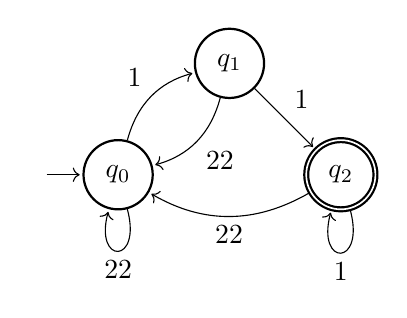
\begin{tikzpicture}[shorten >=1pt,node distance=2cm,on grid,auto]
            \node[state, initial] (q0) {$q_0$};
            \node[state] (q1) [above right=of q0] {$q_1$};
            \node[state, accepting] (q2) [below right=of q1] {$q_2$};
            \path[->] 
                (q0) edge [bend left] node {$1$} (q1)
                      edge [loop below] node {$22$} ()
                (q1) edge [bend left] node {$22$} (q0)
                      edge node {$1$} (q2)
                (q2) edge [bend left] node {$22$} (q0)
                      edge [loop below] node {$1$} ();
        \end{tikzpicture}
    \end{center}
    
    \item[$(ii)$] To recognise the empty language, we can just not include any accepting states in the DFA:
    \begin{center}
        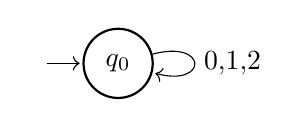
\begin{tikzpicture}[shorten >=1pt,node distance=2cm,on grid,auto]
            \node[state, initial] (q0) {$q_0$};
            \path[->] (q0) edge [loop right] node {$0,1,2$} ();
        \end{tikzpicture}
    \end{center}

    \item[$(iii)$] To accept $\varepsilon$, we make the initial state accepting, and to reject every other word, we immediately move to a dead state upon reading any other symbol:
    \begin{center}
        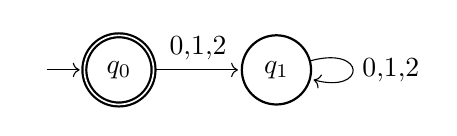
\begin{tikzpicture}[shorten >=1pt,node distance=2cm,on grid,auto]
            \node[state, initial, accepting] (q0) {$q_0$};
            \node[state] (q1) [right=of q0] {$q_1$};
            \path[->]
                (q0) edge node {$0,1,2$} (q1)
                (q1) edge [loop right] node {$0,1,2$} ();
        \end{tikzpicture}
    \end{center}

    \item[$(iv)$] We need two states to keep track of which of the two symbols was last read:
    \begin{center}
        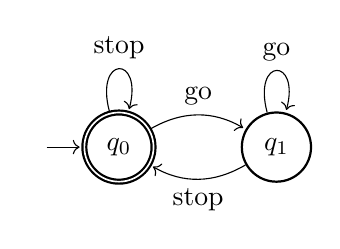
\begin{tikzpicture}[shorten >=1pt,node distance=2cm,on grid,auto]
            \node[state, initial, accepting] (q0) {$q_0$};
            \node[state] (q1) [right=of q0] {$q_1$};
            \path[->]
                (q0) edge [bend left] node {go} (q1)
                      edge [loop above] node {stop} ()
                (q1) edge [bend left] node {stop} (q0)
                      edge [loop above] node {go} ();
        \end{tikzpicture}
    \end{center}

    \item[$(v)$] We can immediately check for the prefix and go into an looping accepting state if it is matched, or otherwise match on the suffix at each exit point:
    \begin{center}
        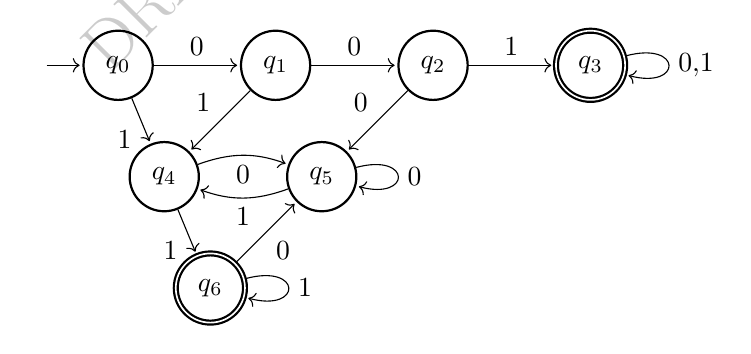
\begin{tikzpicture}[shorten >=1pt,node distance=2cm,on grid,auto]
            \node[state, initial] (q0) {$q_0$};
            \node[state] (q1) [right=of q0] {$q_1$};
            \node[state] (q2) [right=of q1] {$q_2$};
            \node[state, accepting] (q3) [right=of q2] {$q_3$};
            \node[state] (q4) [below left=of q1] {$q_4$};
            \node[state] (q5) [right=of q4] {$q_5$};
            \node[state, accepting] (q6) [below left=of q5] {$q_6$};
            \path[->]
                (q0) edge node {$0$} (q1)
                     edge [swap] node {$1$} (q4)
                (q1) edge node {$0$} (q2)
                     edge [swap] node {$1$} (q4)
                (q2) edge node {$1$} (q3)
                     edge [swap] node {$0$} (q5)
                (q3) edge [loop right] node {$0,1$} ()
                (q4) edge [in=160,out=20,swap] node {$0$} (q5)
                     edge [swap] node {$1$} (q6)
                (q5) edge [in=340,out=200] node {$1$} (q4)
                     edge [loop right] node {$0$} ()
                (q6) edge [loop right] node {$1$} ()
                     edge [swap] node {$0$} (q5);
        \end{tikzpicture}
    \end{center}
\end{enumerate}



\begin{questionbox}{$Q3$}
    Consider the following automata:
    \begin{center}
        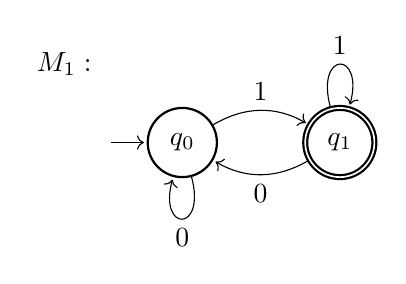
\begin{tikzpicture}[shorten >=1pt,node distance=2cm,on grid,auto]
            \node at (-1.5,1) {$M_1:$};
            \node[state, initial] (q0) {$q_0$};
            \node[state, accepting] (q1) [right=of q0] {$q_1$};
            \path[->]
                (q0) edge [bend left] node {$1$} (q1)
                     edge [loop below] node {$0$} ()
                (q1) edge [bend left] node {$0$} (q0)
                     edge [loop above] node {$1$} ();
        \end{tikzpicture}
        \qquad
        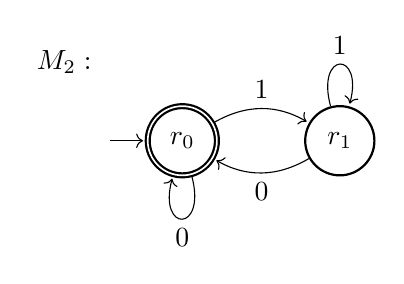
\begin{tikzpicture}[shorten >=1pt,node distance=2cm,on grid,auto]
            \node at (-1.5,1) {$M_2:$};
            \node[state, initial, accepting] (r0) {$r_0$};
            \node[state,] (r1) [right=of r0] {$r_1$};
            \path[->]
                (r0) edge [bend left] node {$1$} (r1)
                     edge [loop below] node {$0$} ()
                (r1) edge [bend left] node {$0$} (r0)
                     edge [loop above] node {$1$} ();
        \end{tikzpicture}
    \end{center}
    \begin{enumerate}
        \item[$(i)$] Construct an automaton accepting $L(M_1)\cap L(M_2)$.
        
        \item[$(ii)$] Prove that regular languages are closed under intersection.
    
        \item[$(iii)$] Construct an automaton for the language $\{0,1\}^\ast\setminus\bigl(L(M_1)\cap L(M_2)\bigr)$.
    
        \item[$(iv)$] Prove that regular languages are closed under complementation.
    \end{enumerate}
\end{questionbox}

\bigskip

\begin{enumerate}
    \item[$(i)$] By pairing up the states, we have:
    \begin{center}
        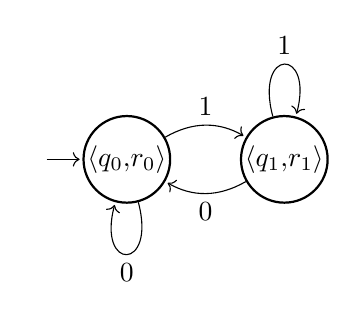
\begin{tikzpicture}[shorten >=1pt,node distance=2cm,on grid,auto,state/.append style={minimum size=11mm,inner sep=0pt}]
            \node[state, initial] (q0) {$\langle q_0,r_0\rangle$};
            \node[state] (q1) [right=of q0] {$\langle q_1,r_1\rangle$};
            \path[->]
                (q0) edge [bend left] node {$1$} (q1)
                     edge [loop below] node {$0$} ()
                (q1) edge [bend left] node {$0$} (q0)
                     edge [loop above] node {$1$} ();
        \end{tikzpicture}
    \end{center}
    (the other state pairs are not reachable from $\langle q_0,r_0\rangle$.)

    Alternatively, we could notice that the two languages are disjoint, and just give the DFA for the empty language:
    \begin{center}
        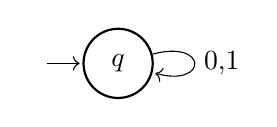
\begin{tikzpicture}[shorten >=1pt,node distance=2cm,on grid,auto]
            \node[state, initial] (q) {$q$};
            \path[->] (q) edge [loop right] node {$0,1$} ();
        \end{tikzpicture}
    \end{center}
    
    \item[$(ii)$] The idea is to run both automata at the same time by operating on pairs of states, where a transition $(q,r)\xrightarrow{a}(q',r')$ exists if and only if both $q\xrightarrow{a}q'$ and $r\xrightarrow{a}r'$ exist in the two original automata.
    
    Let $L_1$ and $L_2$ be regular, with $L_i=L(M_i)$ for DFA $M_i=(Q_i,\Sigma,\delta_i,q_0^i,F_i)$. Construct the automata $M=(Q,\Sigma,\delta,q_0,F)$ by:
    \begin{align*}
        Q&\coloneqq Q_1\times Q_2\\
        \delta&\coloneqq\delta_1\times\delta_2\\
        \delta\bigl(\langle q_1,q_2\rangle,a\bigr)&=\langle\delta_1(q_1,a),\delta_2(q_2,a)\rangle\\
        q_0&\coloneqq\langle q_0^1,q_0^2\rangle\\
        F&\coloneqq F_1\times F_2
    \end{align*}
    Then, $L(M)=L(M_1)\cap L(M_2)$. This is because, any accepting run of $M$ on $w=a_0\cdots a_n$ consists of accepting run of $M_1$ in the first component, and an accepting run of $M_2$ in the second:
    \begin{center}
        \begin{tblr}{colspec={lccccccccccc}, colsep=2pt}
            $M:$ & $\langle q_0^1,q_0^2\rangle$ & $\xrightarrow{a_0}$ & $\langle q_1^1,q_1^2\rangle$ & $\xrightarrow{a_1}$ & $\langle q_1^1,q_1^2\rangle$ & $\rightarrow$ & $ \cdots$ & $\rightarrow$ & $\langle q_n^1,q_n^2\rangle$ & $\xrightarrow{a_n}$ & $\langle q_{n+1}^1,q_{n+1}^2\rangle$\\[2ex]
            \SetCell[c=12]{c}\rotatebox{90}{$\leftrightsquigarrow$}\\[1.5ex]
            $M_1:$ & $q_0^1$ & $\xrightarrow{a_0}$ & $q_1^1$ & $\xrightarrow{a_1}$ & $q_1^1$ & $\rightarrow$ & $ \cdots$ & $\rightarrow$ & $q_n^1$ & $\xrightarrow{a_n}$ & $q_{n+1}^1$\\
            \SetCell[c=12]{c}and\\
            $M_2:$ & $q_0^2$ & $\xrightarrow{a_0}$ & $q_1^2$ & $\xrightarrow{a_1}$ & $q_1^2$ & $\rightarrow$ & $ \cdots$ & $\rightarrow$ & $q_n^2$ & $\xrightarrow{a_n}$ & $q_{n+1}^2$\\
        \end{tblr}
    \end{center}
    % \begin{gather*}
    %     \langle q_0^1,q_0^2\rangle\xrightarrow{a_0}\langle q_1^1,q_1^2\rangle\xrightarrow{a_1}\langle q_1^1,q_1^2\rangle\rightarrow\cdots\rightarrow\langle q_{n-1}^1,q_{n-1}^2\rangle\xrightarrow{a_{n-1}}\langle q_n^1,q_n^2\rangle\xrightarrow{a_n}\langle q_{n+1}^1,q_{n+1}^2\rangle
    % \end{gather*}
    
    Formally by induction:

    \begin{claim}
        For all words $s\in\Sigma^\ast$,
        \begin{equation*}
            \hat\delta\bigl(q_0,s\bigr)=\bigl\langle\hat\delta_1(q_0^1,s),\hat\delta_2(q_0^2,s)\bigr\rangle
        \end{equation*}
    \end{claim}
    \begin{proof}
        By induction on $|s|$. If $|s|=0$, then $s=\varepsilon$, so:
        \begin{equation*}
            \hat\delta(q,\varepsilon)=q=\langle q_0^1,q_0^2\rangle=\bigl\langle\hat\delta_1(q_0^1,\varepsilon),\hat\delta_2(q_0^2,\varepsilon)\bigr\rangle
        \end{equation*}
    
        Otherwise, suppose $s=wa$ with $w\in\Sigma^\ast$ and $a\in\Sigma$:
        \begin{align*}
            \hat\delta\bigl(\langle q_0^1,q_0^2\rangle,wa\bigr)&=\delta\bigl(\hat\delta(\langle q_0^1,q_0^2\rangle,w),\,a\bigr)\\
            \intertext{By the induction hypothesis, the run of $M$ on words shorter than $wa$ agrees with the runs of $M_1$ and $M_2$. In particular, $w$ is shorter than $wa$, so $\hat\delta(\langle q_0^1,q_0^2\rangle,w)=\bigl\langle\hat\delta_1(q_0^1,w),\hat\delta_2(q_0^2,w)\bigr\rangle$, which gives:}
            &=\delta\Bigl(\bigl\langle\hat\delta_1(q_0^1,w),\hat\delta_2(q_0^2,w)\bigr\rangle,\,a\Bigr)\\
            &=\bigl\langle\hat\delta_1(q_0^1,wa),\hat\delta_1(q_0^2,wa)\bigr\rangle\qedhere
        \end{align*}
    \end{proof}
    Now, $M$ accepts a string $s$ if and only if $\hat\delta\bigl(\langle q_0^1,q_0^2\rangle,s\bigr)\in F$ (that is, its run on $s$ is accepting). By the above, this is equivalent to $\bigl\langle\hat\delta_1(q_0^1,s),\hat\delta_1(q_0^2,s)\bigr\rangle\in F_1\times F_2$, which holds if and only if both components hold. That is, $\hat\delta_1(q_0^1,s)\in F_1$ ($M_1$ accepts $s$) and $\hat\delta_2(q_0^2,s)\in F_2$ ($M_2$ accepts $s$). So $M$ accepts $s$ if and only if $M_1$ and $M_2$ accept $s$.



    \item[$(iii)$] To take the complement of the language, we can invert the accepting and rejecting states of the previous automaton:
    \begin{equation*}
        \overline{M}=(Q,\,\Sigma,\,\delta,\,q_0,\,Q\setminus F)
    \end{equation*}
    
    \item[$(iv)$] This trick works in general: if $M=(Q,\Sigma,\delta,q_0,Q)$ accepts $L$, then 
    \begin{equation*}
        \overline{M}=(Q,\Sigma,\delta,q_0,Q\setminus F)
    \end{equation*}
    accepts $\Sigma^\ast\setminus L$.
\end{enumerate}







\begin{questionbox}{$Q4$}
    Construct finite automata that recognise the following languages over $\Sigma=\{0,1\}$:
    \begin{enumerate}
        \item[$(i)$] $L_1=\{w\mid w=0^{2n}\text{ or }w=1^{3n}\text{ or }w=u101v\text{ for some }u,v\in\Sigma^\ast\}$
        
        \item[$(ii)$] $L_2=\{w\mid w\text{ has prefix 001 and suffix 00}\}\cup\{\varepsilon\}$
    \end{enumerate}
    Hint: you may want to construct NFA rather than DFA.
\end{questionbox}

\bigskip

\begin{enumerate}
    \item[$(i)$] This is the union of three languages, so we can just construct the three automata separately, then connect to their starting states with $\varepsilon$-transitions:
    \begin{center}
        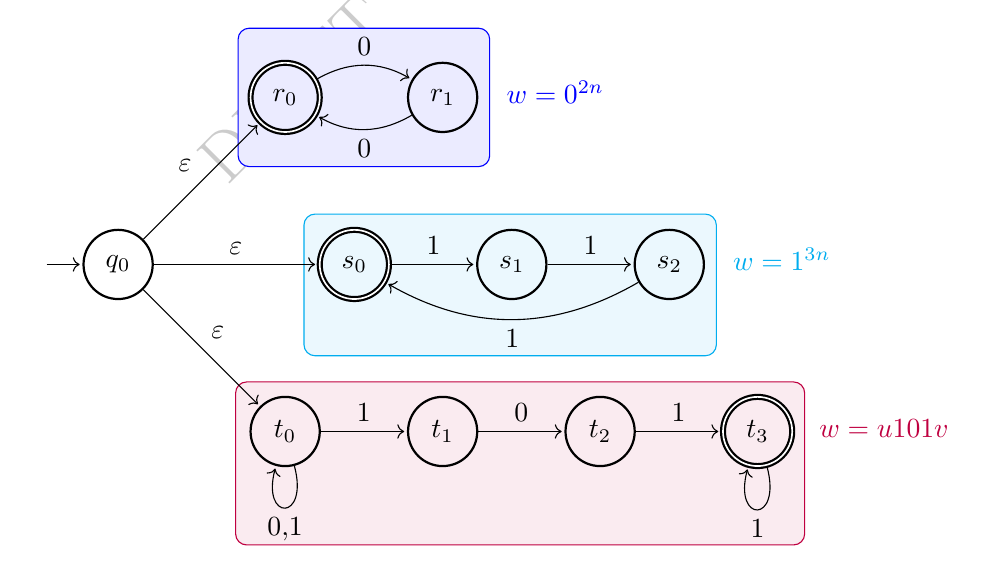
\begin{tikzpicture}[shorten >=1pt,node distance=2cm,on grid,auto]
            \node[state, initial] (q0) {$q_0$};
            \node[state, accepting] (r0) [above right=3cm of q0] {$r_0$};
            \node[state] (r1) [right=of r0] {$r_1$};
            \node[state, accepting] (s0) [right=3cm of q0] {$s_0$};
            \node[state] (s1) [right=of s0] {$s_1$};
            \node[state] (s2) [right=of s1] {$s_2$};
            \node[state] (t0) [below right=3cm of q0] {$t_0$};
            \node[state] (t1) [right=of t0] {$t_1$};
            \node[state] (t2) [right=of t1] {$t_2$};
            \node[state, accepting] (t3) [right=of t2] {$t_3$};
            \path[->]
                (q0) edge node {$\varepsilon$} (r0)
                     edge node {$\varepsilon$} (s0)
                     edge node {$\varepsilon$} (t0)
                (r0) edge [bend left] node {$0$} (r1)
                (r1) edge [bend left] node {$0$} (r0)
                (s0) edge node {$1$} (s1)
                (s1) edge node {$1$} (s2)
                (s2) edge [bend left] node {$1$} (s0)
                (t0) edge node {$1$} (t1)
                     edge [loop below] node {$0,1$} ()
                (t1) edge node {$0$} (t2)
                (t2) edge node {$1$} (t3)
                (t3) edge [loop below] node {$1$} ();

            \node (r) [right=1.5cm of r1,xshift=-2pt,yshift=2pt] {$\textcolor{blue}{w=0^{2n}}$};
            \node (s) [right=1.5cm of s2,xshift=-2pt,yshift=2pt] {$\textcolor{cyan}{w=1^{3n}}$};
            \node (t) [right=1.5cm of t3,xshift=3pt,yshift=1pt] {$\textcolor{purple}{w=u101v}$};
            
            \coordinate (space) at ($(r0)+(-12pt,-20pt)$) {};
            \coordinate (space2) at ($(r1)+(12pt,20pt)$) {};
            \coordinate (space3) at ($(s2)+(12pt,-28pt)$) {};
            \coordinate (space4) at ($(t3)+(12pt,-36pt)$) {};
            \begin{pgfonlayer}{background}
                \node (box) [draw=blue, fill=blue!8, fit=(space) (space2), inner sep=5pt, rounded corners] {};
                \node (box2) [draw=cyan, fill=cyan!8, fit=(s0) (space3), inner sep=5pt, rounded corners] {};
                \node (box3) [draw=purple, fill=purple!8, fit=(t0) (space4), inner sep=5pt, rounded corners] {};
            \end{pgfonlayer}
        \end{tikzpicture}
    \end{center}
    
    \item[$(ii)$] We can immediately check for the prefix, have a looping state, then check for the suffix using non-determinism:
    \begin{center}
        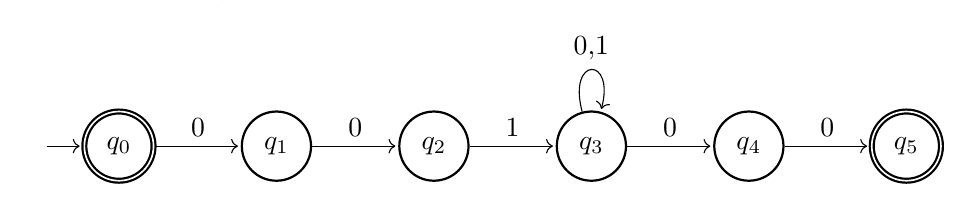
\begin{tikzpicture}[shorten >=1pt,node distance=2cm,on grid,auto]
            \node[state, initial, accepting] (q0) {$q_0$};
            \node[state] (q1) [right=of q0] {$q_1$};
            \node[state] (q2) [right=of q1] {$q_2$};
            \node[state] (q3) [right=of q2] {$q_3$};
            \node[state] (q4) [right=of q3] {$q_4$};
            \node[state, accepting] (q5) [right=of q4] {$q_5$};
            \path[->]
                (q0) edge node {$0$} (q1)
                (q1) edge node {$0$} (q2)
                (q2) edge node {$1$} (q3)
                (q3) edge node {$0$} (q4)
                     edge [loop above] node {$0,1$} ()
                (q4) edge node {$0$} (q5);
        \end{tikzpicture}
    \end{center}
\end{enumerate}










\begin{questionbox}{$Q5$}
    For a word $w\in\Sigma^\ast$, its \textit{reverse} $(w)^r$ is defined recursively by:
    \begin{align*}
        (\varepsilon)^r&\coloneqq\varepsilon\\
        (wa)^r&\coloneqq a(w)^r
    \end{align*}
    \begin{enumerate}
        \item[$(i)$] Let $\Sigma=\{a,b,c\}$. Prove that $(abc)^r=cba$ by unfolding the definition.
        
        \item[$(ii)$] For a language $L$, we define the \textit{reverse language} $L^r$ by
        \begin{equation*}
            L^r\coloneqq\bigl\{(w)^r\mid w\in L\bigr\}
        \end{equation*}
        Prove that $L^r$ is regular if $L$ is regular.
    \end{enumerate}
\end{questionbox}

\bigskip



\begin{enumerate}
    \item[$(i)$] $(abc)^r=c(ab)^r=cb(a)^r=cba(\varepsilon)^r=cba\varepsilon=cba$.
    
    \item[$(ii)$] Let $L=L(M)$ for a DFA $M=(Q,\Sigma,\delta,q_0,F)$.
    
    Intuitively, reversing all of the arrows in the state diagram for $M$ and swapping the initial and accepting states should yield a state diagram that accepts the reverse of every word in $L$. However, $M$ may have multiple accept states, so this naïve inversion doesn't yield a valid DFA (or NFA). However, we may amend this by adjoining a new initial state $q_I$ with $\varepsilon$-transitions to the intended initial states.

    Construct the NFA $M^r=\bigl(Q\cup\{q_I\},\Sigma,\delta^r,q_I,\{q_0\}\bigr)$ by
    \begin{align*}
        \delta^r(q_I,\varepsilon)&\coloneqq F\\
        \delta^r(q_I,a)&\coloneqq\varnothing\text{ for all }a\in\Sigma\\
        \delta^r(q,\varepsilon)&\coloneqq F\text{ for all }q\in Q\text{ (since we started with a DFA)}\\
        \delta^r(q,a)&\coloneqq\bigl\{q'\in Q\mid\delta(q',a)=q\bigr\}
    \end{align*}
\end{enumerate}

\begin{example}
    Consider the language $L\subseteq\{0,1\}^\ast$ defined by $L=\{\text{every $1$ is followed by $00$}\}$, accepted by the DFA
    \begin{center}
        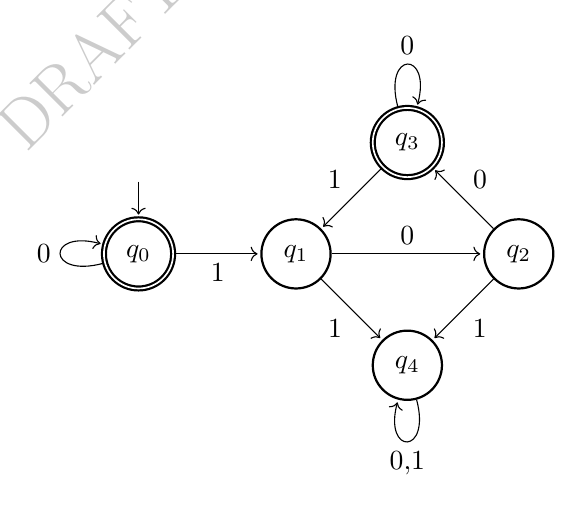
\begin{tikzpicture}[shorten >=1pt,node distance=2cm,on grid,auto]
            \node[state, initial above, accepting] (q_0) {$q_0$};
            \node[state] (q_1) [right=of q_0] {$q_1$};
            \node[state, accepting] (q_3) [above right=of q_1] {$q_3$};
            \node[state] (q_2) [below right=of q_3] {$q_2$};
            \node[state] (q_4) [below right=of q_1] {$q_4$};
            \path[->] 
            (q_0) edge [swap]       node {$1$} (q_1)
                  edge [loop left]  node {$0$} ()
            (q_1) edge              node {$0$} (q_2)
                  edge [swap]       node {$1$} (q_4)
            (q_2) edge              node {$1$} (q_4)
                  edge [swap]       node {$0$} (q_3)
            (q_3) edge [swap]       node {$1$} (q_1)
                  edge [loop above] node {$0$} ()
            (q_4) edge [loop below] node {$0,1$} ();
        \end{tikzpicture}
    \end{center}
    By reversing the arrows and adding a new state equipped with $\varepsilon$-transitions to the two previous accepting states, we obtain a state diagram of an NFA that accepts $L^r=\{\text{every $1$ is preceded by $00$}\}$:
    \begin{center}
        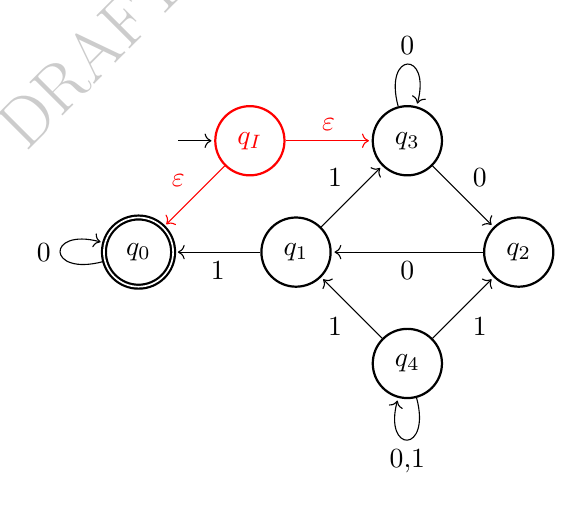
\begin{tikzpicture}[shorten >=1pt,node distance=2cm,on grid,auto]
            \node[state, accepting] (q_0) {$q_0$};
            \node[state, initial, red] (q_I) [above right=of q_0]{$q_I$};
            \node[state] (q_1) [right=of q_0] {$q_1$};
            \node[state] (q_3) [above right=of q_1] {$q_3$};
            \node[state] (q_2) [below right=of q_3] {$q_2$};
            \node[state] (q_4) [below right=of q_1] {$q_4$};
            \path[->] 
            (q_I) edge [swap, red]  node {$\varepsilon$} (q_0)
                  edge [red]        node {$\varepsilon$} (q_3)
            (q_0) edge [loop left]  node {$0$} ()
            (q_1) edge              node {$1$} (q_0)
                  edge              node {$1$} (q_3)
            (q_2) edge              node {$0$} (q_1)
            (q_3) edge              node {$0$} (q_2)
                  edge [loop above] node {$0$} ()
            (q_4) edge              node {$1$} (q_1)
                  edge [swap]       node {$1$} (q_2)
                  edge [loop below] node {$0,1$} ();
        \end{tikzpicture}
    \end{center}
\end{example}





\newpage
\section{Sheet 2}

\begin{questionbox}{$Q1$}
    Construct a DFA equivalent to each of the NFA below, where $\Sigma=\{a,b\}$.
    \begin{enumerate}
        \item[$(i)$]\hspace*{1cm}
        \begin{center}
        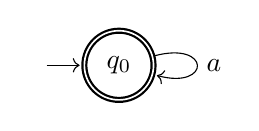
\begin{tikzpicture}[shorten >=1pt,node distance=2cm,on grid,auto]
            \node[state, initial, accepting] (q0) {$q_0$};
            \path[->] (q0) edge [loop right] node {$a$} ();
        \end{tikzpicture}
        \end{center}
        
        \item[$(ii)$]\hspace*{1cm}
        \begin{center}
        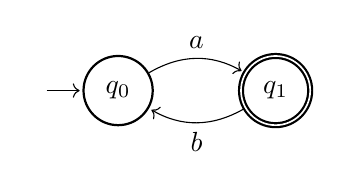
\begin{tikzpicture}[shorten >=1pt,node distance=2cm,on grid,auto]
            \node[state, initial] (q0) {$q_0$};
            \node[state, accepting] (q1) [right=of q0] {$q_1$};
            \path[->]
                (q0) edge [bend left] node {$a$} (q1)
                (q1) edge [bend left] node {$b$} (q0);
        \end{tikzpicture}
        \end{center}
        
        \item[$(iii)$]\hspace*{1cm}
        \begin{center}
        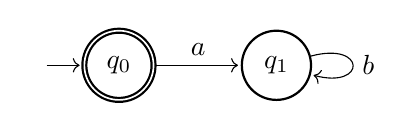
\begin{tikzpicture}[shorten >=1pt,node distance=2cm,on grid,auto]
            \node[state, initial, accepting] (q0) {$q_0$};
            \node[state] (q1) [right=of q0] {$q_1$};
            \path[->]
                (q0) edge node {$a$} (q1)
                (q1) edge [loop right] node {$b$} ();
        \end{tikzpicture}
        \end{center}
        
        \item[$(iv)$]\hspace*{1cm}
        \begin{center}
        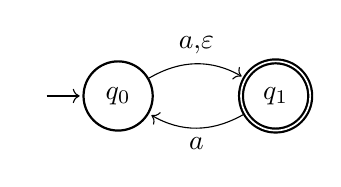
\begin{tikzpicture}[shorten >=1pt,node distance=2cm,on grid,auto]
            \node[state, initial] (q0) {$q_0$};
                \node[state, accepting] (q1) [right=of q0] {$q_1$};
                \path[->]
                (q0) edge [bend left] node {$a,\varepsilon$} (q1)
                (q1) edge [bend left] node {$a$} (q0);
        \end{tikzpicture}
        \end{center}
    
        \item[$(v)$]\hspace*{1cm}
        \begin{center}
        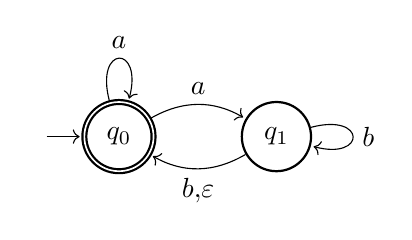
\begin{tikzpicture}[shorten >=1pt,node distance=2cm,on grid,auto]
            \node[state, initial, accepting] (q0) {$q_0$};
            \node[state] (q1) [right=of q0] {$q_1$};
            \path[->]
                (q0) edge [bend left] node {$a$} (q1)
                     edge [loop above] node {$a$} ()
                (q1) edge [bend left] node {$b,\varepsilon$} (q0)
                     edge [loop right] node {$b$} ();
        \end{tikzpicture}
        \end{center}
    
        \item[$(vi)$]\hspace*{1cm}
        \begin{center}
        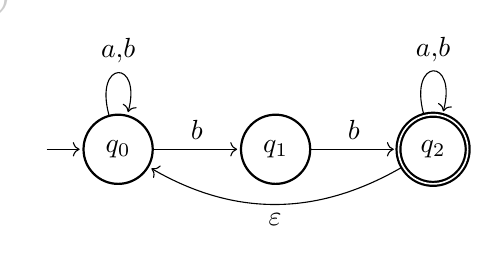
\begin{tikzpicture}[shorten >=1pt,node distance=2cm,on grid,auto]
            \node[state, initial] (q0) {$q_0$};
            \node[state] (q1) [right=of q0] {$q_1$};
            \node[state, accepting] (q2) [right=of q1] {$q_2$};
            \path[->]
                (q0) edge node {$b$} (q1)
                     edge [loop above] node {$a,b$} ()
                (q1) edge node {$b$} (q2)
                (q2) edge [bend left] node {$\varepsilon$} (q0)
                     edge [loop above] node {$a,b$} ();
        \end{tikzpicture}
        \end{center}
    \end{enumerate}
\end{questionbox}

\bigskip

When a DFA is run on a word, we just keep track of a single state; that is, the state $q_i$ that is reached upon reading a prefix of the input string, that can then be overwritten by the state that is reached upon reading the next symbol $s$.

In contrast, when running an NFA, we need to keep track of the set of all states that could be reached after seeing the same prefix, according to the non-deterministic choices made by the automaton. If, however, after a certain prefix has been read, a set $S$ of states can be reached, then the set of symbols reachable upon reading the next symbol $s$ is a deterministic function of $S$ and $s$. That is, while the states reached at each step in an individual run is non-deterministic, the set of states reachable at each step over all possible runs is fully deterministic, and as such, traversing sets of reachable states in this way describes the action of a DFA. This is the strategy of our construction.

Let $N=(Q,\Sigma,\delta,q_0,F)$ be the NFA to be determinised. Then, the DFA $M=(Q',\Sigma,\delta',q_0',F')$ defined by
\begin{itemize}
    \item $Q'=\pazocal{P}(Q)$;
    \item $q_0'=\eclose(q_0)$;
    \item $F'=\{X\subseteq Q:X\cap F\neq\emptyset\}$;
    \item
    $\begin{aligned}[t]
        \delta'(X,a)&=\bigcup_{x\in X}\eclose\bigl(\delta(x,a)\bigr)\\
        &=\Bigl\{z:\exists x\in X: z\in\eclose\bigl(\delta(x,a)\bigr)\Bigr\}
    \end{aligned}$
\end{itemize}
accepts the same language.

\begin{proposition}
    For all $s\in\Sigma^\ast$, $\hat{\delta}(q_0,s)=\hat{\delta}'(q_0',s)$.
\end{proposition}
\begin{proof}
    By induction on $|s|$. If $|s|=0$, then $\hat{\delta}(q_0,s)=\hat{\delta}(q_0,\varepsilon)=\eclose(q_0)=q_0'=\delta'(q_0',\varepsilon)=\hat{\delta}'(q_0',s)$. Otherwise, suppose $s=wa$ with $w\in\Sigma^\ast$, $a\in\Sigma$. Then,
    \begin{align*}
        \hat{\delta}(q_0,s)&=\bigcup_{p\in\hat{\delta}(q_0,w)}\eclose\bigl(\delta(p,a)\bigr)\\
        &=\bigcup_{p\in\hat{\delta}'(q_0',w)}\eclose\bigl(\delta(p,a)\bigr)\\
        &=\delta'\bigl(\hat{\delta}(q_0',w),a\bigr)\\
        &=\hat{\delta}(q_0',s)\qedhere
    \end{align*}
\end{proof}


In this question, there is only one accepting state for each NFA, so we may omit adjoining a new initial state and simply use the accepting state directly.

\begin{enumerate}
    \item[$(i)$]\hspace*{1cm}
    \begin{center}
    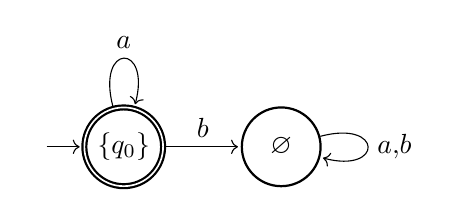
\begin{tikzpicture}[shorten >=1pt,node distance=2cm,on grid,auto,state/.append style={minimum size=10mm,inner sep=0pt}]
        \node[state, initial, accepting] (q0) {$\{q_0\}$};
        \node[state] (em) [right=of q0] {$\varnothing$};
        \path[->]
            (q0) edge node {$b$} (em)
                 edge [loop above] node {$a$} ()
            (em) edge [loop right] node {$a,b$} ();
    \end{tikzpicture}
    \end{center}
    
    \item[$(ii)$]\hspace*{1cm}
    \begin{center}
    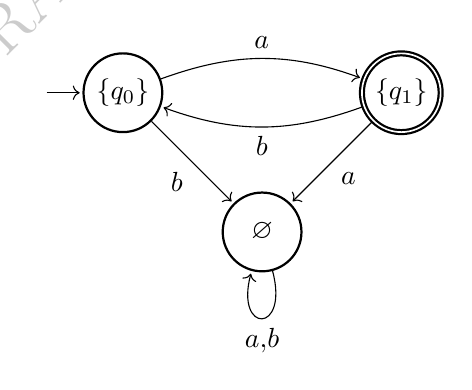
\begin{tikzpicture}[shorten >=1pt,node distance=2cm,on grid,auto,state/.append style={minimum size=10mm,inner sep=0pt}]
        \node[state, initial] (q0) {$\{q_0\}$};
        \node[state] (em) [below right=2.5cm of q0] {$\varnothing$};
        \node[state, accepting] (q1) [above right=2.5cm of em] {$\{q_1\}$};
        \path[->]
            (q0) edge [swap] node {$b$} (em)
                 edge [in=160,out=20] node {$a$} (q1)
            (q1) edge node {$a$} (em)
                 edge [in=340,out=200] node {$b$} (q0)
            (em) edge [loop below] node {$a,b$} ();
    \end{tikzpicture}
    \end{center}

    \item[$(iii)$]\hspace*{1cm}
    \begin{center}
    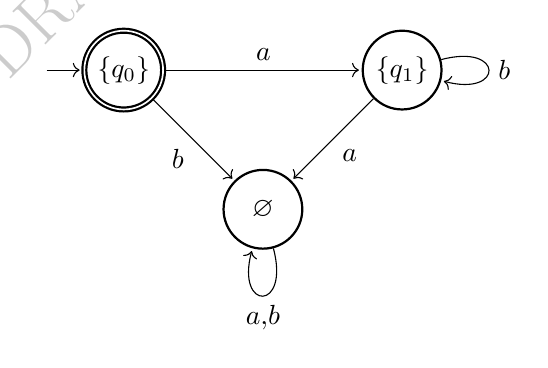
\begin{tikzpicture}[shorten >=1pt,node distance=2cm,on grid,auto,state/.append style={minimum size=10mm,inner sep=0pt}]
        \node[state, initial, accepting] (q0) {$\{q_0\}$};
        \node[state] (em) [below right=2.5cm of q0] {$\varnothing$};
        \node[state] (q1) [above right=2.5cm of em] {$\{q_1\}$};
        \path[->]
            (q0) edge [swap] node {$b$} (em)
                 edge node {$a$} (q1)
            (q1) edge node {$a$} (em)
                 edge [loop right] node {$b$} ()
            (em) edge [loop below] node {$a,b$} ();
    \end{tikzpicture}
    \end{center}

    \item[$(iv)$]\hspace*{1cm}
    \begin{center}
    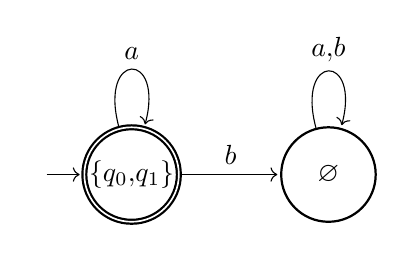
\begin{tikzpicture}[shorten >=1pt,node distance=2cm,on grid,auto,state/.append style={minimum size=12mm,inner sep=0pt}]
        \node[state, initial, accepting] (q01) {$\{q_0,q_1\}$};
        \node[state] (em) [right=2.5cm of q01] {$\varnothing$};
        \path[->]
            (q01) edge node {$b$} (em)
            (q01) edge [loop above] node {$a$} ()
            (em) edge [loop above] node {$a,b$} ();
    \end{tikzpicture}
    \end{center}

    \item[$(v)$]\hspace*{1cm}
    \begin{center}
    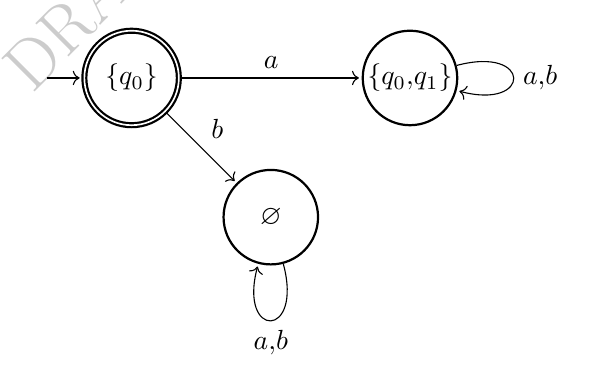
\begin{tikzpicture}[shorten >=1pt,node distance=2cm,on grid,auto,state/.append style={minimum size=12mm,inner sep=0pt}]
        \node[state, initial, accepting] (q0) {$\{q_0\}$};
        \node[state] (em) [below right=2.5cm of q0] {$\varnothing$};
        \node[state] (q01) [above right=2.5cm of em] {$\{q_0,q_1\}$};
        \path[->]
            (q0) edge node {$b$} (em)
                 edge node {$a$} (q01)
            (q01) edge [loop right] node {$a,b$} ()
            (em) edge [loop below] node {$a,b$} ();
    \end{tikzpicture}
    \end{center}

    \item[$(vi)$]\hspace*{1cm}
    \begin{center}
    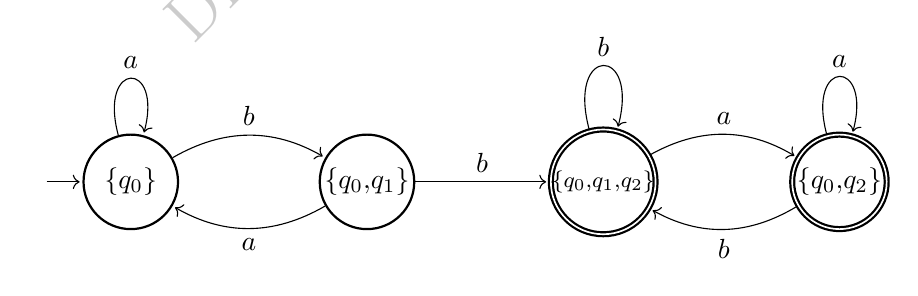
\begin{tikzpicture}[shorten >=1pt,node distance=2cm,on grid,auto,state/.append style={minimum size=12mm,inner sep=0pt}]
        \node[state, initial] (q0) {$\{q_0\}$};
        \node[state] (q01) [right=3cm of q0] {$\{q_0,q_1\}$};
        \node[state, accepting] (q012) [right=3cm of q01] {\footnotesize$\{q_0,q_1,q_2\}$};
        \node[state, accepting] (q02) [right=3cm of q012] {$\{q_0,q_2\}$};

        \path[->]
            (q0)   edge [bend left] node {$b$} (q01)
                   edge [loop above] node {$a$} ()
            (q01)  edge node {$b$} (q012)
                   edge [bend left] node {$a$} (q0)
            (q012) edge [bend left] node {$a$} (q02)
                   edge [loop above] node {$b$} ()
            (q02)  edge [bend left] node {$b$} (q012)
                   edge [loop above] node {$a$} ();
    \end{tikzpicture}
    \end{center}
\end{enumerate}











\begin{questionbox}{$Q2$}
    Consider the language $L=(01\cup001\cup010)^\ast$.
    \begin{enumerate}
        \item[$(i)$] Construct an NFA that recognises L.
        
        \item[$(ii)$] Determinise this NFA.
    \end{enumerate}
\end{questionbox}

\bigskip





If $L$ is recognised by $N$, then $L^\ast$ is recognised by the NFA $M=\bigl(Q_1\cup\{q_0\},\Sigma,\delta,q_1,F_1,\bigr)$ formed by adding a new starting state $q_0$ that is also accepting (in order to accept the empty string) with an $\varepsilon$-transition to the previous start state, then adding $\varepsilon$-transitions from the previous accepting states to the start state (to allow for arbitrary concatenations of words accepted by $N$):

\begin{center}
\begin{tikzpicture}[shorten >=1pt,node distance=2cm,on grid,auto] 

\end{tikzpicture}
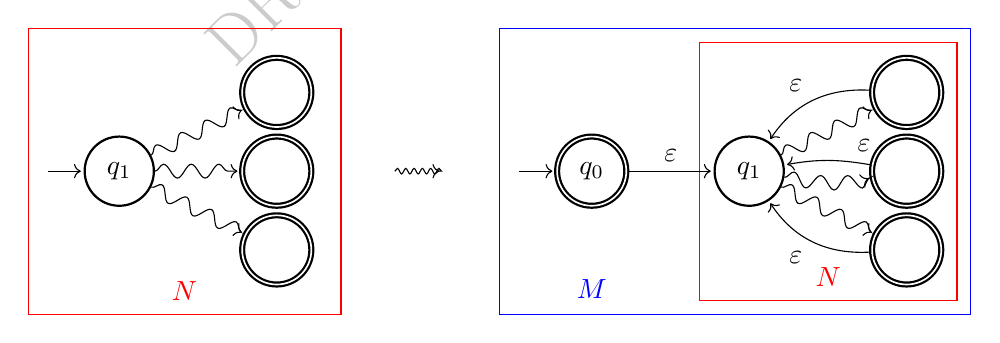
\begin{tikzpicture}[shorten >=1pt,node distance=2cm,on grid,auto]
    \node[state, initial] (q_1) at (-2,0) {$q_1$};
    \node[state, accepting] (q_a) at (0,1) {};
    \node[state, accepting] (q_b) at (0,0) {};
    \node[state, accepting] (q_c) at (0,-1) {};
    \path[->]
    (q_1) edge [decorate, decoration={snake}] (q_a)
          edge [decorate, decoration={snake}] (q_b)
          edge [decorate, decoration={snake}] (q_c);
    \coordinate (space) at ($(q_1.west) + (-10pt,0)$) {};
    \node (box) [draw=red, fit=(space) (q_a) (q_c), inner sep=10pt] {};
    \node [yshift=2ex, red] at (box.south) {$N$};

    \draw[->, decorate, decoration={snake,amplitude=1pt,segment length=3pt}] (1.5,0) -- (2.1,0);

    \node[state, initial, accepting] (q_0) at (4,0) {$q_0$};
    \node[state] (q_11) at (6,0) {$q_1$}; 
    \node[state, accepting] (q_x) at (8,1) {}; 
    \node[state, accepting] (q_y) at (8,0) {}; 
    \node[state, accepting] (q_z) at (8,-1) {}; 
    \path[->]
    (q_11) edge [decorate, decoration={snake}] (q_x)
            edge [decorate, decoration={snake}, bend right=10pt] (q_y)
            edge [decorate, decoration={snake}] (q_z);
    \coordinate (space2) at ($(q_0.west) + (-10pt,0)$) {};
    \node (box2) [draw=red, fit=(q_11) (q_x) (q_z), inner sep=5pt] {};
    \node (box3) [draw=blue, fit=(space2) (q_x) (q_z), inner sep=10pt] {};
    \node [yshift=2ex, red] at (box2.south) {$N$};
    \node [blue] at (4,-1.5) {$M$};
    \path[->]
    (q_0) edge                                      node {$\varepsilon$} (q_11)
    (q_x) edge [bend right, swap]                   node {$\varepsilon$} (q_11)
    (q_y) edge [bend right=10pt, swap, near start]  node {$\varepsilon$} (q_11)
    (q_z) edge [bend left]                          node {$\varepsilon$} (q_11);
\end{tikzpicture}
\end{center}






\bigskip
\begin{enumerate}
    \item[$(i)$]\hspace*{1cm}
    \begin{center}
        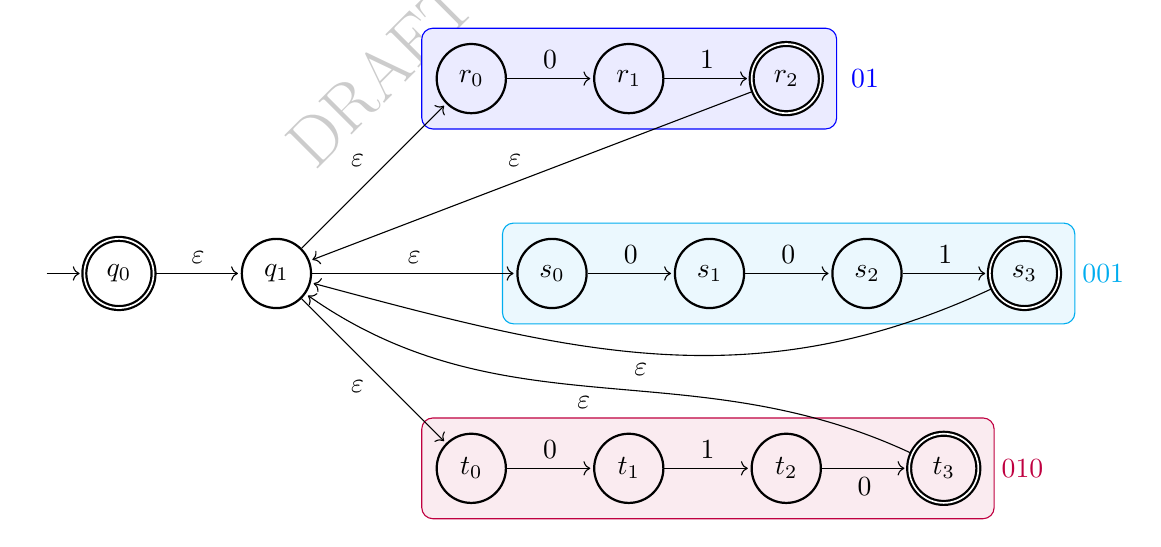
\begin{tikzpicture}[shorten >=1pt,node distance=2cm,on grid,auto]
            \node[state, initial, accepting] (q0) {$q_0$};
            \node[state] (q1) [right=of q0] {$q_1$};
    
            \node[state] (r0) [above right=3.5cm of q1] {$r_0$};
            \node[state] (r1) [right=of r0] {$r_1$};
            \node[state, accepting] (r2) [right=of r1] {$r_2$};
    
            \node[state] (s0) [right=3.5cm of q1] {$s_0$};
            \node[state] (s1) [right=of s0] {$s_1$};
            \node[state] (s2) [right=of s1] {$s_2$};
            \node[state, accepting] (s3) [right=of s2] {$s_3$};
    
            \node[state] (t0) [below right=3.5cm of q1] {$t_0$};
            \node[state] (t1) [right=of t0] {$t_1$};
            \node[state] (t2) [right=of t1] {$t_2$};
            \node[state, accepting] (t3) [right=of t2] {$t_3$};
            
            \path[->]
                (q0) edge node {$\varepsilon$} (q1)
                (q1) edge node {$\varepsilon$} (r0)
                     edge node {$\varepsilon$} (s0)
                     edge [swap] node {$\varepsilon$} (t0)
    
                (r0) edge node {$0$} (r1)
                (r1) edge node {$1$} (r2)
                (r2) edge [swap] node {$\varepsilon$} (q1)
    
                (s0) edge node {$0$} (s1)
                (s1) edge node {$0$} (s2)
                (s2) edge node {$1$} (s3)
                (s3) edge [out=205,in=345] node {$\varepsilon$} (q1)
    
                (t0) edge node {$0$} (t1)
                (t1) edge node {$1$} (t2)
                (t2) edge [swap] node {$0$} (t3)
                (t3) edge [out=155,in=325] node {$\varepsilon$} (q1);
                
            \node (r) [right=1cm of r2] {$\textcolor{blue}{01}$};
            \node (s) [right=1cm of s3] {$\textcolor{cyan}{001}$};
            \node (t) [right=1cm of t3] {$\textcolor{purple}{010}$};
            
            \begin{pgfonlayer}{background}
                \node (box) [draw=blue, fill=blue!8, fit=(r0) (r2), inner sep=5pt, rounded corners] {};
                \node (box2) [draw=cyan, fill=cyan!8, fit=(s0) (s3), inner sep=5pt, rounded corners] {};
                \node (box3) [draw=purple, fill=purple!8, fit=(t0) (t3), inner sep=5pt, rounded corners] {};
            \end{pgfonlayer}
        \end{tikzpicture}
    \end{center}
    We can simplify this to:
    \begin{center}
        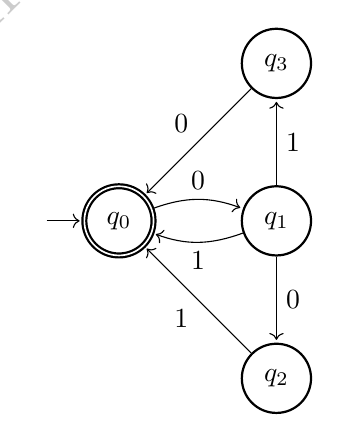
\begin{tikzpicture}[shorten >=1pt,node distance=2cm,on grid,auto]
            \node[state, initial, accepting] (q0) {$q_0$};
            \node[state] (q1) [right=of q0] {$q_1$};
            \node[state] (q2) [below=of q1] {$q_2$};
            \node[state] (q3) [above=of q1] {$q_3$};
    
            
            \path[->]
                (q0) edge [out=20,in=160] node {$0$} (q1)
                (q1) edge [out=200,in=340] node {$1$} (q0)
                     edge node {$0$} (q2)
                     edge [swap] node {$1$} (q3)
                (q2) edge node {$1$} (q0)
                (q3) edge [swap] node {$0$} (q0);
        \end{tikzpicture}
    \end{center}

    \item[$(ii)$] Determinising via subset construction:
    \begin{center}
        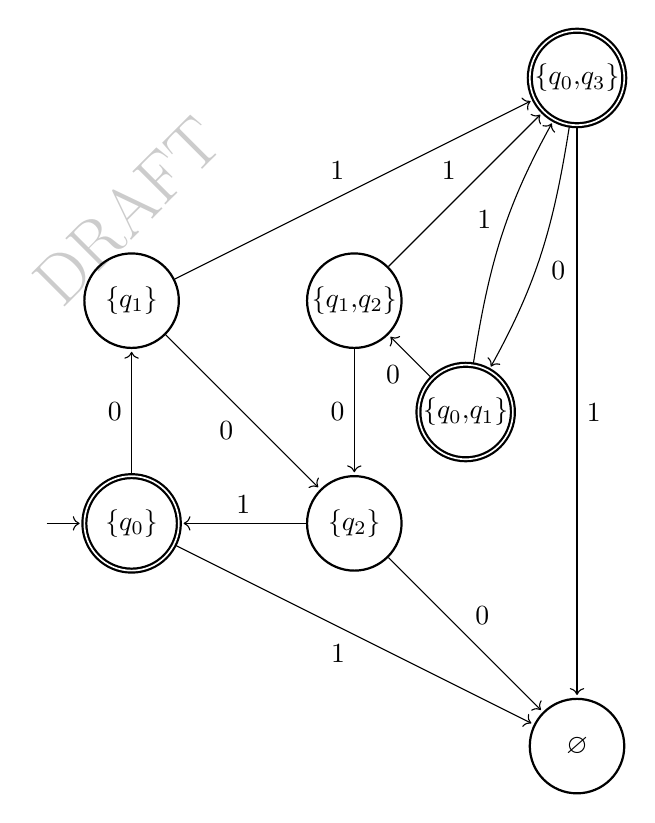
\begin{tikzpicture}[shorten >=1pt,node distance=2cm,on grid,auto,state/.append style={minimum size=12mm,inner sep=0pt}]
            \node[state, initial, accepting] (q0) {$\{q_0\}$};
            \node (space) [above right=of q0]{};
            \node[state] (q1) [above left=of space] {$\{q_1\}$};
            \node[state] (q2) [below right=of space]{$\{q_2\}$};
            \node[state] (q12) [above right=of space] {$\{q_1,q_2\}$};
            \node[state, accepting] (q01) [above right=of q2]{$\{q_0,q_1\}$};
            \node[state, accepting] (q03) [above right=4cm of q12]{$\{q_0,q_3\}$};
            \node[state] (em) [below right=4cm of q2]{$\varnothing$};
            
            \path[->]
                (q0)  edge node {$0$} (q1)
                      edge [swap] node {$1$} (em)
                (q1)  edge [swap] node {$0$} (q2)
                      edge node {$1$} (q03)
                (q2)  edge node {$0$} (em)
                      edge [swap] node {$1$} (q0)
                (q01) edge node {$0$} (q12)
                      edge [out=81,in=241] node {$1$} (q03)
                (q03) edge [in=61,out=261] node {$0$} (q01)
                      edge node {$1$} (em)
                (q12) edge [swap] node {$0$} (q2)
                      edge node {$1$} (q03);
        \end{tikzpicture}
    \end{center}
\end{enumerate}






\begin{questionbox}{$Q3$}
    Prove that the following languages are not regular:
    \begin{enumerate}
        \item[$(i)$] $L_0=\{a^jb^m\mid j>m\geq0\}$;
        
        \item[$(ii)$] $L_1=\{a^ib^jc^k\mid i,j,k\geq0\text{ and if }i=1\text{ then }j=k\}$;
    
        \item[$(iii)$] $L_2=\{0^n1^m0^n\mid m,n\geq0\}$;
    
        \item[$(iv)$] $L_3=\{0^m1^n\mid m\neq n\}$.
    \end{enumerate}
\end{questionbox}

\bigskip




Every regular language is recognised by a DFA -- a deterministic \textit{finite} automaton. Because a DFA only has finitely many states, any sufficiently long string $s$ must repeat a state in the DFA, and hence pass through a cycle:
\begin{center}
    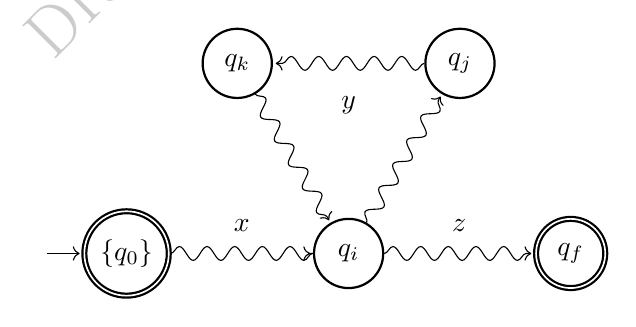
\begin{tikzpicture}[shorten >=1pt,node distance=2cm,on grid,auto]
        \node[state, initial, accepting] (q0) {$\{q_0\}$};
        \node[state] (qi) [right=2.82cm of q0]{$q_i$};
        \node[state] (qj) [above right=of qi,yshift=1cm]{$q_j$};
        \node[state] (qk) [above left=of qi,yshift=1cm]{$q_k$};
        \node[state, accepting] (qf) [right=2.82cm of qi]{$q_f$};
        
        \path[->]
            (q0) edge [decorate, decoration={snake}] node [above,yshift=1ex] {$x$} (qi)
            (qi) edge [decorate, decoration={snake}] (qj)
            (qj) edge [decorate, decoration={snake}] node [below,yshift=-2ex] {$y$} (qk)
            (qk) edge [decorate, decoration={snake}] (qi)
            (qi) edge [decorate, decoration={snake}] node [above,yshift=1ex] {$z$} (qf);
    \end{tikzpicture}
\end{center}
That is, $s$ must be of the form $xyz$, where $x$ is the string read before the cycle, $y$ is the string given by the cycle itself, and $z$ is the trailing string read before accepting.

Because the DFA has no memory, the cycle may be repeated any number of times with the same substring $y$ still be accepted as long as the prefix $x$ and suffix $z$ remain the same. So this diagram accepts any string starting with $x$, followed by any number of $y$s (including zero), followed by $z$.

In fact, this is a complete characterisation of the DFAs that accept an infinite language: because DFAs must have finitely many states, this is the only way an infinite regular language can arise.

\begin{lemma*}[Pumping Lemma for Regular Languages]
    Let $L$ be a regular language. Then, there exists an integer $p\geq 1$ (the \textit{pumping length}), such that for every string $s\in L$ with length $|s|\geq p$, there exists a decomposition $s=x\cdot y\cdot z$ such that
    \begin{itemize}
        \item $|y|\geq1$;
        \item $|xy|\leq p$;
        \item for all $n\geq0$, $x\cdot y^n\cdot z\in L$.
    \end{itemize}
\end{lemma*}

The lemma is just a formalisation of these observations. It says that for every regular language, every word longer than a certain length must be of this form where we can repeat some middle segment of the word and still be accepted.

We can also interpret the pumping length $p$ as the number of internal states of the (minimal) DFA that recognises the language, so if a word is longer than $p$, it must revisit a state, and hence we have a state diagram of the shape above.




\begin{enumerate}
    \item[$(i)$] Suppose $L_0$ is regular and let $p$ be its pumping length. Consider the string $s=a^{p+1}b^p$ of length $2p+1>p$ and let $s=xyz$ be a decomposition with $|y|\geq1$ and $|xy|\leq p$.

    Since $|xy|\leq p$, the substring $xy$ must consist entirely of $a$'s since the first $p+1$ symbols of the string are all $a$'s. By the pumping lemma, $xy^nz\in L$ for all $n\geq0$, but pumping $y$ zero times reduces the number of $a$'s, yielding a string not in $L_0$. So $L_0$ does not satisfy the pumping lemma for regular languages and is hence not a regular language.

    \item[$(ii)$] Recall that regular languages are closed under intersection: by the contrapositive, if $L=U\cap V$ is non-regular and $U$ is regular, then $V$ is non-regular. So, to show that $L_1$ is non-regular, it suffices to show that $L_1\cap U$ is non-regular for some regular language $U$.
    
    Consider the regular language $U$ given by the regular expression $a(b+c)^\ast$. Then,
    \begin{equation*}
        L\coloneqq L_1\cap U=\{ab^jc^j\mid j\geq0\}
    \end{equation*}
    Suppose $L$ is regular and let $p$ be its pumping lenth. Consider the string $s=ab^pc^p$, and let $s=xyz$ be a decomposition with $|y|\geq1$ and $|xy|\leq p$.
    
    Since $|xy|\leq p$, $xy=ab^m$ for some $m<p$. If $x=\varepsilon$, then $y=ab^m$ and pumping $y$ zero times removes the leading $a$. Otherwise, if $x\neq\varepsilon$, then $y=b^n$ for some $n<p$. Now, pumping $y$ changes the number of $b$s but not the number of $c$s. So no such decomposition exists and $L$ is non-regular, and hence $L_1$ is non-regular.

    \item[$(iii)$] Suppose $L_2$ is regular and let $p$ be its pumping length. Consider the string $s=0^p1^{p+1}0^p$ and let $s=xyz$ be a decomposition satisfying the hypotheses of the pumping lemma. Since $|xy|\leq p$, $y$ consists entirely of $0$s, so pumping $y$ changes the number of $0$s in the initial segment, which leaves the language.

    \item[$(iv)$] Regular languages are closed under complementation, so it suffices to show that $\overline{L_3}=\{0^n1^n\}$ is non-regular. Suppose $\overline{L_3}$ is regular and let $p$ be its pumping length. Consider the string $s=0^p1^p$ with a decomposition $s=xyz$ satisfying the hypotheses of the pumping lemma. Since $|xy|\leq p$, $y$ consists entirely of $0$s, so pumping $y$ changes the number of $0$s in the initial segment, which leaves the language.
\end{enumerate}





\begin{questionbox}{$Q4$}
    Consider the following language over the alphabet $\Sigma=\{a,b\}$:
    \begin{equation*}
        L=\left\{w\;\middle|\;\begin{gathered}
            w\text{ has an even number of }a\text{'s,}\\
            \text{an odd number of }b\text{'s,}\\
            \text{and does not contain the substring }ab
        \end{gathered}
        \right\}
    \end{equation*}
    \begin{enumerate}
        \item[$(i)$] Prove that $L$ is regular.
        
        \item[$(ii)$] Find a regular expression that generates $L$.
    \end{enumerate}
\end{questionbox}

\bigskip


First note that $0$ is not an odd number, so $w$ contains at least one $b$; and since $w$ cannot contain the substring $ab$, all of the $a$'s must appear after the $b$(s). So, equivalently, $L$ has the simpler presentation $L=\{b^{2n+1}a^{2n}\}$.

\begin{enumerate}
    \item[$(i)$] To show that $L$ is regular it suffices to provide an NFA recognising $L$:
    \begin{center}
    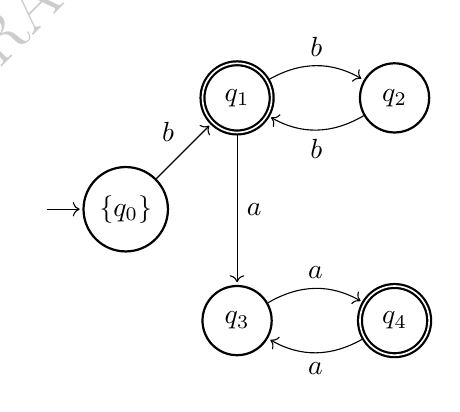
\begin{tikzpicture}[shorten >=1pt,node distance=2cm,on grid,auto]
        \node[state, initial] (q0) {$\{q_0\}$};
        \node[state, accepting] (q1) [above right=of q0]{$q_1$};
        \node[state] (q2) [right=of q1]{$q_2$};
        \node[state] (q3) [below right=of q0]{$q_3$};
        \node[state, accepting] (q4) [right=of q3]{$q_4$};
        
        \path[->]
            (q0) edge node {$b$} (q1)
            (q1) edge [bend left] node {$b$} (q2)
            (q1) edge node {$a$} (q3)
            (q2) edge [bend left] node {$b$} (q1)
            (q3) edge [bend left] node {$a$} (q4)
            (q4) edge [bend left] node {$a$} (q3);
    \end{tikzpicture}
    \end{center}
    
    \item[$(ii)$] Using $L=\{b^{2n+1}a^{2n}\}$, this becomes simple:
    \begin{equation*}
        b(bb)^\ast(aa)^\ast
    \end{equation*}
\end{enumerate}











\begin{questionbox}{$Q4$}
    Consider the following DFA:
    \begin{center}
    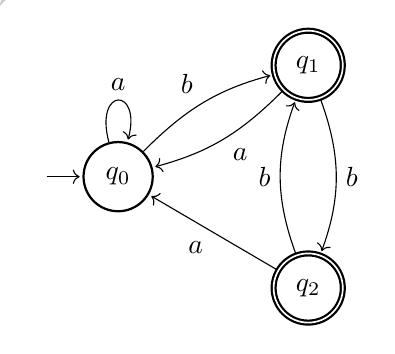
\begin{tikzpicture}[shorten >=1pt,node distance=2cm,on grid,auto]
        \node[state, initial] (q0) {$q_0$};
        \node[state, accepting] (q1) [above right=of q0,xshift=1cm]{$q_1$};
        \node[state, accepting] (q2) [below right=of q0,xshift=1cm]{$q_2$};
        
        \path[->]
            (q0) edge [loop above] node {$a$} ()
                 edge [out=45,in=195] node {$b$} (q1)
            (q1) edge [out=225,in=15] node {$a$} (q0)
                 edge [out=290,in=70] node {$b$} (q2)
            (q2) edge node {$a$} (q0)
                 edge [out=110,in=250] node {$b$} (q1);
    \end{tikzpicture}
    \end{center}

    \begin{enumerate}
        \item[$(i)$] Show that $q_1$ and $q_2$ are bisimilar by giving a bisimulation $R\ni\langle q_1,q_2\rangle$.
        
        \item[$(ii)$] Compute a regular expression equivalent to the automaton.
        
        \item[$(iii)$] Prove the following result:
        \begin{theorem*}
            States that are bisimilar are equivalent.
        \end{theorem*}
    \end{enumerate}
\end{questionbox}

\bigskip



Recall that a bisimulation on a DFA $M=(Q,\Sigma,\delta,q_0,F)$ is a relation $R\subseteq Q\times Q$ on states such that, for any $\langle q,q'\rangle\in R$:
\begin{itemize}
    \item Acceptance agreement: $q\in F$ if and only if $q'\in F$;
    
    \item Step correspondence: for every $a\in\Sigma$, $\bigl\langle\delta(q,a),\delta(q',a)\bigr\rangle\in R$.
\end{itemize}
That is, two states are bisimilar if they agree on $\varepsilon$, and any single step from the two states yields bisimilar states.

While not strictly required by the definition, it is often sensible to add the diagonal elements $\langle q_i,q_i\rangle$ to $R$ (the \textit{reflexive closure}) since the conditions are trivial for such pairs, and similarly, if $\langle q_i,q_j\rangle\in R$, it can be helpful to add the reversed pair $\langle q_j,q_i\rangle$ to $R$ (the \textit{symmetric closure}) since the conditions are symmetric in $q_i$ and $q_j$.


\begin{enumerate}
    \item[$(i)$] We require $\langle q_1,q_2\rangle\in R$. Taking the symmetric reflexive closure, we have:
    \begin{equation*}
        R=\bigl\{\langle q_0,q_0\rangle,\langle q_1,q_1\rangle,\langle q_2,q_2\rangle,\langle q_1,q_2\rangle\langle q_2,q_1\rangle\bigr\}
    \end{equation*}

    The two conditions are trivial for all of the reflexive pairs; and we only need to check one of $\langle q_1,q_2\rangle$ and $\langle q_2,q_1\rangle$.
    
    We verify the two conditions for $\langle q_1,q_2\rangle\in R$:
    \begin{itemize}
        \item Acceptance agreement: $q_1\in F$ and $q_2\in F$;
        
        \item Step correspondence:
        \begin{align*}
            \bigl\langle\delta(q_1,a),\delta(q_2,a)\bigr\rangle&=\langle q_0,q_0\rangle\in R\\
            \bigl\langle\delta(q_1,b),\delta(q_2,b)\bigr\rangle&=\langle q_2,q_1\rangle\in R
        \end{align*}
    \end{itemize}
    so $R$ is a bisimulation.
\end{enumerate}


\bigskip

Recall that a GNFA is a $5$-tuple $(Q,\Sigma,q_\text{start},q_\text{accept},\delta)$, consisting of
\begin{itemize}
    \item a finite set $Q$ of states;
    \item a finite alphabet $\Sigma$;
    \item the start state, $q_\text{start}\in Q$;
    \item the accept state, $q_\text{accept}\in Q$;
    \item and a transition function $\delta:\bigl(Q\setminus\{q_\text{accept}\}\bigr)\times\bigl(Q\setminus\{q_\text{start}\}\bigr)\rightarrow\mathcal{R}$, where $\mathcal{R}$ is the set of all regular expressions over $\Sigma$.
\end{itemize}
Intuitively, a GNFA is an NFA with at most one transition (technically, exactly one, but we may omit the edge in state diagrams when the expression is $\emptyset$) between any two states, but labelled with a regular expression instead of just a single alphabet symbol.

We can convert a DFA into a regular expression as follows:

We first transform the DFA into a GNFA as follows:
\begin{enumerate}
    \item Add a new start state with an $\varepsilon$-transition to the previous start state.
    \item Add a new accepting state with $\varepsilon$-transitions from the previous accepting states to this state.
    \item Any transitions with multiple labels may be replaced with a transition labelled with the union of the previous labels.
\end{enumerate}
This GNFA may then be converted into a regular expression as follows:
\begin{enumerate}
    \item If there are only two states, then we are done, as these must be the unique start and accepting states, and transition connecting them is a regular expression.
    \item Otherwise, select some state $q_r\in Q\setminus\{q_\text{start},q_\text{end}\}$. Then, simultaneously for all $(q_i,q_j)\in\bigl(Q\setminus\{q_\text{start},q_r\}\bigr)\times\bigl(Q\setminus\{q_\text{end},q_r\}\bigr)$, we replace the transitions

    \begin{center}
    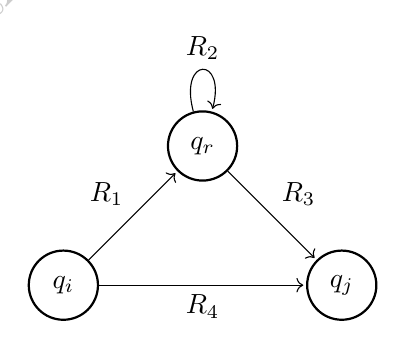
\begin{tikzpicture}[shorten >=1pt,node distance=2.5cm,on grid,auto] 
        \node[state] (q_r) {$q_r$}; 
        \node[state] (q_i) [below left=of q_r] {$q_i$}; 
        \node[state] (q_j) [below right=of q_r] {$q_j$}; 
        \path[->] 
        (q_r) edge              node {$R_3$} (q_j)
              edge [loop above] node {$R_2$} ()
        (q_i) edge              node {$R_1$} (q_r)
              edge [swap]       node {$R_4$} (q_j);
    \end{tikzpicture}
    \end{center}
    by the single edge

    \begin{center}
    \begin{tikzpicture}[shorten >=1pt,node distance=3.5cm,on grid,auto] 
        \node[state] (q_i) {$q_i$}; 
        \node[state] (q_j) [right=of q_i] {$q_j$}; 
        \path[->] 
        (q_r) edge  node {$R_1\cdot R_2^\ast\cdot R_3+R_4$} (q_j);
    \end{tikzpicture}
    \end{center}
    Once this has been done, we may remove $q_r$ from the diagram, then pick a new state to be $q_r$, until the diagram has only the initial and accepting state remaining.
\end{enumerate}


\begin{enumerate}
    \item[$(ii)$] The state deleted at each stage is highlighted in \textcolor{blue}{blue}.
    
    \begin{center}
    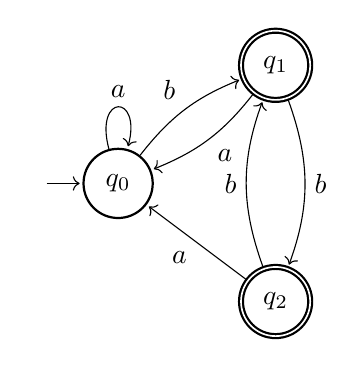
\begin{tikzpicture}[shorten >=1pt,on grid,auto]
        \coordinate (qs) at (0,0);
        \coordinate (qa) at (6,0);
        \node[state, initial] (q0) at (2,0) {$q_0$};
        \node[state, accepting] (q1) at (4,1.5) {$q_1$};
        \node[state, accepting] (q2) at (4,-1.5) {$q_2$};

    \path[->]
        (q0) edge [loop above] node {$a$} ()
             edge [out=52,in=202] node {$b$} (q1)
        (q1) edge [out=232,in=22] node {$a$} (q0)
             edge [out=290,in=70] node {$b$} (q2)
        (q2) edge node {$a$} (q0)
             edge [out=110,in=250] node {$b$} (q1);
    \end{tikzpicture}
    \end{center}
    \vspace*{1cm}
    \begin{center}
    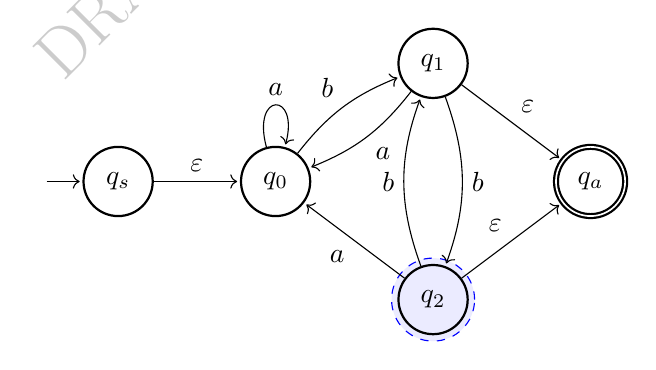
\begin{tikzpicture}[shorten >=1pt,on grid,auto]

        \node[state, initial] (qs) at (0,0) {$q_s$};
        \node[state] (q0) at (2,0) {$q_0$};
        \node[state] (q1) at (4,1.5) {$q_1$};
        \node[state] (q2) at (4,-1.5) {$q_2$};
        \node[state, accepting] (qa) at (6,0) {$q_a$};

        \begin{pgfonlayer}{background}
            \draw[draw=blue,dashed,fill=blue!8] (q2) circle (15pt);
        \end{pgfonlayer}
            
        \path[->]
            (qs) edge node {$\varepsilon$} (q0)
            (q0) edge [loop above] node {$a$} ()
                 edge [out=52,in=202] node {$b$} (q1)
            (q1) edge [out=232,in=22] node {$a$} (q0)
                 edge [out=290,in=70] node {$b$} (q2)
                 edge node {$\varepsilon$} (qa)
            (q2) edge node {$a$} (q0)
                 edge [out=110,in=250] node {$b$} (q1)
                 edge node {$\varepsilon$} (qa);
    \end{tikzpicture}
    \end{center}
    \vspace*{1cm}
    \begin{center}
    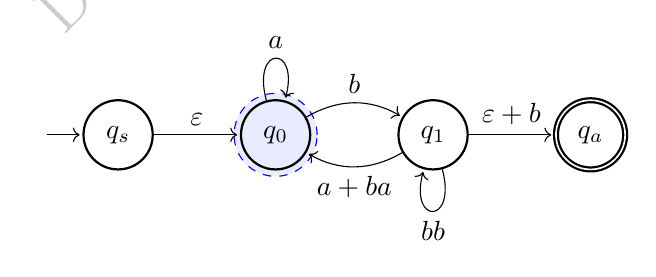
\begin{tikzpicture}[shorten >=1pt,on grid,auto]
        \node[state, initial] (qs) at (0,0) {$q_s$};
        \node[state] (q0) at (2,0) {$q_0$};
        \node[state] (q1) at (4,0) {$q_1$};
        \node[state, accepting] (qa) at (6,0) {$q_a$};

        \begin{pgfonlayer}{background}
            \draw[draw=blue,dashed,fill=blue!8] (q0) circle (15pt);
        \end{pgfonlayer}
            
        \path[->]
            (qs) edge node {$\varepsilon$} (q0)
            (q0) edge [loop above] node {$a$} ()
                 edge [bend left] node {$b$} (q1)
            (q1) edge [bend left] node {$a+ba$} (q0)
                 edge [loop below] node {$bb$} ()
                 edge node {$\varepsilon+b$} (qa);
    \end{tikzpicture}
    \end{center}
    \vspace*{1cm}
    \begin{center}
    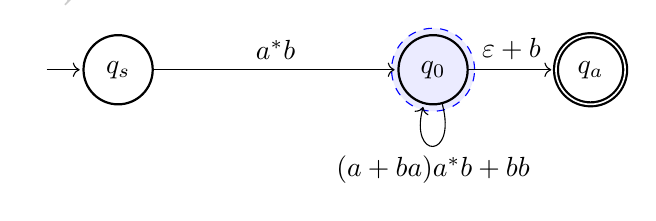
\begin{tikzpicture}[shorten >=1pt,on grid,auto]
        \node[state, initial] (qs) at (0,0) {$q_s$};
        \node[state] (q1) at (4,0) {$q_0$};
        \node[state, accepting] (qa) at (6,0) {$q_a$};

        \begin{pgfonlayer}{background}
            \draw[draw=blue,dashed,fill=blue!8] (q1) circle (15pt);
        \end{pgfonlayer}
            
        \path[->]
            (qs) edge node {$a^\ast b$} (q1)
            (q1) edge [loop below] node {$(a+ba)a^\ast b+bb$} ()
                 edge node {$\varepsilon+b$} (qa);
    \end{tikzpicture}
    \end{center}
    \vspace*{1cm}
    \begin{center}
    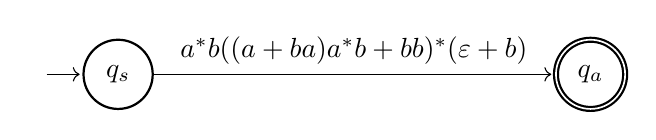
\begin{tikzpicture}[shorten >=1pt,on grid,auto]
        \node[state, initial] (qs) at (0,0) {$q_s$};
        \node[state, accepting] (qa) at (6,0) {$q_a$};

        \path[->]
            (qs) edge node {$a^\ast b((a+ba)a^\ast b+bb)^\ast(\varepsilon+b)$} (qa);
    \end{tikzpicture}
    \end{center}
    So a regular expression equivalent to the original DFA is $a^\ast b((a+ba)a^\ast b+bb)^\ast(\varepsilon+b)$.

    We could have also identified the bisimilar states to obtain a simpler DFA before converting it into a GNFA:
    \begin{center}
    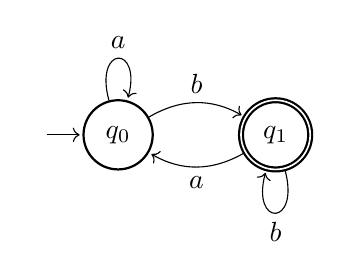
\begin{tikzpicture}[shorten >=1pt,on grid,auto]
        \coordinate (qs) at (0,0);
        \coordinate (qa) at (6,0);
        \node[state, initial] (q0) at (2,0) {$q_0$};
        \node[state, accepting] (q1) at (4,0) {$q_1$};
        \path[->]
            (q0) edge [loop above] node {$a$} ()
                 edge [bend left] node {$b$} (q1)
            (q1) edge [bend left] node {$a$} (q0)
                 edge [loop below] node {$b$} ();
    \end{tikzpicture}
    \end{center}
    \vspace*{1cm}
    \begin{center}
    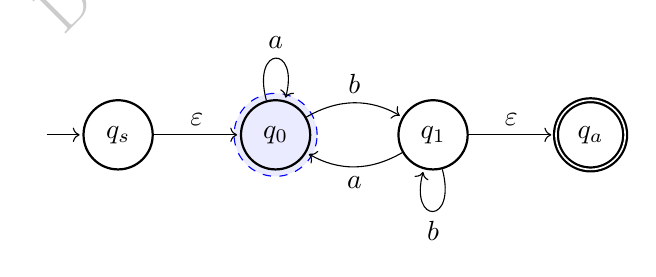
\begin{tikzpicture}[shorten >=1pt,on grid,auto]
        \node[state, initial] (qs) at (0,0) {$q_s$};
        \node[state] (q0) at (2,0) {$q_0$};
        \node[state] (q1) at (4,0) {$q_1$};
        \node[state, accepting] (qa) at (6,0) {$q_a$};

        \begin{pgfonlayer}{background}
            \draw[draw=blue,dashed,fill=blue!8] (q0) circle (15pt);
        \end{pgfonlayer}
            
        \path[->]
            (qs) edge node {$\varepsilon$} (q0)
            (q0) edge [loop above] node {$a$} ()
                 edge [bend left] node {$b$} (q1)
            (q1) edge [bend left] node {$a$} (q0)
                 edge [loop below] node {$b$} ()
                 edge node {$\varepsilon$} (qa);
    \end{tikzpicture}
    \end{center}
    \vspace*{1cm}
    \begin{center}
    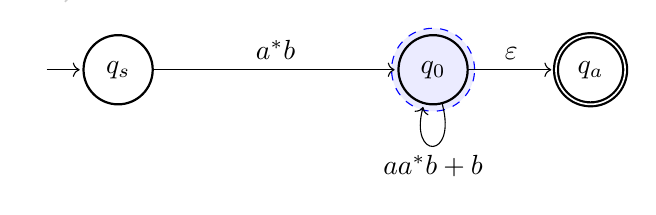
\begin{tikzpicture}[shorten >=1pt,on grid,auto]
        \node[state, initial] (qs) at (0,0) {$q_s$};
        \node[state] (q1) at (4,0) {$q_0$};
        \node[state, accepting] (qa) at (6,0) {$q_a$};

        \begin{pgfonlayer}{background}
            \draw[draw=blue,dashed,fill=blue!8] (q1) circle (15pt);
        \end{pgfonlayer}
            
        \path[->]
            (qs) edge node {$a^\ast b$} (q1)
            (q1) edge [loop below] node {$aa^\ast b+b$} ()
                 edge node {$\varepsilon$} (qa);
    \end{tikzpicture}
    \end{center}
    \vspace*{1cm}
    \begin{center}
    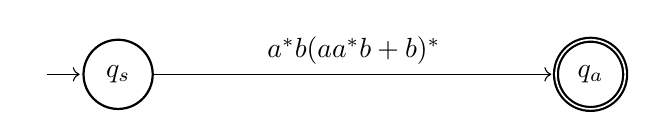
\begin{tikzpicture}[shorten >=1pt,on grid,auto]
        \node[state, initial] (qs) at (0,0) {$q_s$};
        \node[state, accepting] (qa) at (6,0) {$q_a$};

        \path[->]
            (qs) edge node {$a^\ast b(aa^\ast b+b)^\ast$} (qa);
    \end{tikzpicture}
    \end{center}
    So another regular expression equivalent to the original DFA is given by $a^\ast b(aa^\ast b+b)^\ast$.
\end{enumerate}


Recall that two states $q,q'$ of a DFA $M=(Q,\Sigma,\delta,q_0,F)$ are equivalent if the languages $L_q=L(M_q)$ and $L_{q'}=L(M_{q'})$ defined by the DFA $M_q=(Q,\Sigma,\delta,q,F)$ and $M_{q'}=(Q,\Sigma,q',\delta,F)$ that have initial states replaced by $q$ and $q'$ respectively, are equal.

\begin{enumerate}
    \item[$(iii)$] By induction on $|s|$. Let $q,q'$ be bisimilar.
    
    For $s=\varepsilon$, $q\in F$ if and only if $q'\in F$ by acceptance agreement of bisimilar states, so $\varepsilon\in L_q$ if and only if $\varepsilon\in L_{q'}$.

    Otherwise, suppose $s=aw$ with $w\in\Sigma^\ast$ and $a\in\Sigma$. By step correspondence, $\bigl\langle\delta(q,a),\delta(q',a)\bigr\rangle\in R$, and by the induction hypothesis, $w\in L_{\delta(q,a)}$ if and only if $w\in L_{\delta(q',a)}$, so $aw\in L_q$ if and only if $aw\in L_{q'}$.
\end{enumerate}




















\newpage

\section{Sheet 3}

\begin{questionbox}{$Q1$}
    Give context-free grammars that generate the following languages over the alphabet $\Sigma=\{0,1\}$:
    \begin{enumerate}
        \item[$(i)$] $L_1=\{w\mid w\text{ contains at least three occurences of }1\}$;
        
        \item[$(ii)$] $L_2=\{w\mid w\text{ starts and ends with the same symbol}\}$;
        
        \item[$(iii)$] $L_3=\{w\mid |w|\text{ is odd and its middle symbol is }0\}$;

        \item[$(iv)$] $L_4=\varnothing$;

        \item[$(v)$] $L_5=\{\varepsilon\}$.
    \end{enumerate}
\end{questionbox}

\bigskip

\begin{enumerate}
    \item[$(i)$] We need three occurences of $1$, and anything can go between or around them, so we can just immediately insert $A1A1A1A$, where $A$ generates $(0+1)^\ast$:
    \begin{align*}
        S&\longrightarrow A1A1A1A\\
        A&\longrightarrow AA\mid0\mid1\mid\varepsilon
    \end{align*}
    The production for $A$ can also be written linearly:
    \begin{equation*}
        A\longrightarrow0A\mid 1A\mid\varepsilon
    \end{equation*}
    
    \item[$(ii)$] We proceed similarly, immediately inserting the required matching pair of symbols (or taking care of edge cases like singletons and the empty word), and allow arbitrary expansion on the inside:
    \begin{align*}
        S&\longrightarrow 0A0\mid 1A1\mid0\mid1\mid\varepsilon\\
        A&\longrightarrow AA\mid0\mid1\mid\varepsilon
    \end{align*}

    \item[$(iii)$]\hspace*{1cm}
    \begin{align*}
        S&\longrightarrow ASA\mid0\\
        A&\longrightarrow0\mid1
    \end{align*}

    \item[$(iv)$] Any set of productions with no terminals will work:
    \begin{equation*}
        S\longrightarrow S
    \end{equation*}

    \item[$(v)$] \hspace*{1cm}
    \begin{equation*}
        S\longrightarrow\varepsilon
    \end{equation*}
\end{enumerate}
















\begin{questionbox}{$Q2$}
    Give context-free grammars equivalent to the following NFA:
    \begin{enumerate}
        \item[$(i)$]\hspace*{1cm}
        \begin{center}
            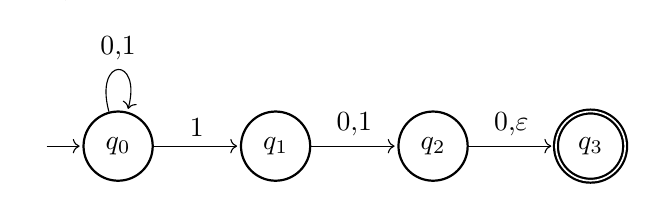
\begin{tikzpicture}[shorten >=1pt,node distance=2cm,on grid,auto]
                \node[state, initial] (q0) {$q_0$};
                \node[state] (q1) [right=of q0] {$q_1$};
                \node[state] (q2) [right=of q1] {$q_2$};
                \node[state, accepting] (q3) [right=of q2] {$q_3$};
                \path[->]
                    (q0) edge node {$1$} (q1)
                         edge [loop above] node {$0,1$} ()
                    (q1) edge node {$0,1$} (q2)
                    (q2) edge node {$0,\varepsilon$} (q3);
            \end{tikzpicture}
        \end{center}
        
        \item[$(ii)$]\hspace*{1cm}
        \begin{center}
            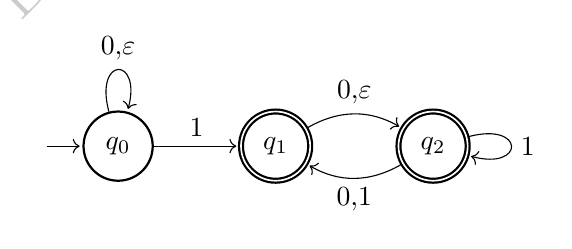
\begin{tikzpicture}[shorten >=1pt,node distance=2cm,on grid,auto]
                \node[state, initial] (q0) {$q_0$};
                \node[state, accepting] (q1) [right=of q0] {$q_1$};
                \node[state, accepting] (q2) [right=of q1] {$q_2$};
                \path[->]
                    (q0) edge node {$1$} (q1)
                         edge [loop above] node {$0,\varepsilon$} ()
                    (q1) edge [bend left] node {$0,\varepsilon$} (q2)
                    (q2) edge [bend left] node {$0,1$} (q1)
                         edge [loop right] node {$1$} ();
            \end{tikzpicture}
        \end{center}
    \end{enumerate}
\end{questionbox}

\bigskip

We can convert NFA to CFGs by interpreting states as non-terminals, and transitions as right-linear production rules. That is, taking a transition
\begin{center}
    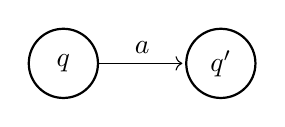
\begin{tikzpicture}[shorten >=1pt,node distance=2cm,on grid,auto]
        \node[state] (q0) {$q$};
        \node[state] (q1) [right=of q0] {$q'$};
        \path[->]
            (q0) edge node {$a$} (q1);
    \end{tikzpicture}
\end{center}
corresponds to adding a new terminal symbol $a$ to the left and replacing the non-terminal $Q$ with a new non-terminal $Q'$
\begin{equation*}
    Q\longrightarrow aQ'
\end{equation*}
and accepting states $q_a$ correspond to productions of the shape
\begin{equation*}
    Q_a\longrightarrow\varepsilon
\end{equation*}

\begin{enumerate}
    \item[$(i)$]\hspace*{1cm}
    \begin{align*}
        S&\longrightarrow Q_0\\
        Q_0&\longrightarrow0Q_0\mid 1Q_0\mid 1Q_1\\
        Q_1&\longrightarrow0Q_2\mid 1Q_2\\
        Q_2&\longrightarrow0Q_3\mid Q_3\\
        Q_3&\longrightarrow\varepsilon
    \end{align*}
    
    \item[$(ii)$]\hspace*{1cm}
    \begin{align*}
        S&\longrightarrow Q_0\\
        Q_0&\longrightarrow0Q_0\mid Q_0\mid 1Q_1\\
        Q_1&\longrightarrow\varepsilon\mid0Q_2\\
        Q_2&\longrightarrow\varepsilon\mid1Q_2\mid0Q_1\mid1Q_1\\
    \end{align*}
\end{enumerate}







\begin{questionbox}{$Q3$}
    Give context-free grammars equivalent to the following NFA:
    \begin{enumerate}
        \item[$(i)$] $0^\ast10^\ast$

        \item[$(ii)$] $1\cup0^\ast\emptyset$

        \item[$(iii)$] $(01^+)^+$
    \end{enumerate}
\end{questionbox}

\bigskip

\begin{enumerate}
    \item[$(i)$]\hspace*{1cm}
    \begin{align*}
        S&\longrightarrow Z1Z\\
        Z&\longrightarrow\varepsilon\mid0Z
    \end{align*}
    
    \item[$(ii)$] The symbol $\emptyset$ matches nothing, so $0^\ast\emptyset=\emptyset$ and $1\cup\emptyset=1$, so:
    \begin{equation*}
        S\longrightarrow1
    \end{equation*}

    \item[$(iii)$] Recall that $a^+=aa^\ast$. That is, $a^+$ matches one or more copies of $a$.
    \begin{align*}
        S&\longrightarrow0A\mid0AS\\
        A&\longrightarrow1\mid1A
    \end{align*}
\end{enumerate}








\begin{questionbox}{$Q4$}
    Provide an equivalent PDA for the language generated by the grammar $G=(V,\Sigma,R,E)$ with alphabet $\Sigma=\bigl\{a,\,(,\,),\times,+\bigr\}$, non-terminals $V=\{E,T,F\}$, and productions
    \begin{equation*}
        R=\left\{\begin{aligned}
            E&\longrightarrow E+T\mid T\\
            T&\longrightarrow T\times F\mid F\\
            F&\longrightarrow (E)\mid a
        \end{aligned}\right\}
    \end{equation*}
\end{questionbox}

\bigskip


We can simulate a leftmost derivation of the grammar on a PDA by using the stack to represent the current sentential state.
\begin{enumerate}
    \item First, push $S\$$ on to the stack to initialise the derivation at $S$, and using $\$$ for empty-stack detection, and move to a processing state.
    \item For each production $A\rightarrow\beta$ in $R$, add an operation $\varepsilon,A\rightarrow\beta$, corresponding to (non-deterministically) applying a production rule for $A$.
    \item For each terminal $a\in\Sigma$, add an operation $a,a\rightarrow\varepsilon$, allowing the PDA to match terminals produced by the grammar against the input string.
    \item Once the top of the stack is $\$$, corresponding to a completed derivation, move to an accept state.
\end{enumerate}
\begin{center}
    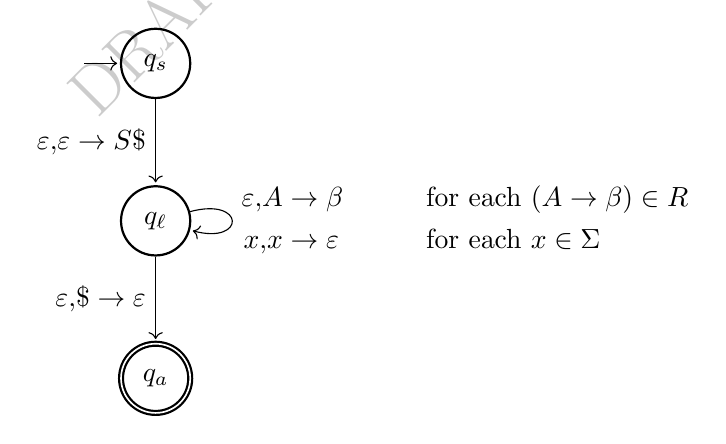
\begin{tikzpicture}[shorten >=1pt,node distance=2cm,on grid,auto] 
        \node[state, initial] (q_s) {$q_s$}; 
        \node[state] (q_l) [below=of q_s] {$q_\ell$}; 
        \node[state, accepting] (q_a) [below=of q_l] {$q_a$}; 
        \path[->] 
        (q_s) edge [swap]       node {$\varepsilon,\varepsilon\rightarrow S\$$} (q_l)
        (q_l) edge [swap]       node {$\varepsilon,\$\rightarrow\varepsilon$} (q_a)
              edge [loop right] node {$\begin{aligned}\varepsilon,A&\rightarrow\beta\qquad&&\text{for each }(A\rightarrow\beta)\in R\\x,x&\rightarrow\varepsilon\qquad&&\text{for each }x\in\Sigma\end{aligned}$} ();
    \end{tikzpicture}
\end{center}
Note that we are implicitly using more than just $3$ states when pushing multiple symbols to the stack: for the final PDA, any rules that produce multiple symbols can be expanded into multiple states that push the symbols on to the stack one at a time. Note that the symbols must be pushed on to the stack in reverse order, as stacks are first-in-last-out.

For this question, we have:
\begin{center}
    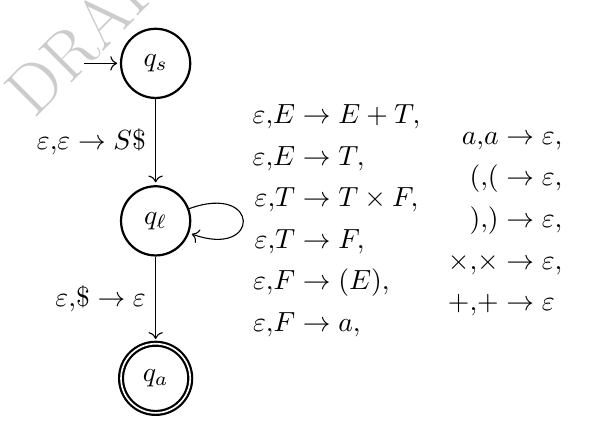
\begin{tikzpicture}[shorten >=1pt,node distance=2cm,on grid,auto] 
        \node[state, initial] (q_s) {$q_s$}; 
        \node[state] (q_l) [below=of q_s] {$q_\ell$}; 
        \node[state, accepting] (q_a) [below=of q_l] {$q_a$}; 
        \path[->] 
        (q_s) edge [swap]       node {$\varepsilon,\varepsilon\rightarrow S\$$} (q_l)
        (q_l) edge [swap]       node {$\varepsilon,\$\rightarrow\varepsilon$} (q_a)
              edge [out=20,in=340,looseness=2,loop] node {$
                \begin{aligned}
                    \varepsilon,E&\rightarrow E+T,\\
                    \varepsilon,E&\rightarrow T,\\
                    \varepsilon,T&\rightarrow T\times F,\\
                    \varepsilon,T&\rightarrow F,\\
                    \varepsilon,F&\rightarrow(E),\\
                    \varepsilon,F&\rightarrow a,
                \end{aligned}\quad\begin{aligned}
                    a,a&\rightarrow\varepsilon,\\
                    (,(&\rightarrow\varepsilon,\\
                    ),)&\rightarrow\varepsilon,\\
                    \times,\times&\rightarrow\varepsilon,\\
                    +,+&\rightarrow\varepsilon
                \end{aligned}$} ();
    \end{tikzpicture}
\end{center}


Expanding this out in full:



\begin{center}
    \begin{tikzpicture}[shorten >=1pt,node distance=2.5cm,on grid,auto]
        \node[state, initial] (qs) {$q_{s_0}$};
        \node[state] (qt) [right=of qs]{$q_{s_1}$};

        \node[state] (ql) [below=of qt]{$q_\ell$};
        \node[state, accepting] (qa) [below=of ql] {$q_a$};

        \node[state] (r0) [above right=4.5cm of ql] {$r_0$};
        \node[state] (r1) [right=of r0] {$r_1$};

        \node[state] (s0) [right=4.5cm of ql] {$s_0$};
        \node[state] (s1) [right=of s0] {$s_1$};

        \node[state] (t0) [below right=4.5cm of ql] {$t_0$};
        \node[state] (t1) [right=of t0] {$t_1$};

        
        \path[->]
            (qs) edge node {$\varepsilon,\varepsilon\rightarrow\$$} (qt)
            (qt) edge [near start, swap] node {$\varepsilon,\varepsilon\rightarrow S$} (ql)
            
            (ql) edge [near end] node {$\varepsilon,E\rightarrow T$} (r0)
                 edge node {$\varepsilon,T\rightarrow F$} (s0)
                 edge [near end, swap] node {$\varepsilon,F\rightarrow)$} (t0)
                 edge [near end, swap] node {$\varepsilon,\$\rightarrow\varepsilon$} (qa)
                 edge [out=160,in=200,looseness=2,loop] node [left] {$
                \begin{aligned}
                    \varepsilon,E&\rightarrow T,\\
                    \varepsilon,T&\rightarrow F,\\
                    \varepsilon,F&\rightarrow a,\\
                    a,a&\rightarrow\varepsilon,
                \end{aligned}\quad\begin{aligned}
                    (,(&\rightarrow\varepsilon,\\
                    ),)&\rightarrow\varepsilon,\\
                    \times,\times&\rightarrow\varepsilon,\\
                    +,+&\rightarrow\varepsilon
                \end{aligned}$} ()

            (r0) edge node {$\varepsilon,\varepsilon\rightarrow+$} (r1)
            (r1) edge [near start] node {$\varepsilon,\varepsilon\rightarrow E$} (ql)

            (s0) edge node {$\varepsilon,\varepsilon\rightarrow\times$} (s1)
            (s1) edge [near start, out=205,in=345] node {$\varepsilon,\varepsilon\rightarrow T$} (ql)

            (t0) edge [swap] node {$\varepsilon,\varepsilon\rightarrow E$} (t1)
            (t1) edge [near start, swap] node {$\varepsilon,\varepsilon\rightarrow($} (ql);

        \node (r) [right=20pt of r1,anchor=west] {$\textcolor{blue}{\varepsilon,E\rightarrow E+T}$};
        \node (s) [right=20pt of s1,anchor=west] {$\textcolor{cyan}{\varepsilon,T\rightarrow T\times F}$};
        \node (t) [right=20pt of t1,anchor=west] {$\textcolor{purple}{\varepsilon,F\rightarrow(E)}$};
        
        \begin{pgfonlayer}{background}
            \node (box) [draw=blue, fill=blue!8, fit=(r0) (r1), inner sep=5pt, rounded corners] {};
            \node (box2) [draw=cyan, fill=cyan!8, fit=(s0) (s1), inner sep=5pt, rounded corners] {};
            \node (box3) [draw=purple, fill=purple!8, fit=(t0) (t1), inner sep=5pt, rounded corners] {};
        \end{pgfonlayer}
    \end{tikzpicture}
\end{center}













\begin{questionbox}{$Q5$}
    Construct a PDA for each of the following languages over the alphaber $\Sigma=\{0,1\}$:
    \begin{enumerate}
        \item[$(i)$] $L_1=\{w\mid w\text{ contains at least three occurences of }1\}$;
        
        \item[$(ii)$] $L_2=\{w\mid w\text{ starts and ends with the same symbol}\}$;
        
        \item[$(iii)$] $L_3=\{w\mid |w|\text{ is odd and its middle symbol is }0\}$.
    \end{enumerate}
\end{questionbox}

\bigskip

\begin{enumerate}
    \item[$(i)$] This language is regular:
    \begin{center}
        \begin{tikzpicture}[shorten >=1pt,node distance=2cm,on grid,auto]
            \node[state, initial] (q0) {$q_0$};
            \node[state] (q1) [right=of q0] {$q_1$};
            \node[state] (q2) [right=of q1] {$q_2$};
            \node[state, accepting] (q3) [right=of q2] {$q_3$};
            \path[->]
                (q0) edge node {$1$} (q1)
                     edge [loop above] node {$0,1$} ()
                (q1) edge node {$1$} (q2)
                     edge [loop above] node {$0,1$} ()
                (q2) edge node {$1$} (q3)
                     edge [loop above] node {$0,1$} ()
                (q3) edge [loop above] node {$0,1$} ();
        \end{tikzpicture}
    \end{center}
    and every DFA is a PDA that happens to have all stack instructions $\varepsilon\rightarrow\varepsilon$.
    
    Alternatively, the stack can be used to count the number of $1$'s:
    \begin{center}
    \begin{tikzpicture}[shorten >=1pt,node distance=3cm,on grid,auto]
        \node[state, initial] (q0) {$q_0$};
        \node[state, accepting] (q1) [right=of q0] {$q_1$};
        \path[->]
            (q0) edge node {$1,\mathsf{2}\rightarrow\varepsilon$} (q1)
                 edge [loop above] node {$\begin{aligned}
                    0,\varepsilon&\rightarrow\varepsilon\\
                    1,\varepsilon&\rightarrow\mathsf{1}\\
                    1,\mathsf{1}&\rightarrow\mathsf{2}\\
                 \end{aligned}$} ()
            (q1) edge [loop above] node {$\begin{aligned}
                    0,\varepsilon&\rightarrow\varepsilon\\
                    1,\varepsilon&\rightarrow\varepsilon
                 \end{aligned}$} ();
    \end{tikzpicture}
    \end{center}
    
    \item[$(ii)$] $L_2$ is also regular. An NFA accepting $L_2$ is as follows:
    \begin{center}
    \begin{tikzpicture}[shorten >=1pt,node distance=2cm,on grid,auto]
        \node[state, initial, accepting] (q0) {$q_0$};
        \node[state, accepting] (q1) [above left=of q0] {$q_1$};
        \node[state, accepting] (q2) [below left=of q0] {$q_2$};
        \node[state] (q3) [above right=of q0] {$q_3$};
        \node[state] (q4) [below right=of q0] {$q_4$};
        \node[state, accepting] (q5) [below right=of q3] {$q_5$};

        \path[->]
            (q0) edge [swap] node {$1$} (q1)
                 edge node {$0$} (q2)
                 edge node {$1$} (q3)
                 edge [swap] node {$0$} (q4)
            (q3) edge node {$1$} (q5)
                 edge [loop above] node {$0,1$} ()
            (q4) edge [swap]node {$0$} (q5)
                 edge [loop below] node {$0,1$} ();
    \end{tikzpicture}
    \end{center}

    \item[$(iii)$] This language is not regular. The stack can again be used for counting: every time an input symbol is read, push the symbol $X$ on to the stack and use non-determinism to find where the middle $0$ is; then pop from the stack for each input symbol and accept on empty stack, ensuring there are the same number of symbols on each side of the $0$.
    \begin{center}
    \begin{tikzpicture}[shorten >=1pt,node distance=3cm,on grid,auto]
        \node[state, initial] (q0) {$q_0$};
        \node[state] (q1) [right=of q0] {$q_1$};
        \node[state] (q2) [right=of q1] {$q_2$};
        \node[state, accepting] (q3) [right=of q2] {$q_3$};
        \path[->]
            (q0) edge node {$\varepsilon,\varepsilon\rightarrow\$$} (q1)
            (q1) edge node {$1$} (q2)
                 edge [loop above] node {$\begin{aligned}
                0,\varepsilon&\rightarrow X\\
                1,\varepsilon&\rightarrow X
             \end{aligned}$} ()
            (q2) edge node {$\varepsilon,\$\rightarrow\varepsilon$} (q3)
                 edge [loop above] node {$\begin{aligned}
                0,X&\rightarrow\varepsilon\\
                1,X&\rightarrow\varepsilon
             \end{aligned}$} ();
    \end{tikzpicture}
    \end{center}
\end{enumerate}








\begin{questionbox}{$Q6$}
    Construct an equivalent PDA for the following NFA:
    \begin{center}
    \begin{tikzpicture}[shorten >=1pt,node distance=2cm,on grid,auto]
        \node[state, initial] (q0) {$q_0$};
        \node[state, accepting] (q1) [above right=of q0,xshift=1cm]{$q_1$};
        \node[state, accepting] (q2) [below right=of q0,xshift=1cm]{$q_2$};
        
        \path[->]
            (q0) edge node {$b$} (q1)
                 edge [out=345,in=135] node {$\varepsilon$} (q2)
            (q1) edge node {$a,b$} (q2)
                 edge [loop above] node {$a$} ()
            (q2) edge [in=315,out=165] node {$a$} (q0);
    \end{tikzpicture}
    \end{center}
\end{questionbox}

\bigskip

Every NFA is a PDA that just doesn't use its stack.
\begin{center}
\begin{tikzpicture}[shorten >=1pt,node distance=2cm,on grid,auto]
    \node[state, initial] (q0) {$q_0$};
    \node[state, accepting] (q1) [above right=of q0,xshift=1cm]{$q_1$};
    \node[state, accepting] (q2) [below right=of q0,xshift=1cm]{$q_2$};
    
    \path[->]
        (q0) edge node {$b,\varepsilon\rightarrow\varepsilon$} (q1)
             edge [near start, out=345,in=135] node {$\varepsilon,\varepsilon\rightarrow\varepsilon$} (q2)
        (q1) edge node {$\begin{aligned}
            a,\varepsilon&\rightarrow\varepsilon\\
            b,\varepsilon&\rightarrow\varepsilon
        \end{aligned}$} (q2)
             edge [loop above] node {$a,\varepsilon\rightarrow\varepsilon$} ()
        (q2) edge [in=315,out=165] node {$a,\varepsilon\rightarrow\varepsilon$} (q0);
\end{tikzpicture}
\end{center}











\begin{questionbox}{$Q7$}
    Consider the following three languages over the alphabet $\Sigma=\{a,b,c\}$:
    \begin{align*}
        L_1&=\{a^ib^jc^k\mid i,j,k\geq0,i=j=k\}\\
        L_2&=\{a^ib^jc^k\mid i,j,k\geq0,i=j\phantom{{}=k}\}\\
        L_3&=\{a^ib^jc^k\mid i,j,k\geq0,\phantom{i={}}j=k\}
    \end{align*}
    \begin{enumerate}
        \item[$(i)$] Determine and prove which two are context-free.
        
        \item[$(ii)$] Prove that the third language is not context-free.
    
        \item[$(iii)$] Hence conclude that the class of context-free languages is not closed under intersection.
    \end{enumerate}
\end{questionbox}

\bigskip

\begin{enumerate}
    \item[$(i)$] Using a stack, we can compare two things for equality, so $L_2$ and $L_3$ are context-free. Context-free grammars that generate them are as follows:
    \begin{equation*}
        \begin{aligned}
            L_2:\quad S&\rightarrow XC\\
            C&\rightarrow\varepsilon\mid cC\\
            X&\rightarrow\varepsilon\mid aXb\\
        \end{aligned}\qquad\qquad
        \begin{aligned}
            L_3:\quad S&\rightarrow AX\\
            A&\rightarrow\varepsilon\mid aA\\
            X&\rightarrow\varepsilon\mid bXc\\
        \end{aligned}
    \end{equation*}
\end{enumerate}


Recall the pumping lemma for regular languages:
\begin{lemma*}[Pumping Lemma]
    Let $L$ be a regular language. Then, there exists an integer $p\geq 1$ (the \textit{pumping length}), such that for every string $s\in L$ with length $|s|\geq p$, there exists a decomposition $s=x\cdot y\cdot z$ such that
    \begin{itemize}
        \item $|y|\geq1$;
        \item $|xy|\leq p$;
        \item for all $n\geq0$, $x\cdot y^n\cdot z\in L$.
    \end{itemize}
\end{lemma*}
The intuition was that if an input string is too long, then it must loop somewhere inside the DFA.

A similar result holds for context-free languages, in that if a derived string is too long, it must repeat a variable somewhere in its parse tree. Similarly to before we can generate an infinite set of strings in the language by pumping this repeated variable:

Suppose we repeat a variable $R$, and that the derivation between the first and second $R$ yields a string that starts with a string $v$ and ends with a string $y$.
\begin{center}
    \begin{tikzpicture}
        \begin{scope}
            \clip (-3,0.25) rectangle (3,3.2);
            \draw
                (0,3) -- +(-50:4)
                (0,2) -- +(-50:4)
                (0,1) -- +(-50:4)
                (0,3) -- +(230:4)
                (0,2) -- +(230:4)
                (0,1) -- +(230:4);
            \draw[thin, gray!30]
                (0,2.75) -- +(-50:4)
                (0,2.50) -- +(-50:4)
                (0,2.25) -- +(-50:4)
                (0,1.75) -- +(-50:4)
                (0,1.50) -- +(-50:4)
                (0,1.25) -- +(-50:4)
                (0,2.75) -- +(230:4)
                (0,2.50) -- +(230:4)
                (0,2.25) -- +(230:4)
                (0,1.75) -- +(230:4)
                (0,1.50) -- +(230:4)
                (0,1.25) -- +(230:4);

            \draw[dash pattern=on 2pt off 1pt]
                (0,3) -- (0,1);
        \end{scope}
        
        \draw (-2.3075,0.25) -- (2.3075,0.25);

        \draw
            (-2,0) node {$u$}
            (-1,0) node {$v$}
            (0,0)  node {$x$}
            (1,0)  node {$y$}
            (2,0)  node {$z$};

        \filldraw[draw=none, fill=white]
            (0,3) circle (5.5pt) node {$T$}
            (0,2) circle (5.5pt) node {$R$}
            (0,1) circle (5.5pt) node {$R$};
    \end{tikzpicture}
\end{center}
Then, if we repeat $R$ again, the derivation will repeat $v$ and $y$:
\begin{center}
    \begin{tikzpicture}
        \begin{scope}
            \clip
                (-3,0.25)
             -- (-0.75,0.25)
             -- +(230:2)
             -- ($(0.75,0.25)+(-50:2)$)
             -- (0.75,0.25)
             -- (3,0.25)
             -- (3,3.2)
             -- (-3,3.2)
             -- cycle;
            \clip (-3,-0.75) rectangle (3,3.2);
            \draw
                (0,3) -- +(-50:4)
                (0,2) -- +(-50:4)
                (0,1) -- +(-50:4)
                (0,0) -- +(-50:4)
                (0,3) -- +(230:4)
                (0,2) -- +(230:4)
                (0,1) -- +(230:4)
                (0,0) -- +(230:4);
            \draw[thin, gray!30]
                (0,2.75) -- +(-50:4)
                (0,2.50) -- +(-50:4)
                (0,2.25) -- +(-50:4)
                (0,1.75) -- +(-50:4)
                (0,1.50) -- +(-50:4)
                (0,1.25) -- +(-50:4)
                (0,0.75) -- +(-50:4)
                (0,0.50) -- +(-50:4)
                (0,0.25) -- +(-50:4)
                (0,2.75) -- +(230:4)
                (0,2.50) -- +(230:4)
                (0,2.25) -- +(230:4)
                (0,1.75) -- +(230:4)
                (0,1.50) -- +(230:4)
                (0,1.25) -- +(230:4)
                (0,0.75) -- +(230:4)
                (0,0.50) -- +(230:4)
                (0,0.25) -- +(230:4);
                
            \draw[dash pattern=on 2pt off 1pt]
                (0,3) -- (0,0);
        \end{scope}
        
        \draw
            (-2.3075,0.25) -- (-0.629,0.25)
            (-1.468,-0.75) -- (1.468,-0.75)
            (0.629,0.25) -- (2.3075,0.25);

        \draw
            (-2,0)  node {$u$}
            (-1,-1) node {$v$}
            (-1.25,0)  node {$v$}
            (0,-1)  node {$x$}
            (1,-1)  node {$y$}
            (1.25,0)   node {$y$}
            (2,0)   node {$z$};

        \filldraw[draw=none, fill=white]
            (0,3) circle (5.5pt) node {$T$}
            (0,2) circle (5.5pt) node {$R$}
            (0,1) circle (5.5pt) node {$R$}
            (0,0) circle (5.5pt) node {$R$};
    \end{tikzpicture}
\end{center}
We can also remove the repeated $R$:
\begin{center}
    \begin{tikzpicture}
        \begin{scope}
            \clip (-3,0.25) rectangle (3,3.2);
            \draw
                (0,3) -- +(-50:4)
                (0,2) -- +(-50:4)
                (0,3) -- +(230:4)
                (0,2) -- +(230:4);
            \draw[thin, gray!30]
                (0,2.75) -- +(-50:4)
                (0,2.50) -- +(-50:4)
                (0,2.25) -- +(-50:4)
                (0,2.75) -- +(230:4)
                (0,2.50) -- +(230:4)
                (0,2.25) -- +(230:4);
                
            \draw[dash pattern=on 2pt off 1pt]
                (0,3) -- (0,2);
        \end{scope}
        
        \draw
            (-2.3075,0.25) -- (-1.468,0.25)
            (-0.629,1.25) -- (0.629,1.25)
            (1.468,0.25) -- (2.3075,0.25);

        \draw
            (-2,0)  node {$u$}
            (0,1)  node {$x$}
            (2,0)   node {$z$};

        \filldraw[draw=none, fill=white]
            (0,3) circle (5.5pt) node {$T$}
            (0,2) circle (5.5pt) node {$R$};
    \end{tikzpicture}
\end{center}


\begin{lemma}[Pumping Lemma]
    Let $L$ be a context free language. Then, there exists an integer $p\geq1$ (the pumping length) such that for every string $s\in L$ with length $|s|\geq p$, there exists a decomposition $s=u\cdot v\cdot x\cdot y\cdot z$ such that
    \begin{itemize}
        \item $|vy|\geq 1$;
        \item $|vxy|\leq p$;
        \item for all $n\geq0$, $u\cdot v^n\cdot x\cdot y^n\cdot z\in L$.
    \end{itemize}
\end{lemma}
\begin{proof}
    Let $G=(V,\Sigma,R,S)$ be a CFG, and suppose that the length of the longest string in the right side of a production rule in $R$ is $b$. Then, any node in a parse tree yielding a string in $L(G)$ has at most $b$ children. If the height of the tree is $h$, then it has at most $b^h$ leaves, as each layer can only have $b$ times as many nodes as the previous layer.

    How long must a string be such that a variable is repeated on some root to leaf path of any parse tree of this string?

    We claim that $p\coloneqq b^{|V|+1}$ is sufficient. Indeed, the parse tree of such a word must have $b^{|V|+1}$ leaves, so the tree must have height at least $|V|+1$. But, there are only $|V|$ variables, so one must repeat.

    Take the smallest parse tree for the string $w=uvxyz$. If $|vy|\not\geq1$, then $v=y=\varepsilon$, and the section of the parse tree between the two $R$s don't contribute anything, so $w=uxz$, and we have an even smaller parse tree for $w$, contradicting the minimality of the first tree.
    \begin{center}
        \begin{tikzpicture}
            \begin{scope}
                \clip (-3,0.25) rectangle (3,3.2);
                \draw
                    (0,3) -- +(-50:4)
                    (0,2) -- +(-50:4)
                    (0,1) -- +(-50:4)
                    (0,3) -- +(230:4)
                    (0,2) -- +(230:4)
                    (0,1) -- +(230:4);
                \draw[thin, gray!30]
                    (0,2.75) -- +(-50:4)
                    (0,2.50) -- +(-50:4)
                    (0,2.25) -- +(-50:4)
                    (0,1.75) -- +(-50:4)
                    (0,1.50) -- +(-50:4)
                    (0,1.25) -- +(-50:4)
                    (0,2.75) -- +(230:4)
                    (0,2.50) -- +(230:4)
                    (0,2.25) -- +(230:4)
                    (0,1.75) -- +(230:4)
                    (0,1.50) -- +(230:4)
                    (0,1.25) -- +(230:4);
    
                \draw[dash pattern=on 2pt off 1pt]
                    (0,3) -- (0,1);
            \end{scope}
            
            \draw (-2.3075,0.25) -- (2.3075,0.25);
    
            \draw
                (-2,0) node {$u$}
                (-1,0) node {$\varepsilon$}
                (0,0)  node {$x$}
                (1,0)  node {$\varepsilon$}
                (2,0)  node {$z$};
    
            \filldraw[draw=none, fill=white]
                (0,3) circle (5.5pt) node {$T$}
                (0,2) circle (5.5pt) node {$R$}
                (0,1) circle (5.5pt) node {$R$};
        \end{tikzpicture}
        \hspace*{2cm}
        \begin{tikzpicture}
            \begin{scope}
                \clip (-3,0.25) rectangle (3,3.2);
                \draw
                    (0,3) -- +(-50:4)
                    (0,2) -- +(-50:4)
                    (0,3) -- +(230:4)
                    (0,2) -- +(230:4);
                \draw[thin, gray!30]
                    (0,2.75) -- +(-50:4)
                    (0,2.50) -- +(-50:4)
                    (0,2.25) -- +(-50:4)
                    (0,2.75) -- +(230:4)
                    (0,2.50) -- +(230:4)
                    (0,2.25) -- +(230:4);
                    
                \draw[dash pattern=on 2pt off 1pt]
                    (0,3) -- (0,2);
            \end{scope}
            
            \draw
                (-2.3075,0.25) -- (-1.468,0.25)
                (-0.629,1.25) -- (0.629,1.25)
                (1.468,0.25) -- (2.3075,0.25);
    
            \draw
                (-2,0)  node {$u$}
                (0,1)  node {$x$}
                (2,0)   node {$z$};
    
            \filldraw[draw=none, fill=white]
                (0,3) circle (5.5pt) node {$T$}
                (0,2) circle (5.5pt) node {$R$};
        \end{tikzpicture}
    \end{center}
    If $|vxy|>p$, then the subtree rooted at the first $R$ is itself long enough to have a repeated variable on a root to leaf path. So, we can split $x$ into $x=u'x'y'$, so $w=(uv)v'x'y'(yz)$, which is still of the required form, but the middle substring has now decreased in length. We can then repeat this process until the middle substring has length at most $p$.
\end{proof}





\begin{enumerate}
    \item[$(ii)$] Suppose $L_1$ is context-free and $p$ be its pumping length. Consider the string $s=a^pb^pc^p$ and let $s=uvxyz$ be a decomposition with $|vy|\geq1$ and $|vxy|\leq p$. Since $|vy|\geq1$, they can't both be empty, and since $|vxy|\leq p$, $vxy$ contains at most $2$ of the symbols. Pumping $vxy$ zero times then reduces the number of only two of the symbols.

    \item[$(iii)$] $L_1=L_2\cap L_3$; $L_2$ and $L_3$ are context-free, but $L_1$ is not. Note that this also proves that context-free languages are not closed under complementation since intersections can be constructed from unions and complements:
    \begin{equation*}
        A\cap B=(A^c\cup B^c)^c
    \end{equation*}
\end{enumerate}











\begin{questionbox}{$Q8$}
    Consider the language
    \begin{equation*}
        L_4=\bigl\{u\#w\mid u,w\in\{0,1\}^\ast,u\text{ is a prefix of }w\bigr\}
    \end{equation*}
    \begin{enumerate}
        \item[$(i)$] Find some examples of strings that belong to $L_4$ and some non-examples that do not.
        
        \item[$(ii)$] Prove or disprove that $L_4$ is context-free.
    \end{enumerate}
\end{questionbox}

\bigskip

\begin{enumerate}
    \item[$(i)$] $\#,\#0,\#11,0\#01,11\#1100,\ldots\in L_4$ and $\varepsilon,01,0\#,1\#0,11\#1011,\ldots\notin L_4$.
    
    \item[$(ii)$] Suppose that $L_4$ is context free and let $p$ be its pumping length. Consider the string $s=0^p1^p\#0^p1^p$ and let $s=uvxyz$ be a decomposition satisfying the hypotheses of the pumping lemma. Since $|vy|\geq1$, they cannot both be empty.
    \begin{itemize}
        \item If $v$ or $y$ contains $\#$, then pumping down removes the $\#$ from the string;
        \item If $v$ and $y$ are both to the left of $\#$, then pumping upwards makes the left substring longer than the right substring, so it cannot be a prefix;
        \item If $v$ and $y$ are both to the right of $\#$, then pumping downwards makes the right substring shorter than the left substring;
        \item Otherwise, $v$ and $y$ are on either side of the $\#$. Since $|vxy|\leq p$, if $v$ is non-empty, then it contains only $1$'s; and if $y$ is non-empty it contains only $0$'s. Then, pumping upwards increases the number of $1$'s on the left and/or reduces the number of $0$'s on the right, so the left substring cannot be a prefix.
    \end{itemize}
\end{enumerate}






\newpage

\section{Sheet 4}




\begin{questionbox}{$Q1$}
    \begin{enumerate}
        \item[$(i)$] Can a Turing machine ever write the blank symbol $\sqcup$ on its tape?
        
        \item[$(ii)$] Can the tape alphabet $\Gamma$ be equal to the input alphabet $\Sigma$?
    
        \item[$(iii)$] Can the head of a Turing machine ever stay on the same cell for two subsequent steps of a computation?
    
        \item[$(iv)$] Can the state set of a Turing machine consist of only a single state?
    \end{enumerate}
\end{questionbox}

\bigskip

\begin{enumerate}
    \item[$(i)$] Yes: by definition, the tape alphabet $\Gamma$ contains $\sqcup$, and the transition function $\delta:Q\times\Gamma\rightarrow Q\times\Gamma\times\{\mathsf{L},\mathsf{R}\}$ allows the machine to write any symbol from $\Gamma$ to the tape, including $\sqcup$.
    
    \item[$(ii)$] No: $\sqcup\in\Gamma\setminus\Sigma$.

    \item[$(iii)$] Yes: if the move instruction is $\mathsf{L}$ while the head is on the leftmost cell, the head does not move.

    \item[$(iv)$] No: $q_\text{accept}$ and $q_\text{reject}$ must be distinct.
\end{enumerate}


\begin{questionbox}{$Q2$}
    Some of the following definitions are correct and some wrong (and some are even pure nonsense). Mark the correct definitions and for the incorrect ones underline the part of the definition which is wrong and explain why.
    \begin{enumerate}
        \item[$(i)$] A language $L$ is recognisable if the language halts in the state $q_\text{acc}$ whenever $x\in L$.
        
        \item[$(ii)$] A language $L$ is recognisable if there exists a Turing machine $M$ such that $M$, given input $x$, halts in the state $q_\text{accept}$ if and only if $x\in L$.
    
        \item[$(iii)$] A language $L$ is recognisable if it halts in an accepting state $q_\text{accept}$ whenever $x\in L$.
    
        \item[$(iv)$] A language $L$ is recognisable if there exists a Turing machine $M$ which has a state $q_\text{accept}$ and is a member of $L$.
        
        \item[$(v)$] A language $L$ is recognisable if there exists a Turing machine $M$ such that for any given input $x$, the run on $x$ halts in the state $q_\text{accept}$ if $x\in L$ and either loops or halts in $q_\text{reject}$ if $x\notin L$.
        
        \item[$(vi)$] A language $L$ is recognisable if every Turing machine $M$, when run on a string $x$, halts in the state $q_\text{accept}$ if and only if $x\in L$.
    \end{enumerate}
\end{questionbox}

\bigskip

\begin{enumerate}
    \item[$(i)$] Wrong: ``A language $L$ is recognisable if \underline{the language halts} in the state $q_\text{acc}$ whenever $x\in L$.'' -- the language itself does not run/halt. Also, unbound variable $x$.
    
    \item[$(ii)$] Correct.

    \item[$(iii)$] Wrong: ``A language $L$ is recognisable if \underline{it halts} in an accepting state $q_\text{accept}$ whenever $x\in L$.'' -- same as above.

    \item[$(iv)$] Wrong: ``A language $L$ is recognisable if there exists a \underline{Turing machine} $M$ which has a state $q_\text{accept}$ and \underline{is a member of $L$}.'' -- Turing machines are not (in general) elements of a language, so this doesn't make sense for a general definition.

    \item[$(v)$] Correct.
    
    \item[$(vi)$] Wrong: ``A language $L$ is recognisable if \underline{every} Turing machine $M$, when run on a string $x$, halts in the state $q_\text{accept}$ if and only if $x\in L$.'' -- there only needs to exist a single Turing machine that halts on every string in $L$. (And since there exist Turing machines that recognise disjoint languages, no language satisfies this definition.)
\end{enumerate}.


\begin{questionbox}{$Q3$}
    Complete the definition below and be formally precise:
    \begin{quote}
        A language $L\subseteq\Sigma^\ast$ is decidable if and only if\ldots
    \end{quote}
\end{questionbox}

\bigskip

There are many equivalent definitions. Here are a few:

\begin{itemize}
    \item A language $L\subseteq\Sigma^\ast$ is decidable if and only if there exists a Turing machine $M$ such that $M$ halts on a string $x$ in $q_\text{accept}$ if and only if $x\in L$ and halts in $q_\text{reject}$ if and only if $x\notin L$.

    \item A language $L\subseteq\Sigma^\ast$ is decidable if and only if $L$ is recognisable and $\Sigma^\ast\setminus L$ is recognisable.\footnote{The class of Turing-decidable languages is also called the class of \textit{recursive} languages, denoted by $\textsf{R}$; and the class of Turing-recognisable languages is also called the class of \textit{recursively enumerable} languages, denoted by $\textsf{RE}$. This definition can then be phrased as $\textsf{R}=\textsf{RE}\cap\textsf{co-RE}$, where \textsf{co-RE} is the class of languages whose complements are recursively enumerable. These names stem from recursion theory and mathematical logic, which studies a different, but equivalent, model of computation known as \textit{general recursive functions}.}
    
    \item A language $L\subseteq\Sigma^\ast$ is decidable if and only if there exists two Turing machines; one that enumerates exactly the strings in $L$ in some order, and one that enumerates the strings in $\Sigma^\ast\setminus L$ in some order.
\end{itemize}






\begin{questionbox}{$Q4$}
    Consider the language
    \begin{equation*}
        L=\{a^nb^na^n\mid n\geq0\}
    \end{equation*}
    \begin{enumerate}
        \item[$(i)$] Prove that $L$ is not context-free.
        
        \item[$(ii)$] Draw a state diagram of a Turing machine that recognises $L$.
    
        \item[$(iii)$] Consider the input string $s=aabbaa$. Trace the sequence of configurations that $M$ enters when run on $w$.
    
        \item[$(iv)$] Does $M$ accept $w$?
    \end{enumerate}
\end{questionbox}

\bigskip

\begin{enumerate}
    \item[$(i)$] Suppose $L$ is context-free and let $p$ be its pumping length. Consider the string $s=a^pb^pa^p$ and let $s=uvxyz$ be a decomposition satisfying the hypotheses of the pumping lemma. Since $|vxy|\leq p$, $vxy$ is either contained in first two parts $a^pb^p$ or the last two parts $b^pa^p$. In either case, pumping the string only changes the number of symbols in two of the three parts.
    
    \item[$(ii)$]\hspace*{1cm}

    \begin{center}
    \begin{tikzpicture}[shorten >=1pt,node distance=3cm,on grid,auto]
        \node[state, initial] (q0) {$q_0$};
        \node[state] (qr) [above right=of q0] {$q_\text{rej}$};
        \node[state] (qa) [below right=of qr] {$q_\text{acc}$};
        \node[state] (q1) [above left=of qr] {$q_1$};
        \node[state] (q2) [above right=of q1] {$q_2$};
        \node[state] (q3) [below right=of q2] {$q_3$};
        \node[state] (q4) [below right=of q3] {$q_4$};
        \node[state] (q5) [below right=of q0] {$q_5$};
        \node[state] (q6) [below left=of q1] {$q_6$};

        \path[->]
            (q0) edge [sloped, swap] node {$x\rightarrow\textsf{R}$} (qr)
                 edge [sloped] node {$b\rightarrow\textsf{R}$} (qr)
                 edge [swap] node {$\sqcup\rightarrow\textsf{R}$} (qa)
                 edge [near end, sloped, swap] node {$a\rightarrow\sqcup,\textsf{R}$} (q1)
            (q1) edge [out=155,in=115,loop] node {$\begin{aligned}a&\rightarrow a,\textsf{R}\\x&\rightarrow x,\textsf{R}\end{aligned}$} ()
                 edge [sloped] node {$\sqcup\rightarrow\textsf{R}$} (qr)
                 edge [sloped] node {$b\rightarrow x,\textsf{R}$} (q2)
            (q2) edge [loop above] node {$\begin{aligned}b&\rightarrow b,\textsf{R}\\x&\rightarrow x,\textsf{R}\end{aligned}$} ()
                 edge [sloped] node {$\sqcup\rightarrow\textsf{R}$} (qr)
                 edge [sloped] node {$a\rightarrow x,\textsf{R}$} (q3)
            (q3) edge [out=65,in=25,loop] node {$a\rightarrow a,\textsf{R}$} ()
                 edge [sloped, swap] node {$b\rightarrow\textsf{R}$} (qr)
                 edge [sloped] node {$x\rightarrow\textsf{R}$} (qr)
                 edge [sloped] node {$\sqcup\rightarrow\textsf{L}$} (q4)
            (q4) edge [loop right] node {$x\rightarrow\textsf{L}$} ()
                 edge [sloped] node {$\sqcup\rightarrow\textsf{L}$} (qa)
                 edge [bend left] node {$\begin{aligned}a&\rightarrow\textsf{L}\\b&\rightarrow\textsf{L}\end{aligned}$} (q5)
            (q5) edge [loop below] node {$\begin{aligned}a&\rightarrow\textsf{L}\\b&\rightarrow\textsf{L}\\x&\rightarrow\textsf{L}\end{aligned}$} ()
                 edge [bend left] node {$\sqcup\rightarrow\textsf{R}$} (q6)
            (q6) edge [loop left] node {$x\rightarrow x,\textsf{R}$} ()
                 edge [near start, sloped] node {$b\rightarrow\textsf{R}$} (qr)
                 edge [near start, sloped, swap] node {$\sqcup\rightarrow\textsf{R}$} (qr)
                 edge [sloped] node {$a\rightarrow x,\textsf{R}$} (q1);
    \end{tikzpicture}
    \end{center}

    \item[$(iii)$]
    \begin{align*}
        q_0&aabbaa\\
        {\sqcup}q_1&abbaa\\
        {\sqcup}aq_1&bbaa\\
        {\sqcup}axq_2&baa\\
        {\sqcup}axbq_2&aa\\
        {\sqcup}axbxq_3&a\\
        {\sqcup}axbxaq_3&{\sqcup}\\
        {\sqcup}axbxq_4&a\\
        {\sqcup}axbq_5&xa\\
        {\sqcup}axq_5&bxa\\
        {\sqcup}aq_5&xbxa\\
        {\sqcup}q_5&axbxa\\
        q_5&{\sqcup}axbxa\\
        {\sqcup}q_6&axbxa\\
        {\sqcup}xq_1&xbxa\\
        {\sqcup}xxq_1&bxa\\
        {\sqcup}xxxq_2&xa\\
        {\sqcup}xxxxq_2&a\\
        {\sqcup}xxxxxq_3&{\sqcup}\\
        {\sqcup}xxxxq_4&x\\
        {\sqcup}xxxq_4&xx\\
        {\sqcup}xxq_4&xxx\\
        {\sqcup}xq_4&xxxx\\
        {\sqcup}q_4&xxxxx\\
        q_4&{\sqcup}xxxxx\\
        q_\text{acc}&{\sqcup}xxxxx\\
    \end{align*}

    \item[$(iv)$] The machine halted in the accepting state, so $M$ accepts $w$.
\end{enumerate}


\begin{questionbox}{$Q5$}
    Give implementation-level descriptions of Turing machines that decide the following languages over the alphabet $\Sigma=\{0,1\}$.
    \begin{enumerate}
        \item[$(i)$] $\{w\mid m\text{ contains an equal number of }0\text{'s and }1\text{'s}\}$
        \item[$(ii)$] $\{w\mid m\text{ contains twice as many }0\text{'s as }1\text{'s}\}$
        \item[$(iii)$] $\{w\mid m\text{ does not contain twice as many }0\text{'s as }1\text{'s}\}$
    \end{enumerate}
\end{questionbox}

\bigskip

\begin{enumerate}
    \item[$(i)$] Scan the tape, alternating between crossing off 0's and 1's and returning to the start between each one. If at any point we can't find a 0, scan right until: a blank is found, and accept; a 1 is found, and reject.
    
    \item[$(ii)$] Same as above, but cross off two 0's in each loop before returning to the start.

    \item[$(iii)$] Swap the accept and reject states in the previous Turing machine. This works because these machines are all deciders for their languages.
\end{enumerate}




\begin{questionbox}{$Q6$}
    Consider ``jumpy'' Turing machines that offer a third movement instruction \textsf{RR} corresponding to moving 2 positions to the right on the tape in one step. Prove that jumpy Turing machines are no more expressive than ordinary ones.
\end{questionbox}

\bigskip

First, note that every Turing machine is trivially a jumpy Turing machine that just doesn't use the \textsf{RR} instruction. Conversely, a jumpy Turing machine $M=(Q,\Sigma,\Gamma,\delta,q_0,q_\text{accept},q_\text{reject})$ can be simulated by an ordinary Turing machine as follows:

Add a new state $q_\text{jump}$ to the Turing machine. For each jumpy transition $q\xrightarrow{a\rightarrow b,\textsf{RR}}q'$, replace it by new transitions
\begin{itemize}
    \item $q\xrightarrow{a\rightarrow b,\textsf{R}}q_\text{jump}$;
    \item for each symbol $x\in\Gamma$, $q_\text{jump}\xrightarrow{x\rightarrow x,\textsf{R}}q'$.
\end{itemize}
By replacing all jumpy transitions, this produces an ordinary Turing machine that simulates the original jumpy Turing machine.

















\newpage

\section{Sheet 5}


\begin{questionbox}{$Q1$}
    Is the language $\varnothing$ decidable?
\end{questionbox}

\bigskip

Yes: it is recognised by the Turing machine that immediately goes into the reject state on start.



\begin{questionbox}{$Q2$}
    Is the following statement true?
    \begin{quote}
        If $L$ is a decidable language, and $L'\subseteq L$, then $L'$ is also decidable.
    \end{quote}
\end{questionbox}

\bigskip

It is not: take $L=\Sigma^\ast$ and $L'=\text{HP}$ (or any other previously-known undecidable language).


\begin{questionbox}{$Q3$}
    Consider the following decision problem:
    \begin{center}
        Given a regular expression $R$ over $\Sigma=\{0,1\}$, does it describe a language that contains at least one string starting with 11 and ending with 0?
    \end{center}
    \begin{enumerate}
        \item[$(i)$] Express this problem as a language $RU_{110}$.
        
        \item[$(ii)$] Prove that $RU_{110}$. is decidable.
    \end{enumerate}
\end{questionbox}

\bigskip

\begin{enumerate}
    \item[$(i)$]
    \begin{equation*}
        RU_{110}=\left\{\langle R\rangle\;\middle|\;\begin{gathered}
            R\text{ is a regular expression over }\{0,1\}\\
            \text{and }\exists s\in\Sigma^\ast.\exists w\in L(R).w=11s0
        \end{gathered}
        \right\}
    \end{equation*}
    
    \item[$(ii)$] As usual, we will accept the Church--Turing thesis and only give a high-level algorithm for deciding this language:
    \begin{itemize}
        \item On input $\langle R\rangle$, convert $R$ into an equivalent DFA $M$;
        \item From the start state, trace the run of $M$ on the string $11$ and mark the state $s_0$ that is reached;
        \item From each accepting state, trace a step backwards along a $0$-transition and mark the set of states reached as $T$;
        \item Accept if there is a path from $s_0$ to some state in $T$, and reject otherwise. This is computable by any standard digraph reachability algorithm (one is described below).
    \end{itemize}

    \begin{algorithm}[H]
    \caption{Decide $RU_{110}$}
    \begin{algorithmic}[1]
    \Procedure{decide}{$\langle R\rangle$}
        \State Convert $R$ to an equivalent DFA $M=(Q,\Sigma,q_0,F,\delta)$
        \State $s_0\gets\delta(\delta(q_0,1),1)$
        \State$T\gets\{\}$
        \For{$q\in Q$}
            \If{$\delta(q,0)\in F$}
                \State $T.\texttt{append}(q)$
            \EndIf
        \EndFor

    \State $\texttt{Visited}\gets \{s_0\}$
    \State $\texttt{Stack}\gets[s_0]$

    \While{$\texttt{Stack}\neq\varnothing$}
        \State $q\gets\texttt{Stack}.\texttt{pop}()$
        \If{$q\in T$}
            \State \Return accept
        \EndIf
        \For{$a\in\Sigma$}
            \State $q'\gets\delta(q,a)$
            \If{$q'\notin\texttt{Visited}$}
                \State $\texttt{Visited}.\texttt{append}(q')$
                \State $\texttt{Stack}.\texttt{append}(q')$
            \EndIf
        \EndFor
    \EndWhile

    \State \Return reject

    \EndProcedure
    \end{algorithmic}
    \end{algorithm}
\end{enumerate}



\begin{questionbox}{$Q4$}
    Prove that the class of decidable languages is closed under:
    \begin{enumerate}
        \item[$(i)$] union;
        
        \item[$(ii)$] and concatenation.
    \end{enumerate}
\end{questionbox}

\bigskip

Let $L_1$ and $L_2$ be decidable languages, with deciders $M_1$ and $M_2$, respectively.
\begin{enumerate}
    \item[$(i)$] We construct a decider for $L_1\cup L_2$ as a $2$-tape Turing machine as follows:
    \begin{enumerate}
        \item[(1)] On input $x$, copy $x$ to the second tape;
        \item[(2)] Simulate $M_1$ on the first tape and accept if $M_1$ accepts;
        \item[(3)] Otherwise simulate $M_2$ on the second tape and accept if $M_2$ accepts, and reject otherwise.
    \end{enumerate}

    \begin{algorithm}[H]
    \caption{Decide Union}
    \begin{algorithmic}[1]
    \Procedure{decide}{$x$}
        \State tape 2 $\gets x$
        \State Simulate $M_1$ on tape 1
        \If{$M_1$ accepts}
            \State\Return accept
        \Else
            \State Simulate $M_2$ on tape 2
            \If{$M_2$ accepts}
                \State\Return accept
            \Else
                \State\Return reject
            \EndIf
        \EndIf
    \EndProcedure
    \end{algorithmic}
    \end{algorithm}

    (This is using short-circuit evaluation, but any valid disjunction evaluation strategy will work.) This defines a decider since $M_1$ and $M_2$ are deciders and hence the conditionals must terminate.


    \item[$(ii)$] We construct a decider for $L_1\circ L_2$ as a $3$-tape Turing machine as follows:
    \begin{enumerate}
        \item[(1)] Input $x$;
        \item[(2)] \texttt{For} $n=0$ \texttt{to} $n=|x|$:
        \begin{enumerate}
            \item[(a)] Split $x$ at the $n$th character into two words, i.e. into $y$ and $z$ with $|y|=n$ and $x=yz$, and copy $y$ to the second tape and $z$ to the third;
            \item[(b)] Simulate $M_1$ on the second tape;
            \item[(c)] If it rejects, \texttt{continue} (increment $n$ and repeat);
            \item[(d)] Otherwise, simulate $M_2$ on the third tape, and accept if it accepts;
            \item[(e)] If it instead rejects, \texttt{continue}.
        \end{enumerate}
        \item Reject after all splits have been tested and rejected.
    \end{enumerate}

    \begin{algorithm}[H]
    \caption{Decide concatenation}
    \begin{algorithmic}[1]
    \Procedure{decide}{$x$}
        \For{$i = 0$ to $|x|$}
            \State Split $x$ at the $n$th character into $y,z$
            \State tape 2 $\gets y$
            \State tape 3 $\gets z$

            \State Simulate $M_1$ on tape $2$
            \If{$M_1$ rejects}
                \State \textbf{continue}
            \Else
                \State Simulate $M_2$ on tape $3$
                \If{$M_2$ accepts}
                    \State \Return accept
                \EndIf
            \EndIf
        \EndFor
        \State \Return reject
    \EndProcedure
    \end{algorithmic}
    \end{algorithm}

    Alternatively, we could also use non-determinism to split $x$ rather than looping over all possible splits.
\end{enumerate}







\begin{questionbox}{$Q5$}
    Which of the following languages are decidable?
    \begin{enumerate}
        \item[$(i)$] $L_1=\bigl\{\langle A,B\rangle\mid A,B\text{ are DFA and }L(A)\cap L(B)=\varnothing\bigr\}$;
        
        \item[$(ii)$] $L_2=\bigl\{\langle M\rangle\mid M\text{ is a Turing machine and }M\text{ contains more than 5 states}\bigr\}$;
        
        \item[$(iii)$] $L_3=\bigl\{\langle M,w\rangle\mid M\text{ is a Turing machine and }M\text{ accepts }w\text{ in fewer than }1000\text{ steps}\bigr\}$;
        
        \item[$(iv)$] $L_4=\bigl\{\langle M,w\rangle\mid M\text{ is a Turing machine and }M\text{ accepts }w\text{ in a finite number of steps}\bigr\}$.
    \end{enumerate}
\end{questionbox}

\bigskip

\begin{enumerate}
    \item[$(i)$] $L_1$ is decidable. On input $\langle A,B\rangle$, we can compute the DFA $C$ that recognises $L(A)\cap L(B)$, and the non-emptiness of regular languages is decidable.
    
    % \begin{algorithm}[H]
    % \caption{Decide $\text{E}_{\text{DFA}}^\cap$}
    % \begin{algorithmic}[1]
    % \Procedure{decide}{$\langle A,B\rangle$}
    %     \State Compute the DFA $C$ that recognises $L(A)\cap L(B)$
    %     \State\Return\Call{$\text{E}_{\text{DFA}}$}{$\langle C\rangle$}
    % \EndProcedure
    % \end{algorithmic}
    % \end{algorithm}
    
    \item[$(ii)$] $L_2$ is decidable. On input $\langle M\rangle$, enumerate the states of $M$, accepting once $6$ states are counted and rejecting if the count terminates before then.

    \item[$(iii)$] $L_3$ is decidable. On input $\langle M,w\rangle$, simulate the run of $M$ on $w$ for $1000$ steps, returning whatever $M$ returns. If $1000$ steps have been simulated and $M$ has not terminated, reject.

    \item[$(iv)$] $L_4=\text{A}_{\text{TM}}$ and is not decidable.
\end{enumerate}






\begin{questionbox}{$Q6$}
    Consider the following decision problem:

    \begin{quote}
        Given a Turing machine $M$, are there exactly $n$ distinct input strings that $M$ will accept?
    \end{quote}
    \begin{enumerate}
        \item[$(i)$] Express this problem as a set of languages $L_n$ parametrised by $n$.
        
        \item[$(ii)$] Prove by a reduction that $L_n$ is undecidable.
    \end{enumerate}
\end{questionbox}

\bigskip

\begin{enumerate}
    \item[$(i)$] $L_n=\bigl\{\langle M\rangle\mathrel{\big|}M\text{ is a Turing machine and there exist exactly }n\text{ distinct strings that }M\text{ accepts}\bigr\}$
    
    \item[$(ii)$] Let $S=\{s_1,\ldots,s_n\}$ be a set of $n$ distinct strings. We give a decider for $\text{A}_\text{TM}$.
    \begin{enumerate}
        \item[(1)] Input $\langle M,w\rangle$.
        \item[(2)] Construct a new Turing machine $M'$ as follows:
        \begin{itemize}
            \item[(a)] Input $x$.
            \item[(b)] If $x\in S$, accept.
            \item[(c)] Otherwise, simulate $M$ on $w$ and accept if it accepts.
        \end{itemize}
        \item[(3)] Call the $L_n$ oracle on $M'$ and return the opposite.
    \end{enumerate}
    If $\langle M,w\rangle\notin\text{A}_\text{TM}$, then $M$ does not accept $w$, so $M'$ accepts exactly the $n$ strings in $S$, and $\langle M'\rangle\in L_n$; and conversely, if $\langle M,w\rangle\in\text{A}_\text{TM}$, then $M$ accepts $w$, so $M'$ accepts every string, and $M'\notin L_n$.
    
    So $\langle M'\rangle\in L_n\Longleftrightarrow\langle M,w\rangle\notin\text{A}_\text{TM}$, and hence $\overline{\text{A}_\text{TM}}\leq_m L_n$, so any oracle for $L_n$ is also a decider for $\text{A}_\text{TM}$.
\end{enumerate}




\begin{questionbox}{$Q7$}
    Let $S$ be a language over the alphabet $\Sigma$ with $S\neq\Sigma^\ast$ and $S\neq\varnothing$. Prove that if $L$ is any decidable language, then $L\leq_m S$.
\end{questionbox}

\bigskip

Recall that a mapping reduction from a language $A$ over $\Sigma$ to a language $B$ over $\Gamma$ is a function $f:\Sigma^\ast\rightarrow\Gamma^\ast$ that is:
\begin{itemize}
    \item computable;
    \item and faithful: $w\in A$ if and only if $f(w)\in B$;
\end{itemize}
and we write $A\leq_m B$ if such a function exists.

\bigskip

Since $S$ is a proper subset of $\Sigma^\ast$, there exists a string $t\in\Sigma^\ast\setminus S$; and since $S$ is non-empty, there exists a string $s\in S$. Define a function by:
\begin{equation*}
    f(x)\coloneqq\begin{cases}
        s&x\in L\\
        t&x\notin L
    \end{cases}
\end{equation*}
This function is faithful by construction and is computable since $L$ is decidable, and hence defines a mapping reduction from $L$ to $S$.

\begin{questionbox}{$Q8$}
    Prove that if $A$ is recognisable, then $A\leq_m\text{A}_\text{TM}$.
\end{questionbox}

\bigskip

Suppose $A$ is recognised by $M$. Define a function $f:A\rightarrow\text{A}_\text{TM}$ by
\begin{equation*}
    f(x)\coloneqq\langle M,x\rangle
\end{equation*}
This function is computable since it simply concatenates the code of $M$ with the string $x$, and is faithful since $x\in A$ if and only if $M$ accepts $x$ if and only if $f(x)=\langle M,x\rangle\in\text{A}_\text{TM}$.


\begin{questionbox}{$Q9$}
    Are the following problems decidable?
    
    Determine whether a given Turing machine $M$:
    \begin{enumerate}
        \item[$(i)$] takes more than $847$ steps on the input $\varepsilon$?
        
        \item[$(i)$] takes more than $847$ steps on the input $\varepsilon$?
        
        \item[$(ii)$] takes more than $847$ steps on \textit{some} input?
    
        \item[$(iii)$] takes more than $847$ steps on \textit{all} inputs?
    
        \item[$(iv)$] ever moves the read/write head more than $847$ tape cells away from the left end-marker on input $\varepsilon$?
        
        \item[$(v)$] ever moves the read/write head more than $847$ tape cells away from the left end-marker on \textit{some} $\varepsilon$?
        
        \item[$(vi)$] ever moves the read/write head more than $847$ tape cells away from the left end-marker on \textit{some} $\varepsilon$?
    \end{enumerate}
\end{questionbox}

\bigskip

\begin{enumerate}
    \item[$(i)$] Yes. Simulate the run of $M$ on $\varepsilon$ for $847$ steps, or until $M$ halts, whichever happens first. If $M$ halts before $847$ steps, reject. Otherwise accept. As the number of steps is bounded and fixed, this will always halt, so this describes a decider.

    \item[$(ii)$] Yes. Simulate the run of $M$ on all possible inputs of length $847$ for $847$ steps, or until $M$ halts, whichever happens earlier. Accept if any string doesn't halt in the first $847$ steps.
    
    There are $\Sigma_{n=0}^{847}|\Sigma|^n=(|\Sigma|^{848}-1)/(|\Sigma|-1)$ such inputs, which is finite, so this program terminates. It is also sufficient to only check these inputs, since if $M$ runs for $847$ steps on a word $w$ of length greater than $847$, then $M$ also runs for at least $847$ steps when the input is only the first $847$ symbols of $w$, since $M$ can only possibly access the first $847$ symbols of $w$, in $847$ steps.

    \item[$(iii)$] Yes. The program for the previous case also decides this problem, accepting if all strings don't halt in the first $847$ steps.

    \item[$(iv)$] Yes. If the read/write head never goes past the $847$th cell, then there are only finitely-many possible configurations that $M$ could be in, since a Turing machine only has finitely many states and tape symbols. Specifically, there are
    \begin{equation*}
        C=847\cdot|Q|\cdot|\Gamma|^{847}
    \end{equation*}
    possible total configurations since there are $847$ positions the head can be in; $|Q|$-many internal states; and $|\Gamma|^{847}$ possible tape configurations. Once this number of steps has been exceeded, then by the pigeonhole principle, we must have repeated a configuration.
    
    So, simulate the run of $M$ on $\varepsilon$ for $C+1$ steps, or until it halts, whicever happens earlier. If $M$ ever moves the read/write head past the $847$th cell, accept $M$; otherwise reject.

    \item[$(v)$] Yes. Enumerate all strings of length at most $847$ and run the previous program on them, accepting if any string moves the read/write head past the $847$th cell, and rejecting otherwise.
    
    \item[$(vi)$] Yes. The previous program mutatis mutandis also works here.
\end{enumerate}





\newpage

\section{Sheet 6}


\begin{questionbox}{$Q1$}
    Which of the following statements are true?
    \begin{enumerate}
        \item[$(i)$] $3n^2+2n+7\in O(n^2)$;
        
        \item[$(ii)$] $3^n\in2^{O(n)}$;
    
        \item[$(iii)$] $n\in o(2n)$.
    \end{enumerate}
\end{questionbox}

\bigskip

Recall that:
\begin{itemize}
    \item $f\in O(g)$ if there exists $c>0$ such that for all $n$, $|f(n)|\leq cg(n)$
    
    \item $f\in o(g)$ if for all $c>0$, there exists $N$ such that for all $n>N$, $|f(n)|\leq cg(n)$.
\end{itemize}

These definitions are very similar to those of limits, so we can also characterise these asymptotic complexity classes using limits as follows.

Let $f,g:D\rightarrow\mathbb{R}$ be functions defined on an unbounded domain $D$ (usually $D=\mathbb{N}$ or $D=\mathbb{R}_{\geq0}$) and suppose that $g$ is eventually positive. Consider the quantity
\begin{equation*}
    L=\lim_{n\rightarrow\infty}\frac{f(n)}{g(n)}
\end{equation*}

\begin{itemize}
    \item If $L=0$, then $f\in o(g)$ (in particular, $f\in O(g)$);
    \item If $L<\infty$, then $f\in O(g)$;
    \item If $L=\infty$, then $f\in\omega(g)$ (in particular, $f\in\Omega(g)$);
    \item If $L>0$, then $f\in\Omega(g)$;
    \item If $L\in(0,\infty)$, then $f\in\Theta(g)$.
\end{itemize}
Note that these conditions are sufficient and not necessary (specifically, $L$ may fail to converge but $f$ and $g$ may still satisfy an asymptotic relation). However, these still serve as an easy check to compute.

The exact conditions are as follows:
\begin{equation*}
    L=\limsup_{x\rightarrow\infty}\frac{f(x)}{g(x)}\qquad\text{and}\qquad\ell=\liminf_{x\rightarrow\infty}\frac{f(x)}{g(x)}
\end{equation*}
\begin{itemize}
    \item $L=0$ if and only if $f\in o(g)$;
    \item $L<\infty$ if and only if $f\in O(g)$;
    \item $\ell=\infty$ if and only if $f\in\omega(g)$;
    \item $\ell>0$ if and only if $f\in\Omega(g)$;
    \item $\ell>0$ and $L<\infty$ if and only if $f\in\Theta(g)$.
\end{itemize}

\begin{enumerate}
    \item[$(i)$] True:
    \begin{align*}
        3n^2+2n+7&\leq3n^2+2n^2+7n^2\\
        &=12n^2
    \end{align*}
    so $c=12$ suffices.
    
    Alternatively, using the limit definition:
    \begin{align*}
        \lim_{n\rightarrow\infty}\frac{3n^2+2n+7}{n^2}&=\lim_{n\rightarrow\infty}\frac{3n^2}{n^2}+\frac{2n}{n^2}+\frac{7}{n^2}\\
        &=\lim_{n\rightarrow\infty}3+\frac{2}{n}+\frac{7}{n^2}\\
        &=3\\
        &<\infty
    \end{align*}
    
    \item[$(ii)$] True. The bases of exponentials don't matter for big-$O$ since they can always be transformed into a multiplicative constant in the exponent:
    \begin{align*}
        3^n&=2^{\log_2(3^n)}\\
        &=2^{\log_2(3)n}\\
    \end{align*}
    so $c=\log_2(3)$ suffices.

    Alternatively, using the limit definition:
    \begin{align*}
        \lim_{n\rightarrow\infty}\frac{3^n}{2^{cn}}&=\lim_{n\rightarrow\infty}\left(\frac{3}{2^c}\right)^n\\
    \end{align*}
    This geometric limit converges if and only if $\frac{3}{2^c}\leq1$, or equivalently, $3\leq2^c$, so any $\log_2(3)\leq c$ suffices.

    \item[$(iii)$] False. Choose $c=\frac{1}{4}$, and for any $N$, choose $n=N+1$. Then:
    \begin{align*}
        |n|&>\frac{n}{2}\\
        &=\frac{1}{4}\cdot 2n\\
    \end{align*}
    So the condition fails for this choice of $c$, and hence $n\notin o(2n)$. (Any $c<\frac{1}{2}$ works as a counterexample.)

    Alternatively, using the limit definition:
    \begin{align*}
        \lim_{n\rightarrow\infty}\frac{n}{2n}&=\lim_{n\rightarrow\infty}\frac{1}{2}\\
        &=\frac{1}{2}\\
        &\neq0
    \end{align*}
\end{enumerate}

\begin{questionbox}{Q2}
    Let $M$ be a $5$-tape Turing machine running in $O(n^3)$ time. What is the time complexity of a single-tape Turing machine simulating $M$?
\end{questionbox}

\bigskip

$O(n^6)$.

Given a $k$-tape Turing machine $M$, we can simulate it on a single-tape Turing machine $S$ as follows:
\begin{itemize}
    \item Interlace the $k$-tapes together onto a single tape:
    \begin{center}
        \begin{tikzpicture}[scale=0.75]
            \foreach \j in {1,...,5} {
                \ifnum\j=4
                    \draw node at (8.5, 0.6-1.5*\j) {$\vdots$};
                \else
                    \ifnum\j=5
                        \begin{scope}[shift={(0,-1.5*\j)}]
                            \draw (0,0) grid (17,1);
                            \draw (0.5,0.5) node {$\vdash$};
                            \foreach \i in {1,...,15} {
                                \draw (\i+0.5,0.5) node {$a_k^{\i}$};
                            }
                            \draw (16.55,0.5) node {$\cdots$};
                        \end{scope}
                    \else 
                        \begin{scope}[shift={(0,-1.5*\j)}]
                            \draw (0,0) grid (17,1);
                            \draw (0.5,0.5) node {$\vdash$};
                            \foreach \i in {1,...,15} {
                                \draw (\i+0.5,0.5) node {$a_{\j}^{\i}$};
                            }
                            \draw (16.55,0.5) node {$\cdots$};
                        \end{scope}
                    \fi
                \fi
                
                % \draw (-0.5,-2.5) node {$M$};
            }
            
            \draw[thick,decorate,decoration={brace,mirror,amplitude=0.2cm,raise=0.1cm}]
                    (0,-0.5) -- (0,-7.5) node[pos=0.5,anchor=east,xshift=-0.25cm] {$M$};

            \draw[->,decorate,decoration={snake,amplitude=1pt,segment length=3pt}]
                (8.5,-8.5) -- (8.5,-9.5);

            \begin{scope}[shift={(0,-11.5)}]
                \draw (0,0) grid (17,1);
                \draw (0.5,0.5) node {$\vdash$};
                
                \draw (-0.5,0.5) node {$S$};
                
                \draw[thick,decorate,decoration={brace,mirror,amplitude=0.2cm,raise=0.1cm}]
                    (1,0) -- (6,0) node[pos=0.5,anchor=north,yshift=-0.25cm] {First cells};
                \draw (1.5,0.5) node {$a_{1}^{1}$};
                \draw (2.5,0.5) node {$a_{2}^{1}$};
                \draw (3.5,0.5) node {$a_{3}^{1}$};
                \draw (4.55,0.5) node {$\cdots$};
                \draw (5.5,0.5) node {$a_{k}^{1}$};
                
                \draw[thick,decorate,decoration={brace,mirror,amplitude=0.2cm,raise=0.1cm}]
                    (6,0) -- (11,0) node[pos=0.5,anchor=north,yshift=-0.25cm] {Second cells};
                \draw (6.5,0.5) node {$a_{1}^{2}$};
                \draw (7.5,0.5) node {$a_{2}^{2}$};
                \draw (8.5,0.5) node {$a_{3}^{2}$};
                \draw (9.55,0.5) node {$\cdots$};
                \draw (10.5,0.5) node {$a_{k}^{2}$};
                
                \draw[thick,decorate,decoration={brace,mirror,amplitude=0.2cm,raise=0.1cm}]
                    (11,0) -- (16,0) node[pos=0.5,anchor=north,yshift=-0.25cm] {Third cells};
                \draw (11.5,0.5) node {$a_{1}^{3}$};
                \draw (12.5,0.5) node {$a_{2}^{3}$};
                \draw (13.5,0.5) node {$a_{3}^{3}$};
                \draw (14.55,0.5) node {$\cdots$};
                \draw (15.5,0.5) node {$a_{k}^{3}$};
                
                \draw (16.55,0.5) node {$\cdots$};
            \end{scope}
        \end{tikzpicture}
    \end{center}
    The position of the head of each individual tape can then be recorded with an extended alphabet $\hat\Gamma=\Gamma\cup\dot\Gamma$, where a dotted symbol $\dot{a}$ represents the presence of a virtual head.

    The state space of $S$ is then $Q\times\hat\Gamma^k\times\{\text{read},\text{write}\}$, corresponding to tracking the state of $M$, the tuple of symbols currently read by the virtual heads, and a flag for reading and writing phases (see next step).

    \item Suppose $M$ has run for $n$ steps and the heads are at positions $p_1,\ldots,p_k\leq n$. The \textit{active region} of $S$'s tape then consists of the first $\max_ip_i$ blocks, which is of length at most $kn+k\in O(kn)$. $S$ can then simulate the next step of $M$ in two passes over the active region as follows:
    \begin{itemize}
        \item Read: $S$ scans across the active region, collecting the $k$ dotted symbols $\dot{a}_i$ corresponding to the $p_i$ positions of the virtual heads into its internal state.
        
        \item Write: Using the collected tuple and the encoded current state of $M$, $S$ can scan across the active region again, simulating the transitions of $M$ on each block.
    \end{itemize}
    After the second pass, $S$ updates its internal encoding of $M$'s state.
\end{itemize}

After $n$ steps of $M$, each head has moved at most $n$ cells, so the active region of $S$ is $O(kn)$ in length, and each step of $M$ takes $O(kn)$ steps of $S$. So, if $M$ halts in $T(n)$ steps, then $S$ halts in
\begin{align*}
    \sum_{t=0}^{T(n)}O(kt)&=O(k)\sum_{t=1}^{T(n)}t\\
    &=O\left(k\cdot\frac{T(n)\bigl(T(n)+1\bigr)}{2}\right)\\
    &=O\bigl(k\cdot T(n)^2\bigr)
\end{align*}
Since the number of tapes $k$ is a constant, this is $O\bigl(T(n)^2\bigr)$.





\begin{questionbox}{Q3}
    Let $\text{ALL}_\text{DFA}=\bigl\{\langle A\rangle\mid A\text{ is a DFA and }L(M)=\Sigma^\ast\bigr\}$. Show that $\text{ALL}_\text{DFA}$ is decidable.
\end{questionbox}

\bigskip

Given an input $\langle A\rangle$, mark the initial state of $A$, and then repeatedly mark states reachable from currently marked states until no more transitions are available. If there exists at least one marked state that is not accepting, then reject. Otherwise accept.

Alternatively, compute $\bigl\langle\overline{A}\bigr\rangle$, where $L(\overline{A})=\Sigma^\ast\setminus L(A)$. Since $\text{E}_\text{DFA}$ is decidable, calling its decider on $\bigl\langle\overline{A}\bigr\rangle$ decides $\text{ALL}_\text{DFA}$.



\begin{questionbox}{Q4}
    Let $\text{E}_\text{CFG}^n=\bigl\{\langle G\rangle\mid hg\text{ is a CFG and derives some word }x\text{ in at most }n\text{ steps}.\bigr\}$. Show that $\text{E}_\text{CFG}^n$ is decidable.
\end{questionbox}

\bigskip

Given a CFG $G$, recursively define its \textit{reachability stages} $\mathcal{R}_i$ as follows:
\begin{align*}
    \mathcal{R}_0&=\{S\}\\
    \mathcal{R}_{i+1}&=\mathcal{R}_i\cup\{\beta\mid\exists\alpha\in\mathcal{R}_i.\alpha\Rightarrow_G\beta\}
\end{align*}
That is, $\mathcal{R}_i$ contains the sentential states reachable in a most $i$ productions.

To decide $\text{E}_\text{CFG}^n$, compute $\mathcal{R}_n$ and check if it contains any strings consisting only of terminal symbols. If it does, accept; otherwise reject.

This is computable since grammars can only have finitely-many productions, so the $\mathcal{R}_i$ are all finite and computable.





\begin{questionbox}{Q5}
    Consider the following decision problem:
    \begin{equation*}
        \text{Sub}=\bigl\{\langle N,x\rangle\mid N\text{ is an NFA and }x\text{ is a substring of some }y\in L(N)\bigr\}
    \end{equation*}
    Prove that $\text{Sub}$ is decidable using the decidability of $\text{E}_\text{DFA}$.
\end{questionbox}

\bigskip

$x$ is a substring of $y$ if and only if $\exists y_1,y_2\in\Sigma^\ast.y_1xy_2\in L(N)$, so define the language
\begin{equation*}
    \Sigma^\ast x\Sigma^\ast=\{y_1xy_2\mid y_1,y_2\in\Sigma^\ast\}
\end{equation*}
Then, $\langle N,x\rangle\in\text{Sub}$ if and only if $L(N)\cap\Sigma^\ast x\Sigma^\ast\neq\varnothing$.

$\Sigma^\ast x\Sigma^\ast$ is regular as the concatenation of three regular languages and regularity is preserved under concatenation, so the non-emptiness of $L(N)\cap\Sigma^\ast x\Sigma^\ast$ is decidable as an instance of $\text{E}_\text{DFA}$.










\begin{questionbox}{Q6}
    Prove that the following language is decidable:
    \begin{equation*}
        L_{\lnot000}=\left\{\langle R\rangle\;\middle|\;\begin{gathered}
            R\text{ is a regular expression over }\{0,1\}\text{ and }\\
            L(R)\text{ does not contain any string with }000\text{ as a substring}
        \end{gathered}
        \right\}
    \end{equation*}
\end{questionbox}

\bigskip

$x$ contains $000$ as a substring if and only if $\exists y_1,y_2\in\Sigma^\ast.y_1000y_2=x$. So $L(R)$ not containing any such strings is equivalent to $L(R)\cap\Sigma^\ast000\Sigma^\ast=\varnothing$, which is decidable as an instance of $\text{E}_\text{DFA}$.

Alternatively, convert $R$ into a DFA $A$ recognising the same language. Then, enumerate all $3$-paths in $A$ and check if any of them consist of three $0$ transitions in a row. This is computable as a DFA is finite and hence there are only finitely many $3$-paths to check.







\begin{questionbox}{Q7}
    Prove that the following language is undecidable:
    \begin{equation*}
        \text{EPSILON}_\text{TM}=\bigl\{\langle M\rangle\mid R\text{ is a Turing machine and }\varepsilon\in L(M)\bigr\}
    \end{equation*}
\end{questionbox}

\bigskip

We give a decider for $\text{A}_\text{TM}$ assuming an $\text{EPSILON}_\text{TM}$ oracle.
\begin{itemize}
    \item[(1)] Input $\langle M,w\rangle$.
    \item[(2)] Construct a new Turing machine $M'$ as follows:
    \begin{itemize}
        \item Input $x$.
        \item Simulate $M$ on $w$.
    \end{itemize}
    \item[(3)] Call the $\text{EPSILON}_\text{TM}$ oracle on $M'$ and return what it returns.
\end{itemize}
If $\langle M,w\rangle\notin\text{A}_\text{TM}$, then $M'$ either loops or rejects on every input and $M'\in\text{EPSILON}_\text{TM}$; conversely, if $\langle M,w\rangle\in\text{A}_\text{TM}$, then $M'$ accepts every input and $M'\notin\text{EPSILON}_\text{TM}$.

So $\langle M'\rangle\in\text{EPSILON}_\text{TM}\Longleftrightarrow\langle M,w\rangle\in\text{A}_\text{TM}$ and hence any oracle for $\text{EPSILON}_\text{TM}$ is also a decider for $\text{A}_\text{TM}$.





\begin{questionbox}{Q8}
    Is the following language decidable?
    \begin{equation*}
        L=\bigl\{\langle R_1,R_2\rangle\mid R_1,R_2\text{ are regular expressions and }L(R_1^\ast)=L(R_2)\bigr\}
    \end{equation*}
\end{questionbox}

\bigskip

Yes. Since regularity is preserved under Kleene star, $L(R_1^\ast)=L(R_2)$ is just checking equality of regular languages, which is decidable as follows:

Given regular languages $A$ and $B$, construct their symmetric difference $C=A\triangle B=(A\setminus B)\cup(B\setminus A)$. Then $C=\varnothing$ if and only if $A=B$, and the emptiness problem for regular languages, i.e. $\text{E}_\text{DFA}$, is decidable.


\begin{questionbox}{Q9}
    Is the following language decidable?
    \begin{equation*}
        L=\bigl\{\langle M\rangle\mid M\text{ accepts at least one }x\text{ in fewer than }|x|\text{ steps}\bigr\}
    \end{equation*}
\end{questionbox}

\bigskip

No. We give a decider for $\text{A}_\text{TM}$ assuming an $L$ oracle.
\begin{itemize}
    \item[(1)] Input $\langle M,w\rangle$.
    \item[(2)] Construct a new Turing machine $M'$ as follows:
    \begin{itemize}
        \item Input $x$.
        \item Simulate $M$ on $w$.
    \end{itemize}
    \item[(3)] Call the $L$ oracle on $M'$ and return what it returns.
\end{itemize}
If $\langle M,w\rangle\notin\text{A}_\text{TM}$, then $M'$ rejects or loops on every input and $M'\notin L$.

Conversely, suppose $\langle M,w\rangle\in\text{A}_\text{TM}$, with $M$ accepting $w$ in $k$ steps, so on input $x$, $M'$ also accepts $x$ in $k$ steps. If $k<|x|$, then we are done. Otherwise, let $y$ be any word with length longer than $k$. Since $M'$ ignores its input, it also accepts $y$ in $k$ steps, but $k<|y|$, so $M'\in L$.

So $\langle M'\rangle\in L\Longleftrightarrow\langle M,w\rangle\in\text{A}_\text{TM}$ and hence any oracle for $L$ is also a decider for $\text{A}_\text{TM}$.





















\newpage

\section{Sheet 7}

For this sheet, assume that all numbers are given in binary, and the adjacency relation on graphs are given by an adjacency matrix.

\begin{questionbox}{$Q1$}
    An (undirected) graph $G=(V,E)$ is \textit{connected} if any pair of nodes are connected by a path. Show that
    \begin{equation*}
        \text{CONNECTED}=\bigl\{\langle G\rangle\mid G\text{ is a connected graph}\bigr\}
    \end{equation*}
    is in $\mathrm{P}$.
\end{questionbox}

\bigskip

We give a decider with polynomial complexity in the number of vertices as follows:

\begin{enumerate}
    \item[$(1)$] Input $\langle G\rangle$.
    
    \item[$(2)$] Mark an node in $G$.

    \item[$(3)$] \texttt{While} there is at least one unmarked node connected to a marked node, mark such an unmarked node.

    \item[$(4)$] If all nodes are marked, accept. Otherwise reject.
\end{enumerate}

Given $U\subseteq V$, we write $n(U)$ for the neighbourhood of $U$:
\begin{align*}
    n(U)&\coloneqq\bigcup_{v\in X}\{w\mid\{w,v\}\in E\}\\
    &=\bigl\{w\mid\exists v\in X.\{w,v\}\in E\bigr\}
\end{align*}
\begin{algorithm}[H]
\caption{Decide graph connectivity}
\begin{algorithmic}[1]
\Procedure{decide}{$\langle G\rangle$}
    \State Select a vertex $v_0$.
    \State $\mathtt{marked}\gets\{v_0\}$
    \State $\mathtt{unmarked}\gets V(G)\setminus\{v_0\}$
    \While{$n(\texttt{marked})\cap\mathtt{unmarked}\neq\varnothing$}
        \State Select a vertex $v\in n(\mathtt{marked})\cap\mathtt{unmarked}$
        \State $\mathtt{marked}.\mathtt{append}(v)$
        \State $\mathtt{unmarked}.\mathtt{remove}(v)$
    \EndWhile
    \If{$\mathtt{unmarked}=\varnothing$}
        \State \Return accept
    \Else
        \State \Return reject
    \EndIf
\EndProcedure
\end{algorithmic}
\end{algorithm}

The while-loop runs for at most $n\in O(n)$ steps, since we can only exhaust up to $|V|$-many vertices. Each loop requires checking for unmarked nodes connected to marked nodes, which takes $O(|E|)\subseteq O(n^2)$ time since we need to scan through (a subset of) the edges. The append and remove operations take $O(1)$ time if implemented as hash sets, bitsets, or boolean arrays; or $O(n)$ as dynamic arrays; or $O(\log{n})$ as search trees, etc., but is polynomial in any case. Checking for emptiness is $O(1)$.

So overall, this naïve mplementation takes $O(n^3)$ time, so $\text{CONNECTED}\in\mathrm{P}$.

This can be optimised to $O(|V|+|E|)\subseteq O(n^2)$ time by maintaining a ``frontier'' of edges to check, rather than recomputing $n(\mathtt{marked})$ every loop (as per BFS/DFS algorithms).

\begin{questionbox}{$Q2$}
    A \textit{$k$-clique} is a complete induced subgraph of a graph. Show that
    \begin{equation*}
        \textsf{3-CLIQUE}=\bigl\{\langle G\rangle\mid G\text{ is a graph with a $3$-clique}\bigr\}
    \end{equation*}
    is in $\mathrm{P}$.
\end{questionbox}

\bigskip

There are $\binom{n}{3}=\frac{1}{6}n^3-\frac{1}{2}n^2+\frac{1}{3}n\in O(n^3)$ triples of vertices in $G$, and checking whether a given triple is a clique requires three $O(1)$ lookups (assuming an adjacency matrix representation of $E$). So checking if a $3$-clique exists takes $O(n^3)$ time, so $\textsf{3-CLIQUE}$






\begin{questionbox}{$Q3$}
    A \textit{graph homomorphism} from a graph $G$ to a graph $H$ is a function $\varphi:G\rightarrow H$ such that $\bigl(\varphi(u),\varphi(v)\bigr)\in E(H)$ if $(u,v)\in E(G)$. That is, $\varphi$ preserves the adjacency relation on vertices of $G$.
    
    A graph homomorphism is an \textit{isomorphism} if it has an inverse that is also a graph homomorphism, or equivalently, if it is bijective and preserves the adjacency relation in both directions. That is, $\bigl(\varphi(u),\varphi(v)\bigr)\in E(H)$ if and only if $(u,v)\in E(G)$. In this case, we say that $G$ and $H$ are isomorphic graphs. Informally, $G$ and $H$ are isomorphic if the nodes in $G$ can be relabelled such that it becomes identical to $H$.

    Show that
    \begin{equation*}
        \textsf{GRAPH-ISO}=\bigl\{\langle G,H\rangle\mid G\text{ and }H\text{ are isomorphic graphs}\bigr\}
    \end{equation*}
    is in $\mathrm{NP}$.
\end{questionbox}

\bigskip

A certificate for this problem is a function $\varphi:G\rightarrow H$. Verifying that such a function is a graph isomorphism requires checking that it is a bijection and that it preserves the adjacency relation in both directions.

Checking injectivity requires looping over the vertices in $G$, storing their images, and checking that there are no duplicates, which is $O\bigl(|V(G)|\bigr)$ with a hash map, and checking surjectivity requires looping over the vertices of $H$ and checking against the previous hash, which is $O\bigl(|V(G)|+|V(H)|\bigr)$.

Verifying the forward homomorphism property requires looping over the edges in $G$, which is $O\bigl(|V(G)|\bigr)$, and verifying that their image is in $H$, which is $O(1)$ assuming an adjacency matrix representation. The reverse homomorphism property is similar, taking $O\bigl(|V(H)|\bigr)$ time.

Overall, this takes $O\bigl(|V(G)|+|V(H)|+|E(G)|+|E(H)|\bigr)$ time, which is polynomial.



\begin{questionbox}{$Q4$}
    The \textit{bin packing} problem is to determine, given a finite set $S\subseteq\mathbb{N}$ of \textit{item sizes}, a number $k\in\mathbb{N}$ of (identical) \textit{bins}, and a \textit{maximum capacity} $M\in\mathbb{N}$ of each bin, whether the items will fit into the bins without overflowing.
    \begin{enumerate}
        \item[$(i)$] Formulate this decision problem as language BINPACK.
        
        \item[$(ii)$] Show that $\text{BINPACK}\in\text{NP}$ by providing a non-deterministic polynomial-time Turing machine decider.
    
        \item[$(iii)$] Show that $\text{BINPACK}\in\text{NP}$ by providing a deterministic polynomial-time Turing machine verifier.
    \end{enumerate}
\end{questionbox}

\bigskip

\begin{enumerate}
    \item[$(i)$]\hfill
    \begin{equation*}
        \text{BINPACK}=\left\{\langle S,k,M\rangle\;\middle|\;\begin{gathered}
            S\subseteq\mathbb{N},\;k\in\mathbb{N},\;M\in\mathbb{N},\\
            \exists S_1,\ldots,S_k\subseteq S.
            \bigcup_{i\in[k]}S_i=S,\\
            \forall i,j\in[k].(i\neq j)\rightarrow S_i\cap S_j=\varnothing,\\
            \forall i\in[k].\sum_{s\in S_i}s\leq M\\
        \end{gathered}
        \right\}
    \end{equation*}
    A partition of $S$ into $k$ parts is equivalent to a function $f:|S|\rightarrow[k]$ (assign ($i\in |S|$)th elemnt of $S$ to the ($j\in[k]$)th bin), so equivalently:
    \begin{equation*}
        \text{BINPACK}=\left\{\langle S,k,M\rangle\;\middle|\;\begin{gathered}
            S\subseteq\mathbb{N},\;k\in\mathbb{N},\;M\in\mathbb{N},\\
            \exists f:S\rightarrow[k]\;\forall j\in[k].\sum_{s\in f^{-1}\bigl[\{j\}\bigr]}s\leq M\\
        \end{gathered}
        \right\}
    \end{equation*}

    \item[$(ii)$]\hfill
    \begin{enumerate}
        \item[$(1)$] Input $\langle S,k,M\rangle$.
        
        \item[$(2)$] Non-deterministically split $S$ into a partition $S_1,\ldots,S_k$.
    
        \item[$(3)$] For $i=1$ to $k$, compute $\sum_{s\in S_i}s$ and verify that each one is at most $M$.
    
        \item[$(4)$] If any sum exceeds $M$, reject. Otherwise accept.
    \end{enumerate}
    There are $O(|S|)$ additions performed, with each operation linear in the bit-length of the elements of $S$, and there are $k$-many checks at the end, each of which is linear in bit-length. All of these are (sub-)polynomial, so the algorithm is polynomial-time, and $\text{BINPACK}\in\mathrm{NP}$.
\end{enumerate}

Computing the exact time complexity of this algorithm is slightly involved. Let $n=|S|$.

Firstly, guessing the partition is not constant time: interpreting a partition as a function $f:[n]\rightarrow[k]$, this requires writing down $n$ integers, each $O(\log{k})$ bits long, costing $O(n\log{k})$ in total.

Now, let $m=\max_{s\in S}\lceil\log{s}\rceil$ be the largest bit-length of an element in $S$. Then, for each $s\in S$, $s<2^m$, so
\begin{equation*}
    \sum_{s\in S}s<n\cdot2^m\leq2^{m+\log{n}}
\end{equation*}
so the bit-length of any summand is at most $O(m+\log n)$. There are $n$ additions to compute, and addition is linear in bit-length, so this costs $O\bigl(n(m+\log{n})\bigr)$ overall.

We then perform $k$-many comparisons, each costing $O\bigl(\max(m+\log{n},\lceil\log{M}\rceil)\bigr)$, which is $O\bigl(k(m+\log{n}+\lceil\log{M}\rceil)\bigr)$ in total.

So this algorithm is $O\bigl(n\log{k}+n(m+\log{n})+k(m+\log{n}+\lceil\log{M}\rceil)\bigr)$. In terms of the input length $L\in\Theta(nm+\log{k}+\log{M})$, the algorithm takes $O(L^2+L\log{L})=O(L^2)$, which is polynomial. (Since $k\leq n$ for any non-trivial instance of bin-packing, this complexity simplifies to $O\bigl(n(m+\log{n}+\log{k}+\lceil\log{M}\rceil)\bigr)=O(L\log{L})$ in practice.)


In any case, this

\begin{enumerate}
    \item[$(iii)$] Steps $3$ and $4$ in the previous algorithm constitute a deterministic polynomial-time verification algorithm.
\end{enumerate}



\begin{questionbox}{$Q5$}
    The following algorithms erroneously claim to decide $\text{PATH}$ in non-deterministic polynomial-time. Find and explain the mistakes.
    \begin{itemize}
        \item Algorithm $1$:
        \begin{itemize}
            \item[$(1)$] Input $\langle G,s,t\rangle$.
            \item[$(2)$] Non-deterministically select a number $k\in\mathbb{N}$.
            \item[$(3)$] Non-deterministically select a list of $k$ vertices from $G$.
            \item[$(4)$] Verify that the first node is $s$, the last node is $t$, and each pair of adjacent nodes are connected by an edge in $G$.
            \item[$(5)$] If this is the case, accept. Otherwise reject.
        \end{itemize}
        \item Algorithm $2$:
        \begin{itemize}
            \item[$(1)$] Input $\langle G,s,t\rangle$ of length $n$.
            \item[$(2)$] Non-deterministically select a number $k\leq 2^n$.
            \item[$(3)$] Non-deterministically select a list of $k$ vertices from $G$.
            \item[$(4)$] Verify that the first node is $s$, the last node is $t$, and each pair of adjacent nodes are connected by an edge in $G$.
            \item[$(5)$] If this is the case, accept. Otherwise reject.
        \end{itemize}
    \end{itemize}
\end{questionbox}

\bigskip

\begin{enumerate}
    \item[$(i)$] In step $(2)$, the algorithm attempts to non-deterministically select a number $k\in\mathbb{N}$. However, Turing machines can only have finitely-many states, so the computation tree must be finitely-branching. This step, taken literally, is not finitely-branching, and thus does not describe a Turing machine at all.
    
    This issue can be amended by guessing $k$ bit-by-bit so that the branching is finite, but the machine could then generate arbitrarily large $k$ on some branches -- in particular, values of $k$ that are not polynomially bounded in the size of the input.
    
    \item[$(ii)$] This version attempts to patch this issue by bounding $k$ by $2^n$, but this bound is too permissive, and still allows super-exponential branches. In particular, steps $3$ and $4$ require looping over (at least) $k$-many vertices, so if $k=2^n$, then this already takes $O(2^n)$ time to verify.
\end{enumerate}

To fix the algorithm, we can simply bound $k$ by $|V(G)|$. This is sufficient since there is no point visiting a vertex more than once when attempting to determine reachability. With this bound, representing $k$ costs $O(\log{n})$; writing the list of vertices costs $O(n\log{n})$; and verifying the list costs $O(n)$.




\begin{questionbox}{$Q6$}
    Show that
    \begin{equation*}
        \text{MODEXP}=\bigl\{\langle a,b,c,p\rangle\mid a,b,c,p\in\mathbb{Z}^+\text{ and }a^b\equiv c\bmod p\bigr\}
    \end{equation*}
    is in $\mathrm{P}$.
\end{questionbox}

\bigskip

We cannot naïvely compute $a^b$ and then reduce the result modulo $p$, because $a^b$ is exponential in the size of $b$. Instead, we can compute the exponential in stages, and reduce modulo $p$ at every step, thus bounding the size by $p$.

We can do this efficiently by using the binary representation of $b$. If $b=b_kb_{k-1}\cdots b_1b_0$ is the binary representation of $b$, then
\begin{align*}
    a^b=a^{\sum_{i=0}^{k-1}b_i2^i}=\prod_{i=0}^{k-1}a^{b_i2^i}=\prod_{i=0}^{k-1}(a^{2^i})^{b_i}=\prod_{b_i=1}a^{2^i}
\end{align*}
That is, we can reconstruct $a^b$ by computing $a^1,a^2,a^4,a^8,a^{16},\ldots,a^{k-2},a^{k-1}$, then multiplying the terms corresponding to non-zero bits in the binary expansion of $b$.

% In fact, we can do these two steps in parallel by observing that squaring the current result corresponds to bit-shifting to the left by one position, and multiplying by $a$ after a squaring corresponds to incrementing the last digit.

% Explicitly, for an integer $n\geq1$ with binary expansion $n=b_kb_{k-1}\cdots b_1b_0$:
% \begin{equation*}
%     x^n=\begin{cases}
%         x(x^2)^{(n-1)\gg1} & n=b_k\ldots b_2b_11\\
%         (x^2)^{n\gg1} & n=b_k\ldots b_2b_10\\
%     \end{cases}
% \end{equation*}

% For example,
% \begin{align*}
%     x^{26}&=x^{11010_2}\\
%     &=(x^{1101_2})^2\\
%     &=(x\cdot(x^{1100_2}))^2\\
%     &=(x\cdot(x^{110_2})^2)^2\\
%     &=(x\cdot((x^{11_2})^2)^2)^2\\
%     &=(x\cdot((x\cdot(x^{10_2}))^2)^2)^2\\
%     &=(x\cdot((x\cdot(x^{1_2})^2)^2)^2)^2\\
%     &=(x\cdot((x\cdot(x\cdot(1)^2)^2)^2)^2)^2\\
% \end{align*}
% i.e.:
% \begin{itemize}
%     \item[(-)] Start with $1$;
%     \item[(1)] Square, then multiply by $x$;
%     \item[(1)] Square, then multiply by $x$;
%     \item[(0)] Square;
%     \item[(1)] Square; then multiply by $x$;
%     \item[(0)] Square;
% \end{itemize}

We can optimise this further by only holding one power of $a$ at a time and accumulating the result of the partial computation at each step:

\begin{algorithm}[H]
\caption{Decide modular exponentiation}
\begin{algorithmic}[1]
\Procedure{decide}{$\langle a,b,c,p\rangle$}
    \State $\mathtt{result}\gets1$
    \State $\mathtt{base}\gets a\bmod p$
    \For{$i=0$ to $\lceil\log_2b\rceil-1$}
        \If{$b_i = 1$}
            \State $\mathtt{result}\gets(\mathtt{result}\cdot\mathtt{base})\bmod p$
        \EndIf
        \State $\mathtt{base}\gets(\mathtt{base}\cdot\mathtt{base})\bmod p$
    \EndFor
    \If{$\mathtt{result}=c\bmod p$}
        \State \Return accept
    \Else
        \State \Return reject
    \EndIf
\EndProcedure
\end{algorithmic}
\end{algorithm}

There are $\lceil\log b\rceil$-many iterations in the for-loop, each of which requiring at most $2$ modular multiplications. Since all of the numbers involved are bounded by $p$, multiplication is at most $O\bigl((\log{p})^2\bigr)$ with classical algorithms,\footnote{Modern algorithms can improve this to $O(\log{p}\log\log{p})$ or better, but we just need any polynomial bound.} and produces an integer of length at most $2\log{p}$; computing the modular remainder of the result (i.e. integer division) then costs $O\bigl((2\log{p})^2\bigr)$. Finally, the equality check takes $O(\log{p})$ time.

So the total running time is $O\bigl(\log{b}(\log{p})^2\bigr)$. In terms of the input length $L\in\Theta(\log a+\log b+\log c+\log p)$, this algorithm is $O(L^3)$, which is polynomial.









\begin{questionbox}{$Q7$}
    Show that the class $\mathrm{P}$ is closed under Kleene star.
\end{questionbox}

\bigskip

Let $L\in\mathrm{P}$, and let $M$ be a deterministic Turing machine deciding the membership of a word $w$ of length $n$ in $L$ in $O(n^c)$.

Given a word $w\in L$, there are $2^{n-1}$ decompositions of $w$ into substrings, so naïvely checking all possible decompositions of $w$ is not viable. However, we can use dynamic programming and incrementally test membership of small substrings of $w$, memoising the results in a fast-access data structure to speed up later larger strings.

\begin{enumerate}
    \item[$(1)$] Initialise a Boolean array $A[0..n]$.
    
    We will fill in this array such that $A[i]=\mathtt{true}$ if and only if $w[0..i-1]\in L^\ast$, so $w\in L^\ast$ if and only if $A[n]=\mathtt{true}$.
    
    \item[$(2)$] First, $A[0]=\mathtt{true}$ because $w[0..-1]=\varepsilon$ is always in $L^\ast$.

    \item[$(3)$] Then, for $i\in[1,n]$ and for $j\in[0,i-1]$, we split $w[0..i-1]$ at the $j$th position to obtain $w[0..j-1]$ and $w[j..i-1]$. The former is a string strictly shorter than $w[0..i-1]$ whose membership can be read from $A$, and the latter can be decided by $M$.

    \item[$(4)$] If both checks return true, then set $A[i]=\mathtt{true}$ and \texttt{break}.

    \item[$(5)$] Accept if $A[n]=\mathtt{true}$.
\end{enumerate}

\begin{algorithm}[H]
\caption{Decide Kleene star}
\begin{algorithmic}[1]
\Procedure{decide}{$w$}
    \State $n\gets|w|$
    \State $A[0..n]\gets[]$
    \State $A[0]\gets\texttt{true}$
    \For{$i = 1$ to $n$}
        \State $A[i]\gets\mathtt{false}$
        \For{$j=0$ to $i-1$}
            \If{$A[j]=\mathtt{true}$ and $M\bigl(w[j..i-1]\bigr)$}
                \State $A[i]\gets\mathtt{true}$
                \State \texttt{break}
            \EndIf
        \EndFor
    \EndFor
    \If{$A[n] = \text{true}$}
        \State \Return accept
    \Else
        \State \Return reject
    \EndIf
\EndProcedure
\end{algorithmic}
\end{algorithm}


The outer for-loop has $O(n)$ iterations, and the inner for-loop runs at most $n$ times. Each check of $A[j]$ takes $O(1)$ time, and each query of $M$ takes $O\bigl((i-j)^c\bigr)\subseteq O(n^c)$ time. So, the overall running time is $O(n^{c+2})$, which is polynomial.








\end{document}